\documentclass[11pt]{article}

\usepackage[utf8]{inputenc}
\usepackage[T1]{fontenc}
\usepackage[english]{babel}
\usepackage{geometry}
\geometry{a4paper, margin=2.5cm}
\usepackage{amsmath, amssymb}
\usepackage{graphicx}
\usepackage{booktabs}
\usepackage{caption}
\usepackage{setspace}
\usepackage{eurosym}
\usepackage{float}
\usepackage{hyperref}
\hypersetup{colorlinks=true, linkcolor=blue, citecolor=blue, urlcolor=blue}
\usepackage{cleveref}
\usepackage[backend=biber, style=authoryear, sorting=nyt, maxcitenames=2]{biblatex}
\addbibresource{literature/references.bib}

\title{Who Adopts a Voluntary Price Cap? \\
\large Diffusion of Agip Eni's Self-Imposed Cap across Italian Fuel Retailers}
\author{Working paper --- draft \today}
\date{}

\begin{document}
\maketitle

\begin{abstract}
On 28 September 2026 Agip Eni, the Italian market leader, unilaterally
capped its motor-fuel prices at 2.00~\euro/l (petrol) and 2.20~\euro/l
(diesel) for two months, inviting competitors to follow. We reconstruct
the daily effective price of every Italian motorway-free (\emph{stradale})
fuel station from the official price-communication registry and study who
adopted the cap, when, and why. Within nine days, 69.5\% of
39{,}418 station--fuel units priced at or below the (fuel- and
date-adjusted) cap on at least one day (final-day shares: 58\% petrol,
69\% gasolio; median adoption: day~4). Cox duration models show adoption is faster for stations with a
smaller pre-cap gap to the threshold (hazard ratio $1.5\times 10^{-2}$ per
\euro/l), higher local population density, larger chains, and smaller
distances to the nearest competitor ($-9\%$ per km) and to the nearest
adopter ($-2$ to $-5\%$ per km, stronger once the leader brands are
excluded); brand identity dominates all spatial covariates.
A station--fixed-effects event study confirms a diffusion gradient:
by day~4 adoption reaches 59\% in the tercile closest to day-0 adopters
versus 35\% in the farthest tercile, with no anticipation before the cap.
The cap polarised the market: province-level within-day dispersion (SD)
roughly doubled in 217 of 220 province--fuel cells, and
non-adopters' price gap to the provincial mean deteriorated from
$+1.1$ to $+6.6$~c/l (province medians). We also document a measurement hazard for official
statistics: because daily price extracts close at 8am, a communication
wave crossing a sampling reference day biases recorded averages by up to
4~c/l, and communication-time reconstruction is needed to correct it.
\end{abstract}

\section{Introduction}
\label{sec:intro}

Price caps are among the bluntest instruments of price regulation, and
their effects are notoriously hard to measure: where a cap binds, prices
cluster at the ceiling and observed dispersion collapses, confounding
changes in conduct with censoring. On 28 September 2026, Italy offered an
unusual natural experiment. Agip Eni, the market leader, announced a
\emph{voluntary} two-month cap on its retail motor-fuel prices
(2.00~\euro/l for petrol, 2.20~\euro/l for diesel, self-service), framed
as a measure against speculation. No law mandated it; competitors were
simply invited to match. Within days, the largest synchronised price-
communication wave in the market's recorded history followed: on
1 October alone, 9{,}192 stations communicated new petrol prices, led by
rival chains cutting 10--17~c/l overnight.

This paper asks three questions. First, \emph{who} adopted the cap: which
station and firm characteristics predict pricing at or below the
threshold? Second, \emph{how did adoption diffuse} across the network of
stations: does adoption of neighbouring stations raise a station's own
adoption hazard, as strategic-complementarity models would predict?
Third, \emph{what happened to prices}: did the cap compress or polarise
the price distribution, and how did the competitive position of
non-adopters evolve?

We answer these questions with a station-level panel reconstructed from
the MIMIT price-communication registry. The registry records every price
communication (\texttt{dtComu}) with date and time, which lets us build
the \emph{effective} daily price path of each station --- the last
communicated price as of each day --- rather than the daily snapshot
published each morning. This distinction is not academic: the daily
extracts stop at 8am, so a station communicating a lower price at 7am is
only recorded the following day. On ISTAT price-reference days (the 1st,
11th, and 21st of each month) this biases the recorded national average:
for 1 October 2026 we measure an overstatement of 3.5--4.1~c/l
(\cref{sec:data}).

Our setting has two attractive features. Because the cap was
\emph{voluntary}, adoption is a firm decision, and we can measure the
diffusion of a coordinated price cut --- not just the mechanical effect of
a legal ceiling. And because we observe the communication time, adoption
dates are exact to the day rather than contaminated by reporting lag.

We find that adoption was fast but far from universal: 69.5\% of
station--fuel units priced at or below the cap at some point in the
first nine days (final-day shares: 58\% petrol, 69\% gasolio; median:
day 4), and adoption clustered along urban, organised-firm
corridors. Hazard models (\cref{sec:survival}) show the pre-cap gap to
the threshold dominates all other covariates; distance to the nearest
adopter, population density and chain size all raise the adoption hazard
significantly. The event study (\cref{sec:panel}) shows no anticipation
and a clean diffusion gradient across day-0 adopter-distance terciles.
Finally (\cref{sec:dispersion}), the cap \emph{polarised} the market:
within-province dispersion widened in every one of 222 province--fuel
cells, and non-adopters became systematically more expensive relative to
their provincial market. The consumer gains from the cap are therefore
large but geographically uneven.

The paper proceeds as follows.
\Cref{sec:related} positions the paper in the literature.
\Cref{sec:data} describes the data and the communication-based price
reconstruction. \Cref{sec:descriptive} presents descriptive evidence.
\Cref{sec:survival,sec:panel} analyse adoption (survival and panel
designs). \Cref{sec:dispersion} studies dispersion and competitiveness.
\Cref{sec:conclusion} concludes.

\section{Related literature}
\label{sec:related}

\paragraph{Price ceilings as focal points.}
Theory predicts that a binding ceiling can coordinate oligopolists on the
administered price when demand is inelastic. The best empirical evidence
comes from China's administered gasoline ceilings, which act as focal
points producing price uniformity \parencite{zhang2020}. Legislated
gasoline price ceilings have been studied in Canada
\parencite{sen2011}, Greece \parencite{gatsios2026} and Colombia
\parencite{quiguanas2025}, generally finding modest price effects and
concerns about capture; Spain's transition from ceiling to liberalised
pricing is documented by \textcite{contin1999}. Our setting differs
decisively: the cap is \emph{voluntary} and unenforced, so adoption is a
firm choice. We observe the diffusion path itself, and we find uniformity
is partial --- a persistent non-adopter tail coexists with a mass of
followers, in line with the dispersion persistence found in regulated
Colombian retailing \parencite{quiguanas2025}.

\paragraph{Retail fuel price dynamics.}
A large literature documents asymmetric pass-through --- ``rockets and
feathers'' --- in retail gasoline \parencite{tappata2009}, driven by
consumer search \parencite{lewis2011} and stronger where local market
power is high \parencite{deltas2008, verlinda2008}; see also
\textcite{bettendorf2003} for the Dutch market and
\textcite{atil2013} for nonlinearities. This literature establishes that
retail fuel prices are strategic complements with locally heterogeneous
adjustment --- the mechanism our hazard estimates quantify. Sticky rather
than cycling pricing is the norm in several markets
\parencite{noel2007a,noel2007b,dehaas2024}, consistent with what we
observe at the cap.

\paragraph{Consumer search and price dispersion.}
Equilibrium dispersion arises even with identical agents
\parencite{reinganum1979, stiglitz1982}; gasoline applications include
\textcite{chandra2011} and \textcite{noel2018}. \textcite{
pennerstorfer2020} show dispersion is non-monotone in information. Our
bimodal post-cap distribution --- a mass at the cap plus a non-adopter
tail --- is a stark departure from these smooth-dispersion benchmarks.

\paragraph{Strategic complementarities and leadership.}
Sequential ``domino'' pricing is documented in gasoline markets by
\textcite{atkinson2008}. Second-mover advantage is generic in Bertrand
settings \parencite{amir2007}; direct estimates of price-setting
complementarities are provided by \textcite{amiti2016} and, in housing,
\textcite{guren2018} --- momentum arising from complementarities is
precisely the adoption pattern we measure. Network oligopoly structure
shapes markups \parencite{pellegrino2025} and vertical integration
affects rivals' costs \parencite{hastings2005, borenstein2002}.

\paragraph{The Italian fuel market.}
Price-transparency shocks on Italian motorways cut nearby prices by about
3\% \parencite{rossi2015}; spatial interaction and territorial factors
shape Italian retail fuel pricing \parencite{bergantino2020,
alderighi2015}; and non-adoption of price cuts has distributional stakes
\parencite{mattioli2023}. Price-cap incentive theory originates in the
utility-regulation literature \parencite{braeutigam1993, cabral1991}.

\paragraph{Contribution.}
We provide the first station-level, communication-based measurement of a
\emph{voluntary} cap's diffusion, showing that a unilateral cap triggers
competitor matching along a spatial gradient; we quantify the roles of
pre-cap price position, brand, chain size and local spillovers in the
adoption decision; and we document a reference-day sampling bias of
3.5--4.1~c/l for official statistics when a communication wave crosses a
measurement date.

\section{Data}
\label{sec:data}

\subsection{Sources}

We combine four datasets:
\begin{itemize}
\item \textbf{MIMIT price communications} (daily extracts in our MongoDB
cache): every price communication by every Italian fuel station, with
station identifier, fuel, price, and communication timestamp
(\texttt{dtComu}).
\item \textbf{MIMIT station registry} (\emph{anagrafica}): Gestore
(operator), Bandiera (brand), type, municipality and coordinates.
\item \textbf{ISTAT 2021 census population grid}: resident population in
$1\,\mathrm{km}^2$ cells (EPSG:3035).
\item \textbf{ISTAT administrative boundaries} (2026): province and
region polygons.
\end{itemize}
Our window runs from 1 July to 5 October 2026 and covers
\emph{stradale} stations only (motorway stations are a separate market).
The analysis panel has 39{,}418 station--fuel units (19{,}744 petrol,
19{,}674 diesel) and 3.8 million station-day observations.

\subsection{From communications to effective prices}
\label{sec:dtcomu}

Daily extracts snapshot the market before each day's communication wave
(extracts close at 8am; the bulk of communications arrives between 6:20
and 8:00). A station's ``price on day $D$'' read off the extract may
therefore reflect a communication made days earlier. We instead define
the effective price on day $D$ as the last communication with
$\texttt{dtComu} \le D$, propagated forward. A communication made on day
$D$ prices day $D$.

Two consequences. First, adoption dates are exact: a station counts as
adopted on the first post-cap day its effective price is at or below the
cap. Second, we can measure the extract's \emph{snapshot bias}. On
1 October 2026 --- an ISTAT reference day --- zero same-day
communications appear in the day's extract: the recorded national average
overstates the true day-1 average by 3.47~c/l for petrol and 4.06~c/l for
diesel (9{,}192 and 9{,}221 stations communicated that day, nearly all
after the cutoff). Official statistics reading prices off extracts on
reference days are subject to this bias whenever a wave crosses a
sampling date.

\subsection{Variables}
\label{sec:variables}

\begin{itemize}
\item \emph{Adoption}: effective price $\le$ cap (2.00/2.20~\euro/l) on
day $t \ge$ 2026-09-28. Time to adoption $T_i$ measured in days from
28 September; stations never adopting are censored at 7 October.
\item \emph{Distance to nearest station} (\texttt{nn\_dist\_km}) and
\emph{nearest at-cap station} (\texttt{cap\_dist\_km}): great-circle
distances in EPSG:3035 computed daily over all priced stations of the
same fuel (KD-tree).
\item \emph{Local population}: 2021 census population of the station's
containing 1-km cell (\texttt{pop\_density\_cell}).
\item \emph{Chain size}: number of stations nationwide under the same
Gestore (\texttt{n\_stations\_gestore}).
\item \emph{Pre-cap gap}: mean effective price 21--27 September minus
the fuel-specific cap (\texttt{pre\_gap\_vs\_cap}).
\item \emph{Brand} (\texttt{bandiera}) and \emph{region} fixed effects.
\end{itemize}
Coordinates are harmonised to WGS84; 99.8\% of stations are assigned to
a province (2 broken-coordinate stations dropped; 53 unassigned
stations kept with missing province).

\section{Descriptive evidence}
\label{sec:descriptive}

Adoption was fast and front-loaded. \Cref{fig:rawshares} plots the exact
daily share of station--fuel units priced at or below the cap, one
panel per fuel. On the cap day itself 21\% priced at or below the
threshold; the share then rose to 51\% by day 4. The petrol and diesel
paths track each other almost one-for-one through 5 October (54.0\% and
55.1\%). On 6 October the government removed the remaining 5~c/l
excise discount on gasolio, and we raise the gasolio cap threshold
accordingly (by $5 \times 1.22 = 6.1$~c/l including VAT; the dotted
line in the lower panel). The gasolio share jumps 11 percentage points
overnight, from 55.1\% to 66.3\%, while petrol is unchanged --- this
discontinuity is the tax adjustment at work, not diffusion.

The jump reflects genuine repricing rather than a communication or
coding artefact. Between 5 and 6 October, 42\% of tracked gasolio
stations raised their price by 4--8~c/l (mean change $+2.3$~c/l), and
66\% of the stations priced at or below 2.20~\euro/l on 5 October
reappeared in the (2.20, 2.261]~\euro/l band the next day. Of the
gasolio units counted compliant on 6 October in that band, 90\% carry
a price communication dated 6 October itself (only 10\% are carried
forward from earlier dtComu), so operators actively re-communicated
prices just under the new threshold rather than the threshold move
mechanically reclassifying stale prices. By 7 October, 58\% of petrol
and 69\% of gasolio units price at or below the (fuel- and
date-adjusted) cap.

\begin{figure}[htbp]
\centering
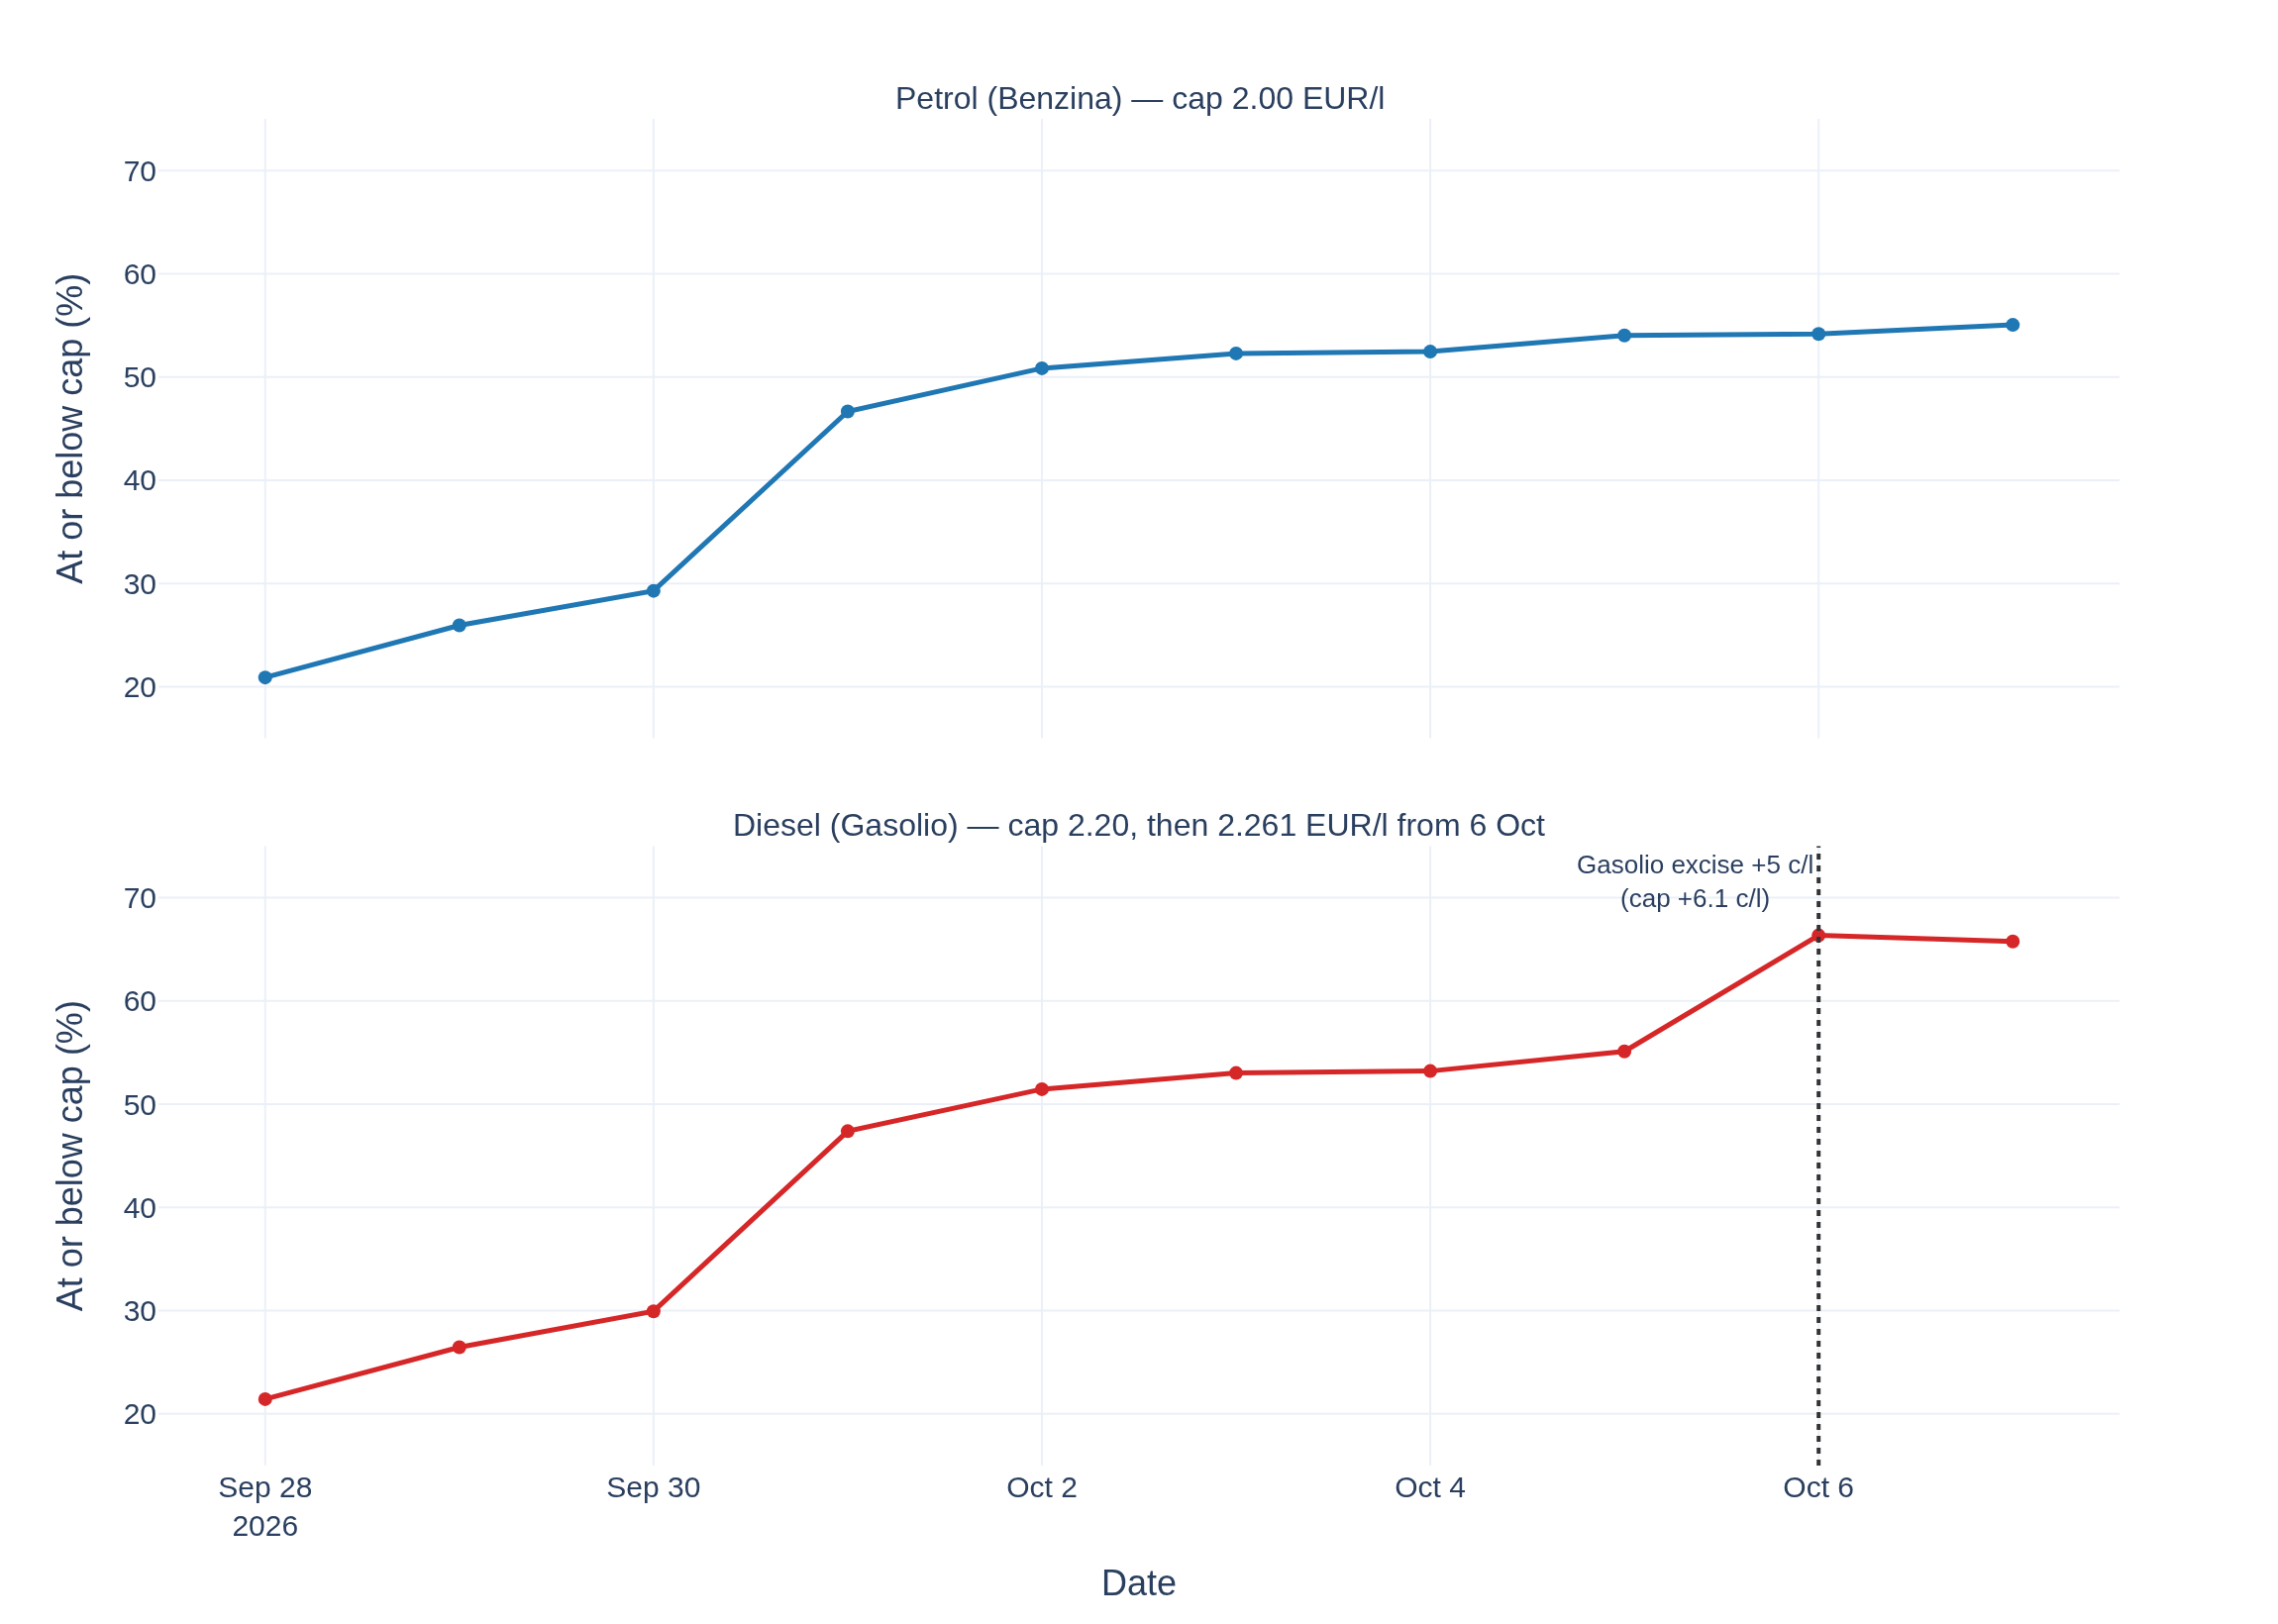
\includegraphics[width=0.92\textwidth]{output/figures/fig1_raw_adoption_share.png}
\caption{Share of stations priced at or below the cap, by day and
fuel. Exact daily shares from the dtComu-effective panel; no model, no
uncertainty bands. The dotted line in the lower (gasolio) panel marks
the excise increase of 6 October (cap threshold $+6.1$~c/l); petrol is
unaffected, so its panel has no line.}
\label{fig:rawshares}
\end{figure}

Brand gradients are stark. By 7 October, the share of station--fuel
units at or below the (fuel- and date-adjusted) cap was: Agip Eni
98.9\%, Q8 93.0\%, Tamoil 70.5\%, Api-Ip 51.0\%, Esso 51.6\%, Pompe
Bianche (independents) 35.4\%. Mean prices order identically
(\cref{fig:prices}): the market split into a cap-following tier and an
above-cap tier, with Agip Eni locking at 1.99~\euro/l from the cap day
while Q8 followed only with its 1 October wave.

\begin{figure}[htbp]
\centering
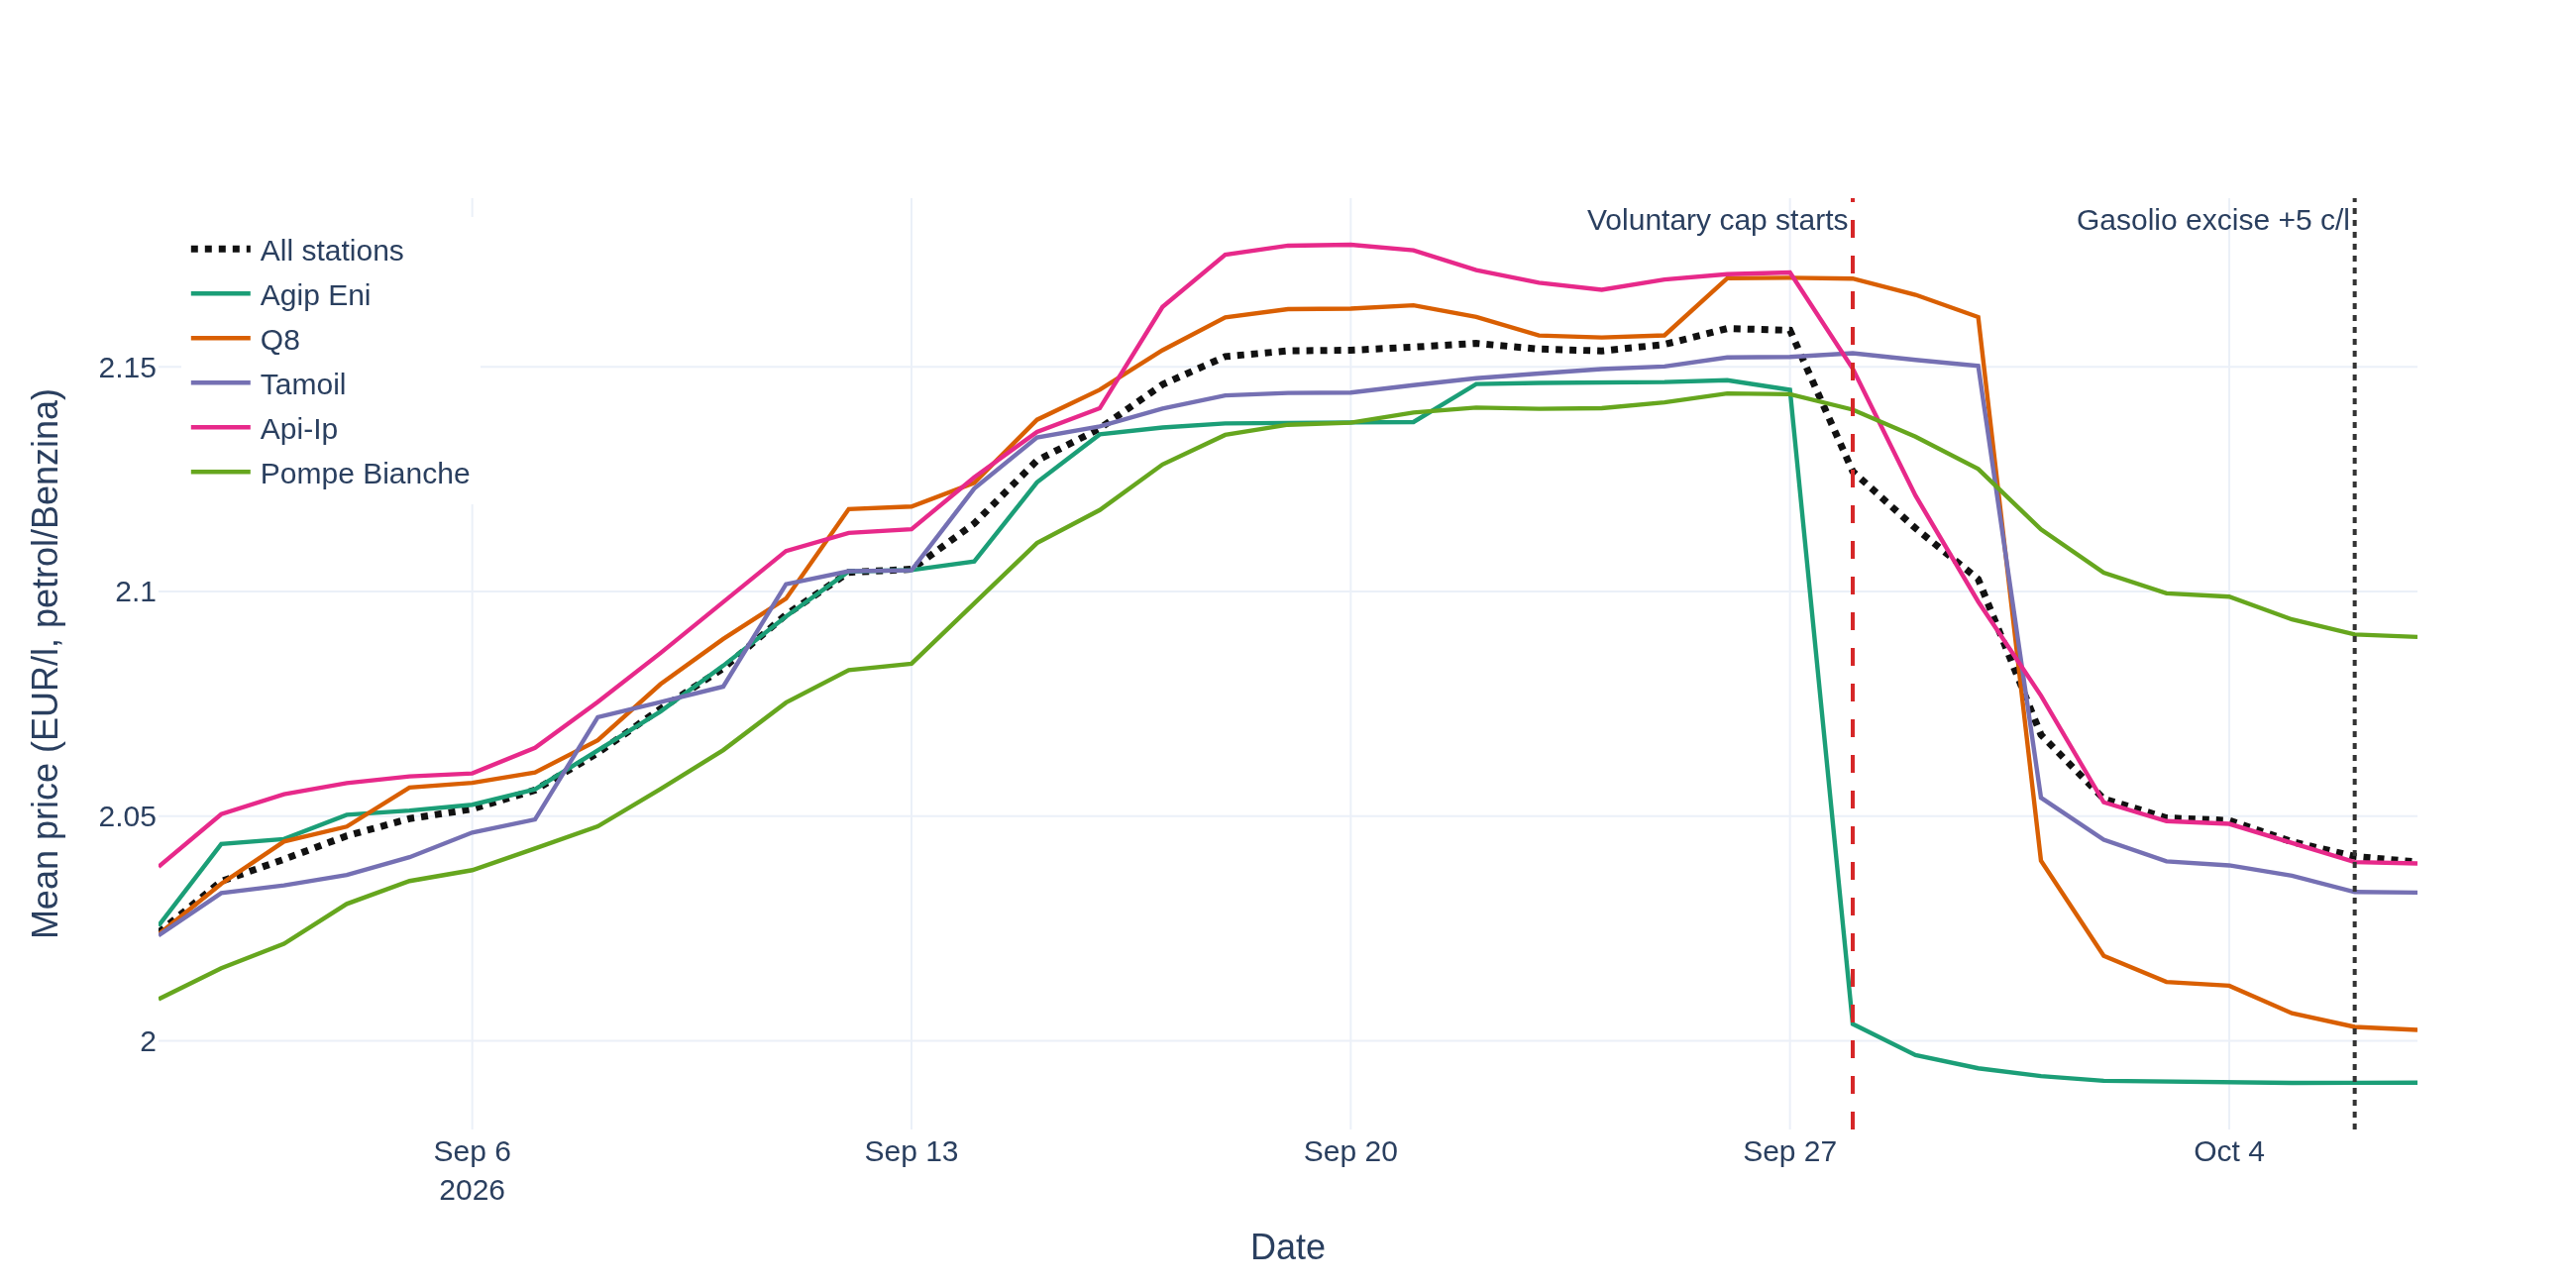
\includegraphics[width=0.92\textwidth]{output/figures/fig_prices_daily.png}
\caption{Daily mean pump price (petrol), 1 September -- 6 October 2026:
all stations (black dotted) and the five largest brands. Dashed red
line: voluntary cap starts (28 Sep); dotted line: gasolio excise
increase (6 Oct).}
\label{fig:prices}
\end{figure}

Geographically, adoption was highest around Rome and the
central-northern coastal corridors and lowest in the Po-valley fringes
and parts of the South (\cref{fig:mapall}).

\begin{figure}[H]
\centering
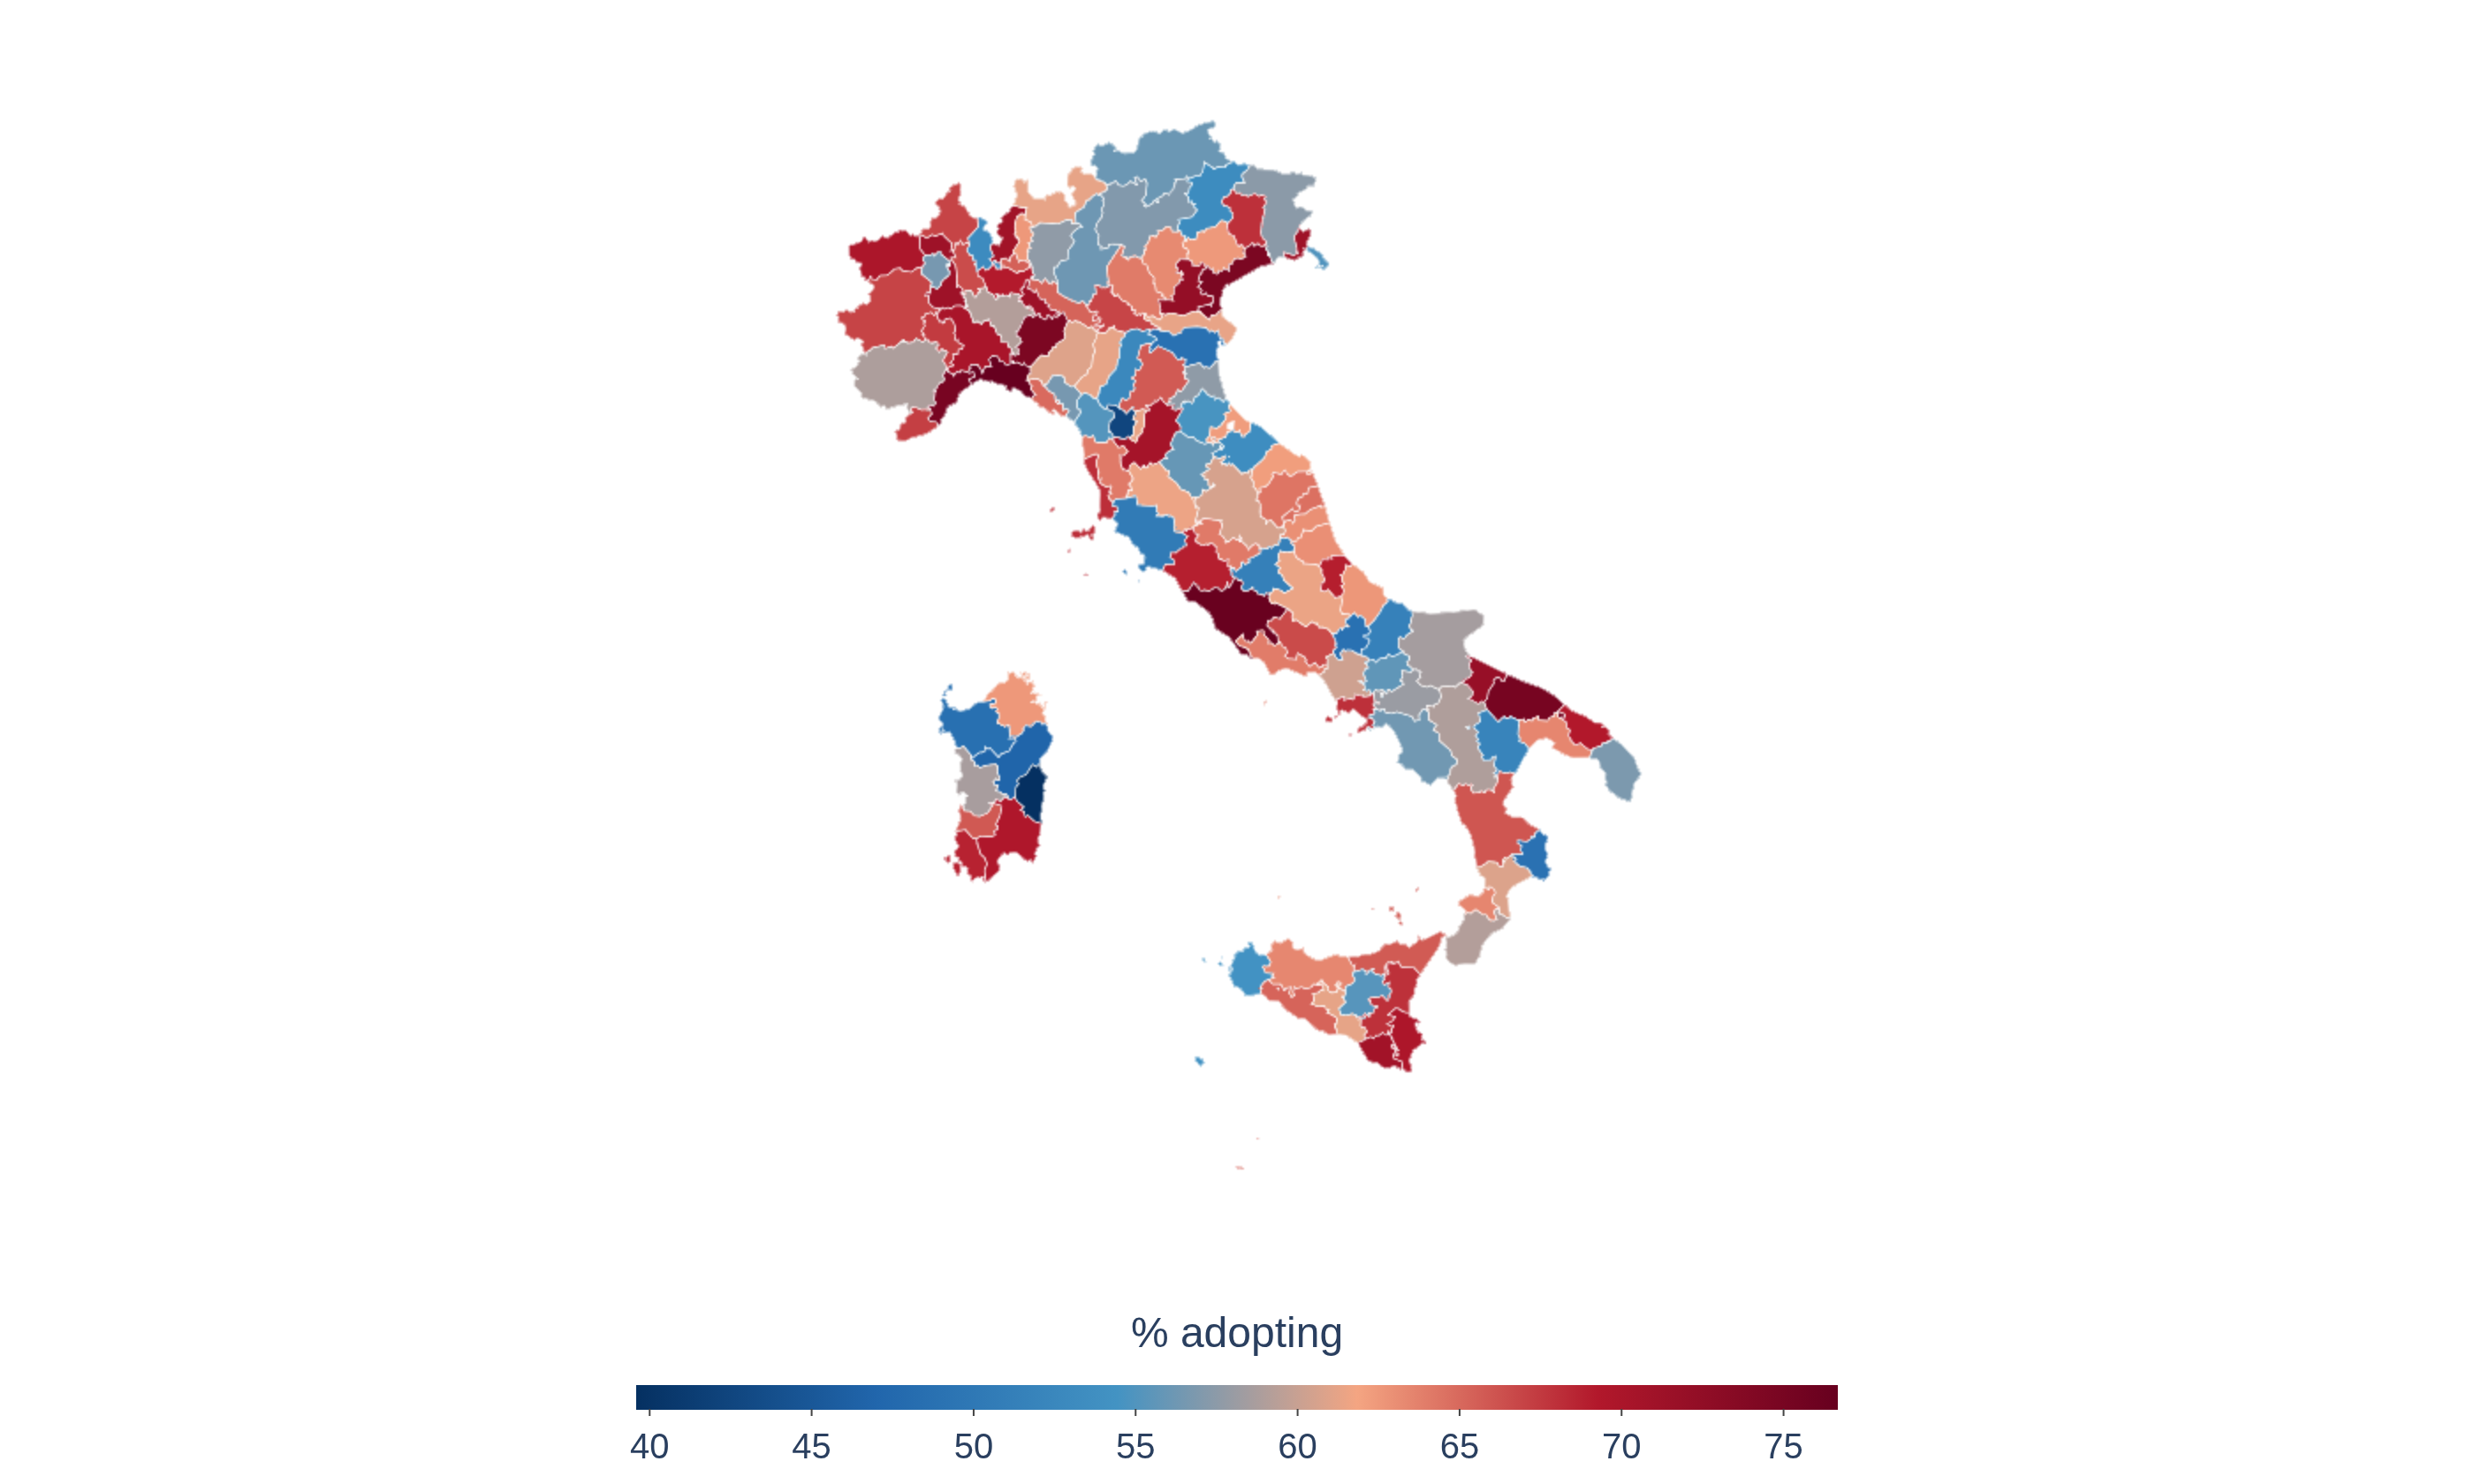
\includegraphics[width=0.8\textwidth]{output/figures/map_adoption_share.png}
\caption{Share of stations adopting the cap by province (all stations;
station--fuel units, any day 28 Sep -- 7 Oct 2026, tax-adjusted
threshold).}
\label{fig:mapall}
\end{figure}

\begin{figure}[H]
\centering
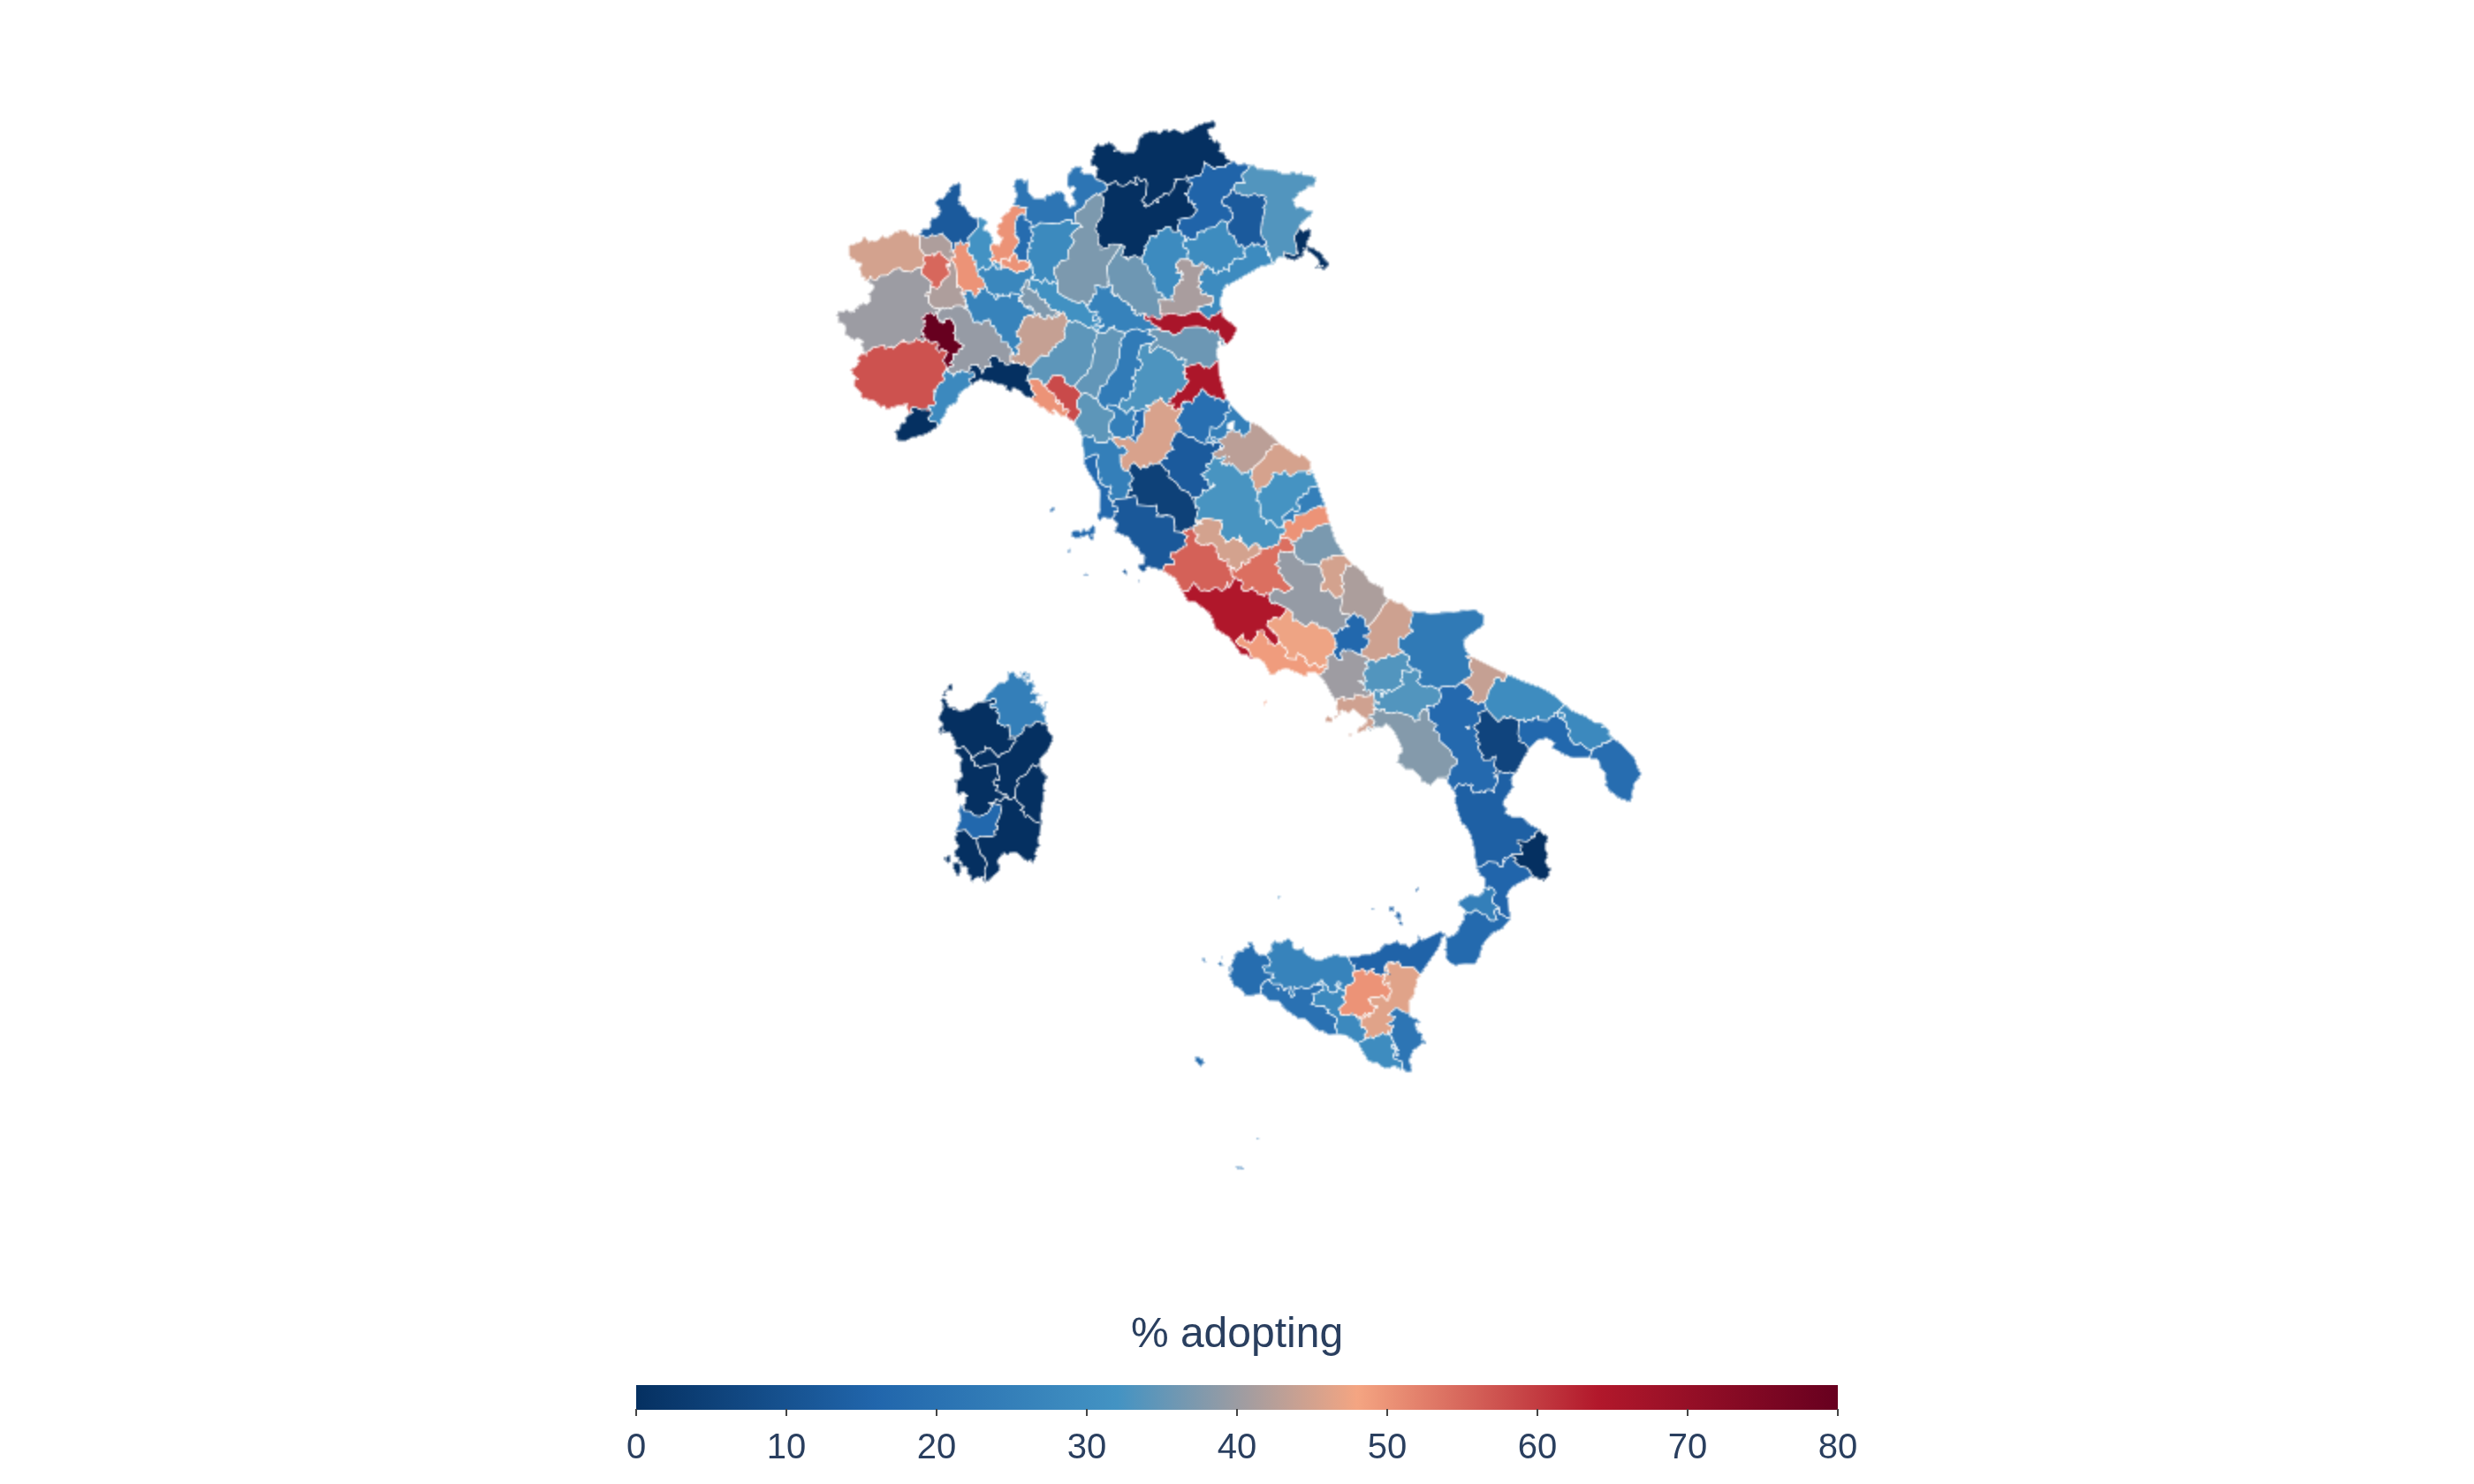
\includegraphics[width=0.8\textwidth]{output/figures/map_pb_adoption_share.png}
\caption{Share of Pompe Bianche (independent) stations adopting the cap,
by province.}
\label{fig:mappb}
\end{figure}

The overall map (\cref{fig:mapall}) shows a clear geography: adoption
was highest around Rome, along the Tyrrhenian corridor and in parts of
the North-West (up to 69\% of units), and lowest in Alpine provinces
and parts of the South and the islands (down to 31\%). The range is
wide --- a 38-percentage-point gap between the extremes --- and the
north--south gradient is not monotone: some southern provinces
(Abruzzo's corridor, coastal Puglia) match northern adoption levels.
The independents' map is strikingly different (\cref{fig:mappb}):
independent adoption rates are low almost everywhere (national mean
23\%, and exactly zero in the darkest provinces) with a sharp pocket of
convergence along the central Adriatic axis --- from Umbria through the
Marche -- Abruzzo corridor --- where independents followed the leader's
network, and near-zero adoption in the Alpine arc and the islands.
Independents responded to local pressure, not to the national
announcement.

\section{Who adopts? Survival analysis}
\label{sec:survival}

We estimate Cox proportional-hazards models \parencite{cox1972regression}
of time to adoption. Duration is days from 28 September to first at-cap
day; never-adopters are right-censored at 7 October, and the gasolio
threshold is tax-adjusted from 6 October. Because brand
differences are so stark in the raw data --- and because the leader's own
stations adopted almost mechanically by construction --- we estimate the
model on three samples: the \emph{universe} of station--fuel units; the
market \emph{excluding} Agip Eni and Q8 (the two brands that announced
at-cap prices in the first wave); and \emph{Pompe Bianche only}
(independent stations). Standard errors are clustered by Gestore
(operator). Chain size counts stations nationwide under the same Gestore.

% Auto-generated: do not edit by hand.
% Source: R/revision_samples.R -> output/revision_{cox,lpm}.txt
% Panel window: 2026-09-28 .. 2026-10-07, gasolio cap tax-adjusted (+6.1 c/l from 2026-10-06).

\begin{table}[htbp]
\centering
\caption{Cox duration-model estimates by sample (coefficients; hazard ratios $=e^{\hat\beta}$)}
\label{tab:cox-samples}
\begin{tabular}{lccc}
\toprule
 & (1) Universe & (2) Excl.\ Agip Eni + Q8 & (3) Pompe Bianche \\
\midrule
Nearest station (km) & -0.0955$^{***}$ & -0.0687$^{***}$ & -0.1424$^{***}$ \\
Nearest day-0 adopter (km) & -0.0219$^{***}$ & -0.0512$^{***}$ & -0.0597$^{***}$ \\
Population per 1-km cell & 0.0000$^{***}$ & 0.0000$^{**}$ & 0.0000 \\
Pre-cap gap (\euro/l) & -4.2130$^{***}$ & -6.5050$^{***}$ & -5.3770$^{***}$ \\
Chain size (Gestore, stations) & 0.0006$^{***}$ & 0.0008$^{***}$ & 0.0076$^{***}$ \\
Gasolio & 0.1727$^{***}$ & 0.3236$^{***}$ & 0.5716$^{***}$ \\
\midrule
N & 39,418\ & 26,709\ & 5,198\ \\
Events & 25,113\ & 12,854\ & 1,842\ \\
\bottomrule
\end{tabular}

\medskip
\footnotesize Gestore-clustered robust standard errors. All models
include a Gasolio dummy. The gasolio cap threshold is adjusted for the
excise change of 6 October 2026 (see \cref{sec:data}).
\end{table}



\Cref{tab:cox-samples} reports coefficients (hazard ratios are
$e^{\hat\beta}$). Three results are robust across samples. First, the
\textbf{pre-cap gap dominates}: its coefficient grows (in magnitude) from
$-4.2$ in the universe to $-6.5$ excluding the leader brands and
$-5.4$ for independents --- stations already pricing near the cap adopted
almost mechanically, and this remains the single strongest predictor
once leader stations are removed. Second, \textbf{spatial spillovers
strengthen when the leader brands are removed}: the nearest-adopter
distance coefficient triples from $-0.022$ (universe) to $-0.051$
(excl.\ Agip Eni/Q8) and $-0.060$ (Pompe Bianche). This is exactly the
pattern strategic-complementarity models predict: leader-brand rows
absorbed the spatial variation, and once they are excluded, the
neighbourhood diffusion effect emerges clearly. Independents respond to
what nearby stations do, not to the cap announcement itself. Third,
\textbf{chain size matters most for independents} ($0.008$ versus
$0.001$): small local chains (gestori) coordinated their response,
while brand-level headquarters decided for the organised brands.

Robustness. A Weibull AFT model gives the same signs and significance
per sample; gestore-clustered standard errors leave all conclusions
unchanged; the PH assumption is examined in \cref{app:diag} and the
reported coefficients should be read as window-averaged effects.

\section{Market dynamics: panel event study and adoption probabilities}
\label{sec:panel}

\subsection{Event study}

We estimate station fixed-effects models of the daily at-cap indicator
over the event window $[-7, +7]$ around the cap:
\begin{equation}
\text{at\_cap}_{it} = \sum_{k \ne -1} \beta_k \,
\mathbf{1}[t - T_0 = k] + \alpha_i + \varepsilon_{it},
\label{eq:es}
\end{equation}
with day $-1$ as reference and gestore-clustered errors. Because
\cref{fig:rawshares} already shows the raw adoption path --- the data are
exhaustive, so the shares themselves carry no sampling uncertainty ---
the event study serves only as a robustness check that the pattern is
not an artefact of composition. Its coefficients are reported in
\cref{app:es} and mirror \cref{fig:rawshares}: no pre-cap movement, a
jump at day 0, and a plateau from day 5.

To trace diffusion, we split station--fuel units into terciles by their
distance to the nearest station that adopted on day 0 (cut points:
1.08 and 3.15~km) and plot the exact daily at-cap share of each tercile
in \cref{fig:capdist}. The three curves never cross. At every point in
time, stations near a day-0 adopter adopt earlier and more often: on
5 October, 62.7\% of the near tercile is at the cap versus 44.3\% of
the far tercile --- an 18-percentage-point gradient --- and the far
tercile never catches up over our window. Note that the far tercile's
curve is not flat either: it rises throughout, so diffusion eventually
reached remote stations too, but with a lag of several days. This
ordering is exactly what local strategic complementarities predict, and
it is invisible in the aggregate series of \cref{fig:rawshares}.

\begin{figure}[htbp]
\centering
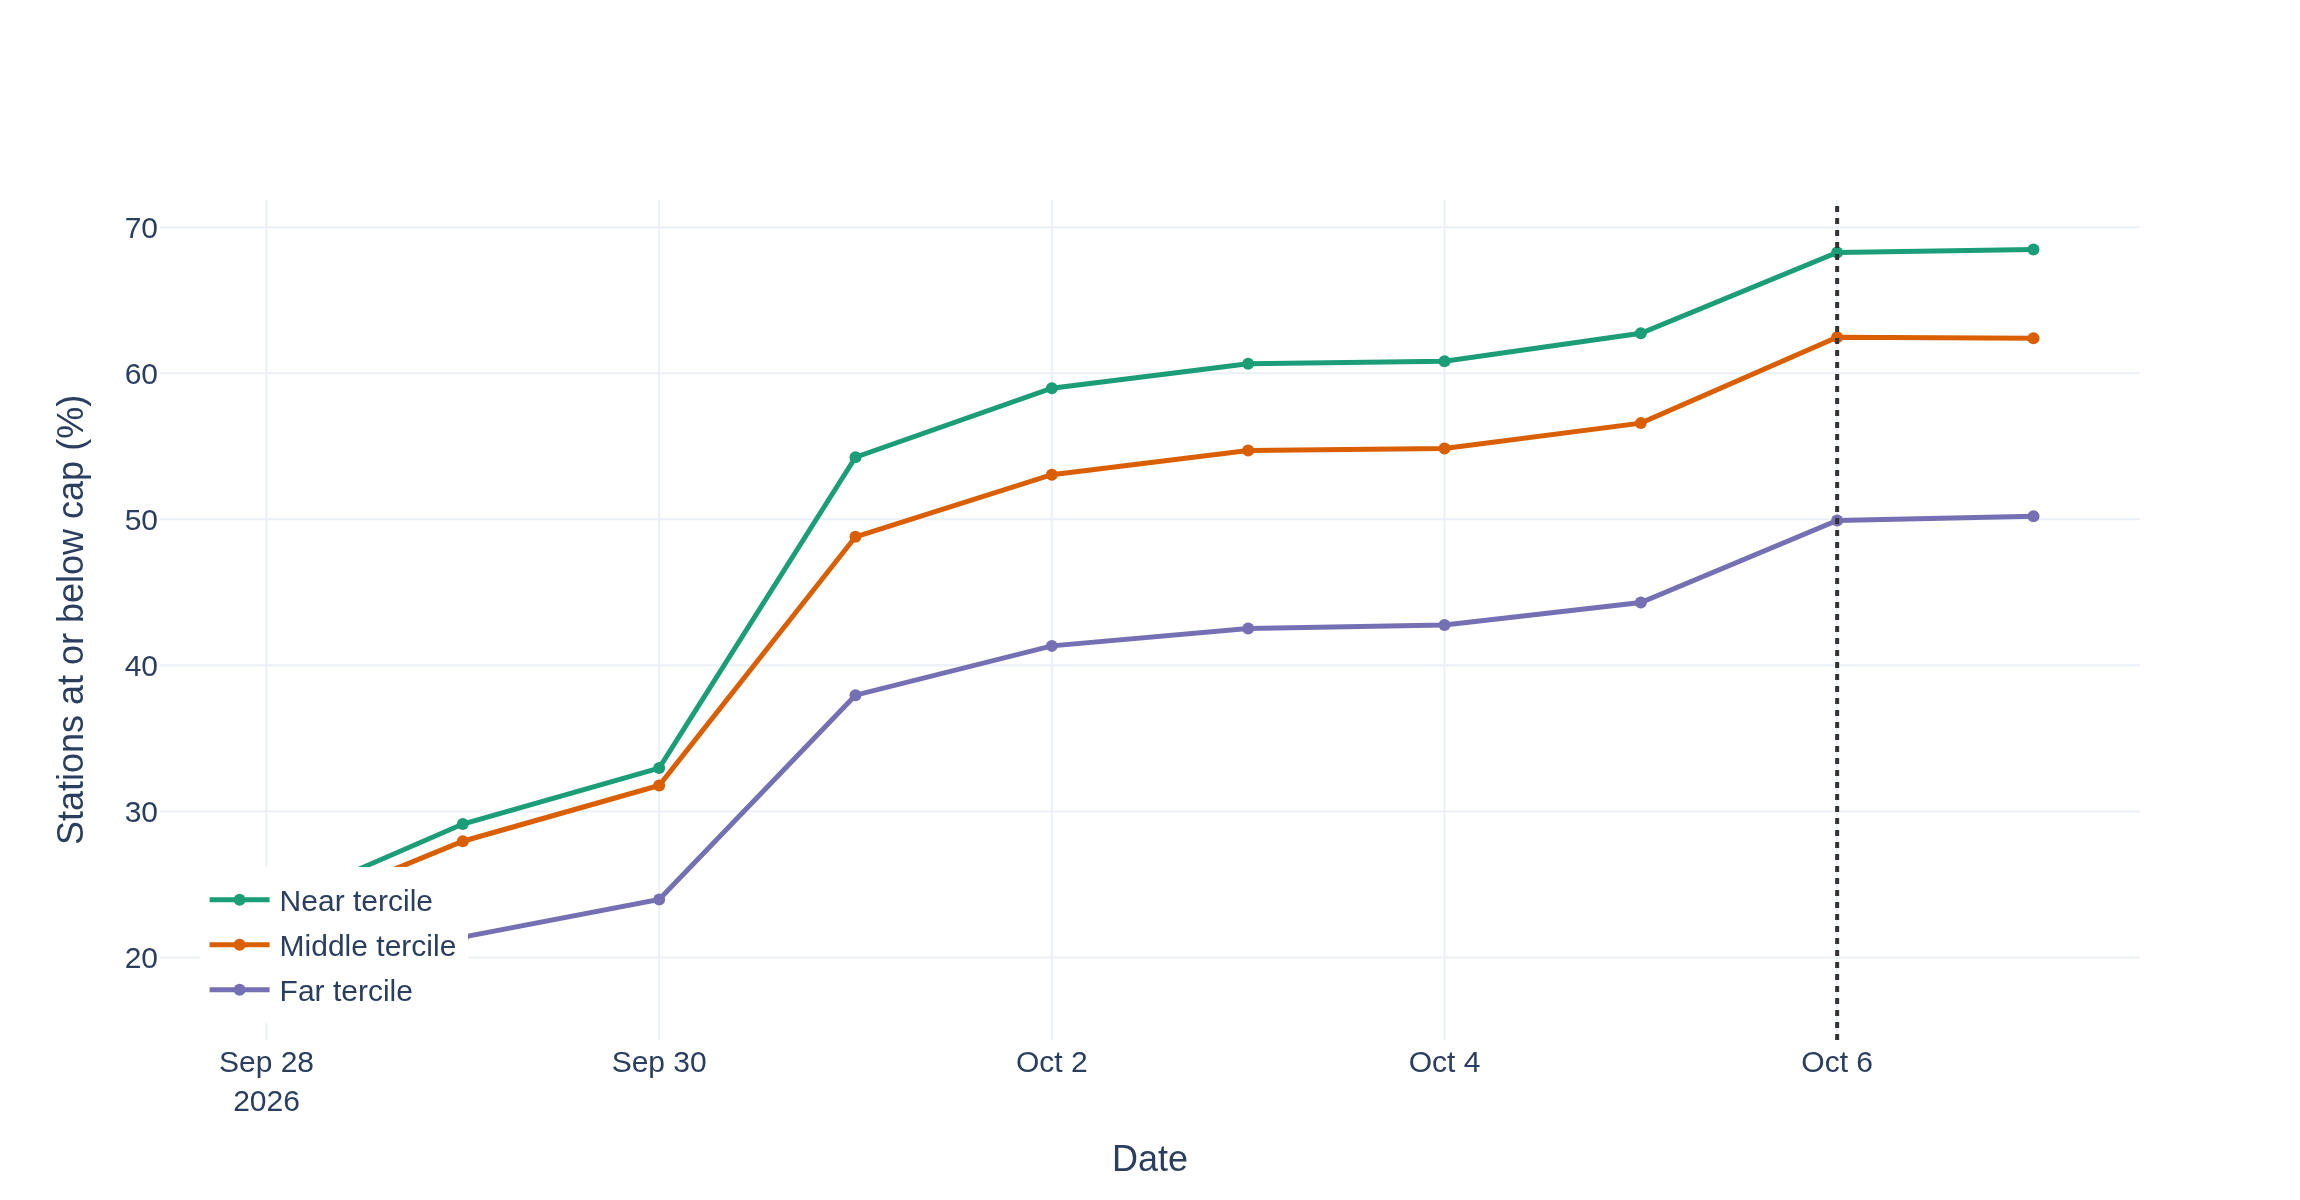
\includegraphics[width=0.85\textwidth]{output/figures/event_study_by_capdist.png}
\caption{Stations at or below the cap by distance to the nearest day-0
adopter (terciles; exact daily shares). Cut points: 1.08 and 3.15~km.}
\label{fig:capdist}
\end{figure}

\subsection{Who adopts? Adoption probabilities}
\label{sec:lpm}

The survival analysis of \cref{sec:survival} conditions on time;
here we ask the complementary question: given the full covariate set of
\cref{sec:variables}, \emph{which} stations ended up adopting at all?
We estimate linear probability models (OLS with gestore-clustered
standard errors)
\begin{equation}
\text{adopted}_i = \mathbf{x}_i'\gamma + \mu_{b(i)} + \delta_{r(i)}
+ u_i,
\label{eq:lpm}
\end{equation}
where $\mathbf{x}_i$ collects the continuous and fuel covariates,
$\mu_b$ are brand fixed effects (within-sample \(\ge\)100-observation
rule) and $\delta_r$ region fixed effects. \Cref{tab:lpm-core} reports
the core coefficients for the same three samples as
\cref{tab:cox-samples}; the full brand and region coefficients appear in
\cref{app:lpm-s1,app:lpm-s2}.

% Auto-generated: do not edit by hand.
% Source: R/revision_samples.R -> output/revision_{cox,lpm}.txt
% Panel window: 2026-09-28 .. 2026-10-07, gasolio cap tax-adjusted (+6.1 c/l from 2026-10-06).

\begin{table}[htbp]
\centering
\caption{Adoption probability (LPM) by sample --- core covariates}
\label{tab:lpm-core}
\begin{tabular}{lccc}
\toprule
 & (1) Universe & (2) Excl.\ Agip Eni + Q8 & (3) Pompe Bianche \\
\midrule
Intercept & 1.0750$^{***}$ & 0.3511$^{**}$ & 0.4029$^{***}$ \\
Nearest station (km) & -0.0122$^{***}$ & -0.0113$^{***}$ & -0.0164$^{*}$ \\
Nearest day-0 adopter (km) & -0.0100$^{***}$ & -0.0137$^{***}$ & -0.0100$^{***}$ \\
Population per 1-km cell & 0.0000 & 0.0000$^{*}$ & 0.0000 \\
Pre-cap gap (\euro/l) & -1.2837$^{***}$ & -1.6059$^{***}$ & -1.0700$^{***}$ \\
Chain size (Gestore, stations) & 0.0001$^{***}$ & 0.0000 & 0.0019$^{***}$ \\
Gasolio & 0.1051$^{***}$ & 0.1477$^{***}$ & 0.1950$^{***}$ \\
Brand \& region FE & Yes & Yes & Region only \\
\midrule
N & 39338 & 26662 & 5180 \\
Adj.~$R^2$ & 0.3560 & 0.2038 & 0.2476 \\
\bottomrule
\end{tabular}

\medskip
\footnotesize Dependent variable: adopted (=1 if the station--fuel unit
priced at or below the cap on any day 28 Sep -- 7 Oct 2026; the gasolio
cap is tax-adjusted from 6 Oct). OLS with gestore-clustered standard
errors. Brand reference: Agip Eni in columns (1), Ala in column (2);
region reference: Abruzzo. Full brand and region coefficients in
\cref{app:lpm-s1,app:lpm-s2}. In column (3) the sample is single-brand
(Pompe Bianche), so brand FE are undefined.
\end{table}



The LPM confirms and sharpens the survival results. The pre-cap gap is
by far the strongest predictor in every sample: $-1.28$ probability
points per cent/litre of pre-cap excess in the universe sample, $-1.61$
excluding the leader brands, $-1.07$ for independents. Distance to the
nearest day-0 adopter is negative and significant in all three samples
($-0.010$ universe, $-0.014$ excluding the leader brands, $-0.010$ for
Pompe Bianche), while the distance to the nearest station
(competitor) is smaller and only marginally significant for
independents ($-0.016$, $p = 0.014$): proximity to \emph{adopters}
predicts adoption at least as strongly as proximity to competitors,
and for independents the two effects are of similar magnitude once
measurement noise is accounted for. Chain size is positive and
significant in the universe and Pompe Bianche samples (insignificant
once the leader brands are removed, whose networks coordinate centrally)
and roughly nineteen times larger for Pompe Bianche, echoing the
gestore-coordination reading of \cref{sec:survival}. Population density
is economically negligible once brand and region are controlled. Fit is
moderate (adjusted $R^2 = 0.20$--$0.36$), as expected for individual
adoption decisions; diagnostics are in \cref{app:diag}.

\section{Dispersion and competitiveness}
\label{sec:dispersion}

\paragraph{Province-level dispersion.}
We compute, for each province $\times$ fuel $\times$ phase (pre:
21--27 September; post: 28 September -- 7 October), the daily
within-province standard deviation of effective prices, and compare
phases. The SD rose in \textbf{217 of the 220 province--fuel cells}
(98.6\%): on average from 50 to 92~c/l for petrol and from 65 to
102~c/l for diesel --- a doubling. \Cref{fig:sdpre,fig:sdpost} show the
distribution of the shift. Throughout the paper, maps use a blue--red
scale: \emph{blue marks low values and red marks high values}. The
province-level standard deviation rises from a median of 50~c/l
pre-cap to 90~c/l post-cap, and the whole distribution shifts right
(\cref{fig:sdcapdist}, top panel): 217 of the 220 province--fuel cells
see their SD increase. \Cref{fig:sdpre,fig:sdpost} in \cref{app:maps}
show the geography: pre-cap the map is predominantly light blue
(typical SDs 28--150~c/l); post-cap red spreads along the Alps and the
Apennines --- the provinces where dispersion widened most are those
where the adopter share was intermediate, mixing cap-priced with
above-cap stations. Provincial SDs after the cap run 71--235~c/l, and
no province returns to its pre-cap level. The cap did not compress the
distribution --- it split it. A mass of adopters sits exactly at the
threshold while a non-adopter tail holds prices above it, producing a
bimodal distribution unlike the smooth equilibrium-dispersion
benchmarks \parencite{reinganum1979, stiglitz1982}.

\begin{figure}[H]
\centering
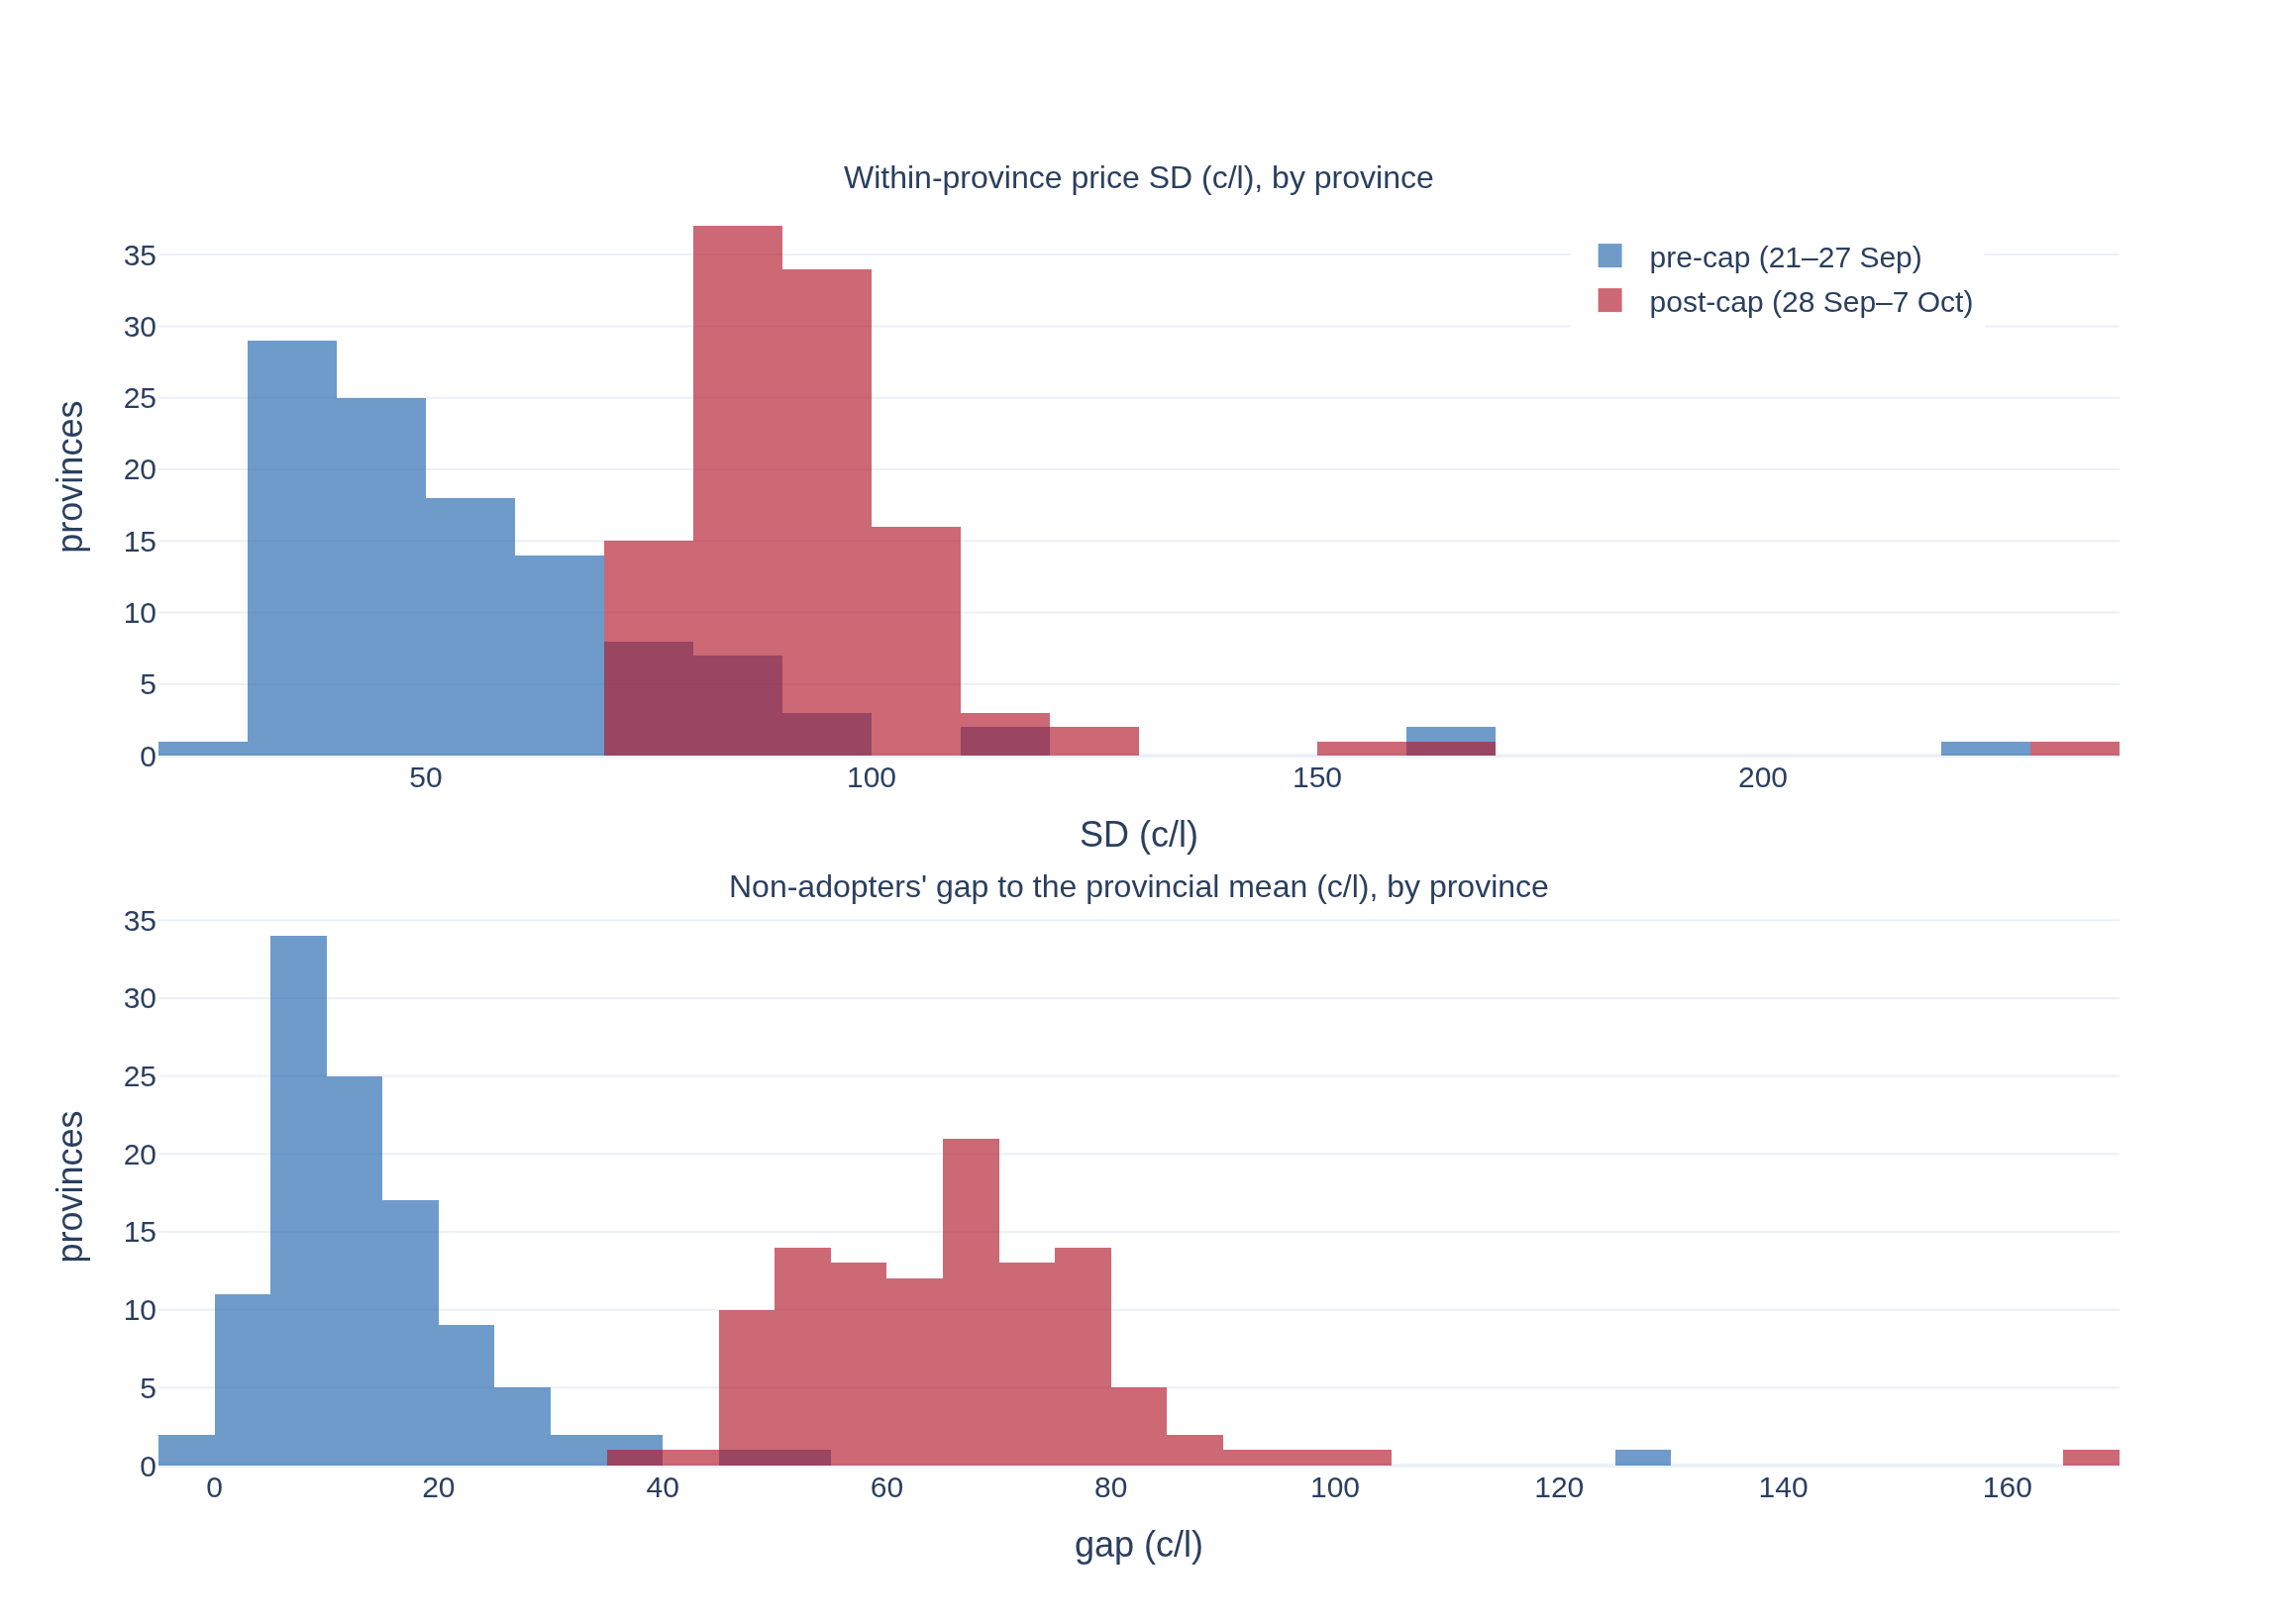
\includegraphics[width=0.85\textwidth]{output/figures/fig_dispersion_hist.png}
\caption{Province-level distributions before (blue) and after (red) the
cap. Top: within-province standard deviation of effective prices.
Bottom: non-adopters' mean gap to the provincial daily mean.}
\label{fig:sdcapdist}
\end{figure}

The consumer reading is correspondingly uneven: where adoption was high,
prices fell to the cap for most of the market; where the non-adopter
tail dominated, prices barely moved. Given that adoption tracked
population density and chain presence, the gains concentrate in urban,
organised-firm corridors --- with distributional implications for
car-dependent rural areas \parencite{mattioli2023}.

\section{Conclusions}
\label{sec:conclusion}

A voluntary, temporary price cap announced by the Italian market leader
achieved partial market-wide matching within days --- by 7 October 58\%
of petrol and 69\% of gasolio station--fuel units priced at or below
the (tax-adjusted) threshold. Adoption was primarily a firm decision --- but not only: once the
leader brands are excluded, local spillovers emerge as a first-order
driver, with the adoption hazard falling 7--14\% per kilometre from the
nearest adopter and independent stations following in dense, organised
corridors while ignoring the cap elsewhere. Pre-cap price position
dominates everywhere: stations already pricing near the threshold
adopted almost mechanically. The cap polarised rather than compressed
the market: dispersion widened in almost every province, and
non-adopters became relatively more expensive. Consumer gains are
therefore real but geographically uneven --- visible in the north-south
and brand gradients of the adoption maps.

Three caveats. First, our window is nine post-cap days; the two-month
cap horizon may produce further convergence or reversal around expiry
--- strategic pricing near sunset dates is unobservable here. Second,
adoption is measured from communications; enforcement (actual pump
prices versus communicated ones) is outside our data. Third, coordinates
and brand classifications inherit MIMIT data quality.

For measurement, our snapshot-bias result is a caution for official
statistics: reference-day sampling from 8am-cut extracts mis-dated an
entire communication wave in October 2026, overstating reference-day
averages by 3.5--4.1~c/l. Communication-time reconstruction, as
implemented here, is the robust alternative.

\printbibliography

\appendix

\section*{Appendix}
\addcontentsline{toc}{section}{Appendix}

\renewcommand{\thesection}{\Alph{section}}
\setcounter{section}{0}

\section{Event-study coefficients}
\label{app:es}

\begin{table}[htbp]
\centering
\caption{Station-FE event-study coefficients (\cref{eq:es})}
\label{tab:es-coefs}
\begin{tabular}{lcc}
\toprule
Event time & $\hat\beta_k$ & Std.~error \\
\midrule
Day +0 & 0.193$^{***}$ & 0.037 \\
Day +1 & 0.243$^{***}$ & 0.037 \\
Day +2 & 0.277$^{***}$ & 0.037 \\
Day +3 & 0.451 & 0.046 \\
Day +4 & 0.492 & 0.044 \\
Day +5 & 0.507 & 0.042 \\
Day +6 & 0.509 & 0.042 \\
Day +7 & 0.526 & 0.040 \\
\bottomrule
\end{tabular}

\medskip
\footnotesize Dependent variable: at-cap indicator; station fixed
effects; gestore-clustered errors; day $-1$ = 27 September omitted.
Pre-cap coefficients are small and insignificant; the jump occurs at
$k=0$ and the series plateaus from $k=5$.
\end{table}


\section{Full LPM coefficient tables}
\label{app:lpm-full}

Brand and region fixed-effect estimates for the linear probability
models of \cref{sec:lpm} are reported in \cref{app:lpm-s1,app:lpm-s2}.

% Auto-generated: do not edit by hand.
% Source: R/revision_samples.R -> output/revision_{cox,lpm}.txt
% Panel window: 2026-09-28 .. 2026-10-07, gasolio cap tax-adjusted (+6.1 c/l from 2026-10-06).

\begin{table}[htbp]
\centering
\caption{Adoption probability (LPM), universe sample --- brand and region fixed effects}
\label{app:lpm-s1}
\begin{tabular}{lr}
\toprule
 & Coefficient \\
\midrule
Brand: Ala & -0.7860$^{***}$ \\
Brand: Api-Ip & -0.4597$^{***}$ \\
Brand: Aquila & -0.8722$^{***}$ \\
Brand: Beyfin & -0.6594$^{***}$ \\
Brand: COIL & -0.2664$^{***}$ \\
Brand: CONAD & -0.0949$^{**}$ \\
Brand: Costantin & -0.1879$^{**}$ \\
Brand: Ego & -0.6950$^{***}$ \\
Brand: Energas & -0.1541 \\
Brand: Enerpetroli & -0.5358$^{***}$ \\
Brand: Esso & -0.4486$^{***}$ \\
Brand: Europam & -0.2427 \\
Brand: Giap & -0.2989$^{***}$ \\
Brand: Itala Petroli & -0.5340$^{***}$ \\
Brand: KEROPETROL & -0.8392$^{***}$ \\
Brand: Loro & -0.8784$^{***}$ \\
Brand: Lukoil & -0.5499$^{***}$ \\
Brand: OTHER & -0.5202$^{***}$ \\
Brand: Petrol Gamma & -0.6479$^{***}$ \\
Brand: Pompe Bianche & -0.6412$^{***}$ \\
Brand: Q8 & -0.0870$^{***}$ \\
Brand: Retitalia & -0.7426$^{***}$ \\
Brand: San Marco Petroli & -0.9128$^{***}$ \\
Brand: Shell & -0.7493$^{***}$ \\
Brand: Sia fuel & -0.3296$^{***}$ \\
Brand: Tamoil & -0.2704$^{***}$ \\
Brand: Toil & -0.5352$^{***}$ \\
Brand: Vega & -0.2015$^{***}$ \\
Region: Abruzzo & 0.1104 \\
Region: Basilicata & 0.1189 \\
Region: Calabria & 0.0900 \\
Region: Campania & 0.1240 \\
Region: Emilia-Romagna & 0.0431 \\
Region: Friuli-Venezia Giulia & 0.0283 \\
Region: Lazio & 0.1342 \\
Region: Liguria & 0.1041 \\
Region: Lombardia & 0.0464 \\
Region: Marche & 0.0700 \\
Region: Molise & 0.0134 \\
Region: Piemonte & 0.0627 \\
Region: Puglia & 0.1043 \\
Region: Sardegna & 0.0307 \\
Region: Sicilia & 0.0904 \\
Region: Toscana & 0.0562 \\
Region: Umbria & 0.1012 \\
Region: Veneto & 0.0936 \\
Brand: Api-Ip & 0.3133$^{***}$ \\
Brand: Aquila & -0.0879 \\
Brand: Beyfin & 0.1238 \\
Brand: COIL & 0.5018$^{***}$ \\
Brand: CONAD & 0.6668$^{***}$ \\
Brand: Costantin & 0.5927$^{***}$ \\
Brand: Ego & 0.0815 \\
Brand: Energas & 0.5948$^{***}$ \\
Brand: Enerpetroli & 0.2185$^{***}$ \\
Brand: Esso & 0.3270$^{***}$ \\
Brand: Europam & 0.5300$^{**}$ \\
Brand: Giap & 0.5098$^{***}$ \\
Brand: Itala Petroli & 0.2315$^{***}$ \\
Brand: KEROPETROL & -0.0527 \\
Brand: Loro & -0.1056$^{***}$ \\
Brand: Lukoil & 0.2230$^{**}$ \\
Brand: OTHER & 0.2513$^{***}$ \\
\bottomrule
\end{tabular}

\medskip
\footnotesize Continuation of \cref{tab:lpm-core} column (1). Brand
reference: Agip Eni; region reference: Abruzzo. Brands with fewer
than 100 observations are grouped into OTHER.
\end{table}

% Auto-generated: do not edit by hand.
% Source: R/revision_samples.R -> output/revision_{cox,lpm}.txt
% Panel window: 2026-09-28 .. 2026-10-07, gasolio cap tax-adjusted (+6.1 c/l from 2026-10-06).

\begin{table}[htbp]
\centering
\caption{Adoption probability (LPM), excluding Agip Eni and Q8 --- brand and region fixed effects}
\label{app:lpm-s2}
\begin{tabular}{lr}
\toprule
 & Coefficient \\
\midrule
Brand: Api-Ip & 0.3133$^{***}$ \\
Brand: Aquila & -0.0879 \\
Brand: Beyfin & 0.1238 \\
Brand: COIL & 0.5018$^{***}$ \\
Brand: CONAD & 0.6668$^{***}$ \\
Brand: Costantin & 0.5927$^{***}$ \\
Brand: Ego & 0.0815 \\
Brand: Energas & 0.5948$^{***}$ \\
Brand: Enerpetroli & 0.2185$^{***}$ \\
Brand: Esso & 0.3270$^{***}$ \\
Brand: Europam & 0.5300$^{**}$ \\
Brand: Giap & 0.5098$^{***}$ \\
Brand: Itala Petroli & 0.2315$^{***}$ \\
Brand: KEROPETROL & -0.0527 \\
Brand: Loro & -0.1056$^{***}$ \\
Brand: Lukoil & 0.2230$^{**}$ \\
Brand: OTHER & 0.2513$^{***}$ \\
Brand: Petrol Gamma & 0.1071$^{*}$ \\
Brand: Pompe Bianche & 0.1179$^{***}$ \\
Brand: Retitalia & 0.0408 \\
Brand: San Marco Petroli & -0.1142$^{***}$ \\
Brand: Shell & 0.0290 \\
Brand: Sia fuel & 0.4586$^{***}$ \\
Brand: Tamoil & 0.5108$^{***}$ \\
Brand: Toil & 0.2156 \\
Brand: Vega & 0.5751$^{***}$ \\
Region: Abruzzo & 0.1207 \\
Region: Basilicata & 0.1189 \\
Region: Calabria & 0.1025 \\
Region: Campania & 0.1382 \\
Region: Emilia-Romagna & 0.0252 \\
Region: Friuli-Venezia Giulia & -0.0263 \\
Region: Lazio & 0.1471 \\
Region: Liguria & 0.1099 \\
Region: Lombardia & 0.0247 \\
Region: Marche & 0.0621 \\
Region: Molise & -0.0182 \\
Region: Piemonte & 0.0418 \\
Region: Puglia & 0.1188 \\
Region: Sardegna & -0.0230 \\
Region: Sicilia & 0.0651 \\
Region: Toscana & 0.0297 \\
Region: Umbria & 0.1075 \\
Region: Veneto & 0.0852 \\
Region: Abruzzo & 0.1250 \\
Region: Basilicata & -0.1070 \\
Region: Calabria & -0.0777 \\
Region: Campania & 0.0893 \\
Region: Emilia-Romagna & 0.0288 \\
Region: Friuli-Venezia Giulia & -0.0864 \\
Region: Lazio & 0.1267 \\
Region: Liguria & 0.0621 \\
Region: Lombardia & -0.0160 \\
Region: Marche & 0.0416 \\
Region: Molise & 0.0372 \\
Region: Piemonte & 0.1353 \\
Region: Puglia & -0.0386 \\
Region: Sardegna & -0.1121 \\
Region: Sicilia & 0.0184 \\
Region: Toscana & -0.0388 \\
Region: Umbria & 0.0231 \\
Region: Veneto & -0.0041 \\
\bottomrule
\end{tabular}

\medskip
\footnotesize Continues \cref{tab:lpm-core} column (2). Brand
reference: Ala; region reference: Abruzzo. Brands with fewer than
100 observations are grouped into OTHER.
\end{table}



\section{Model diagnostics}
\label{app:diag}

This appendix reports diagnostics for the Cox models of
\cref{tab:cox-samples} and the LPMs of \cref{tab:lpm-core}.

\paragraph{Collinearity.} The continuous covariates are close to
orthogonal: all pairwise correlations are below 0.62, the largest VIF is
1.6 (nearest-station distance), and the condition number of the
covariate correlation matrix is 4.5--5.7 across samples --- far below
conventional concern thresholds (VIF $> 10$, condition number $> 30$).
Pre-cap gap and the distance measures thus carry independent variation;
coefficients are not fragile to the inclusion of the others.

\paragraph{Proportional hazards (Cox).} Scaled Schoenfeld-residual
tests (\texttt{cox.zph}, KM transform) reject global PH in all samples,
driven by \emph{chain size} and, in the universe sample, the
\emph{pre-cap gap} (their coefficients attenuate as weaker,
further-from-cap stations adopt over the window). The qualitative
ranking of covariates is unaffected; the reported coefficients should
be read as window-averaged effects.

\paragraph{Functional form (Cox).} Martingale-residual correlations
with each continuous covariate are $\le |0.08|$ in all samples ---
no evidence of misspecified linearity for the distance, density and
gap variables at this scale.

\paragraph{LPM specification.} Pearson residuals have mean zero by
construction and are calibrated in the aggregate (mean predicted
adoption equals the observed share to four decimals in every sample).
The Ramsey RESET rejects exact linearity in the universe and
excl.-Agip/Q8 samples ($p < 0.001$), which is expected: the true
response surface is a probability bounded in $[0,1]$, and the LPM is
used for its readable coefficients, not for out-of-range extrapolation.
Heteroskedasticity inherent to binary outcomes is handled by the
gestore-clustered (Huber--White) standard errors reported throughout.

\clearpage
\section{Provincial maps by fuel}
\label{app:maps}

This appendix collects the province maps behind
\cref{sec:dispersion}. All maps use the same blue--red scale as the
main text: \emph{blue = low values, red = high values}.

\paragraph{Average provincial price the day before the cap (27
September).} Both fuels show the pre-cap north-west--south-east price
gradient, petrol around 2.00--2.20~\euro/l and diesel around
2.20--2.40~\euro/l.

\begin{figure}[H]
\centering
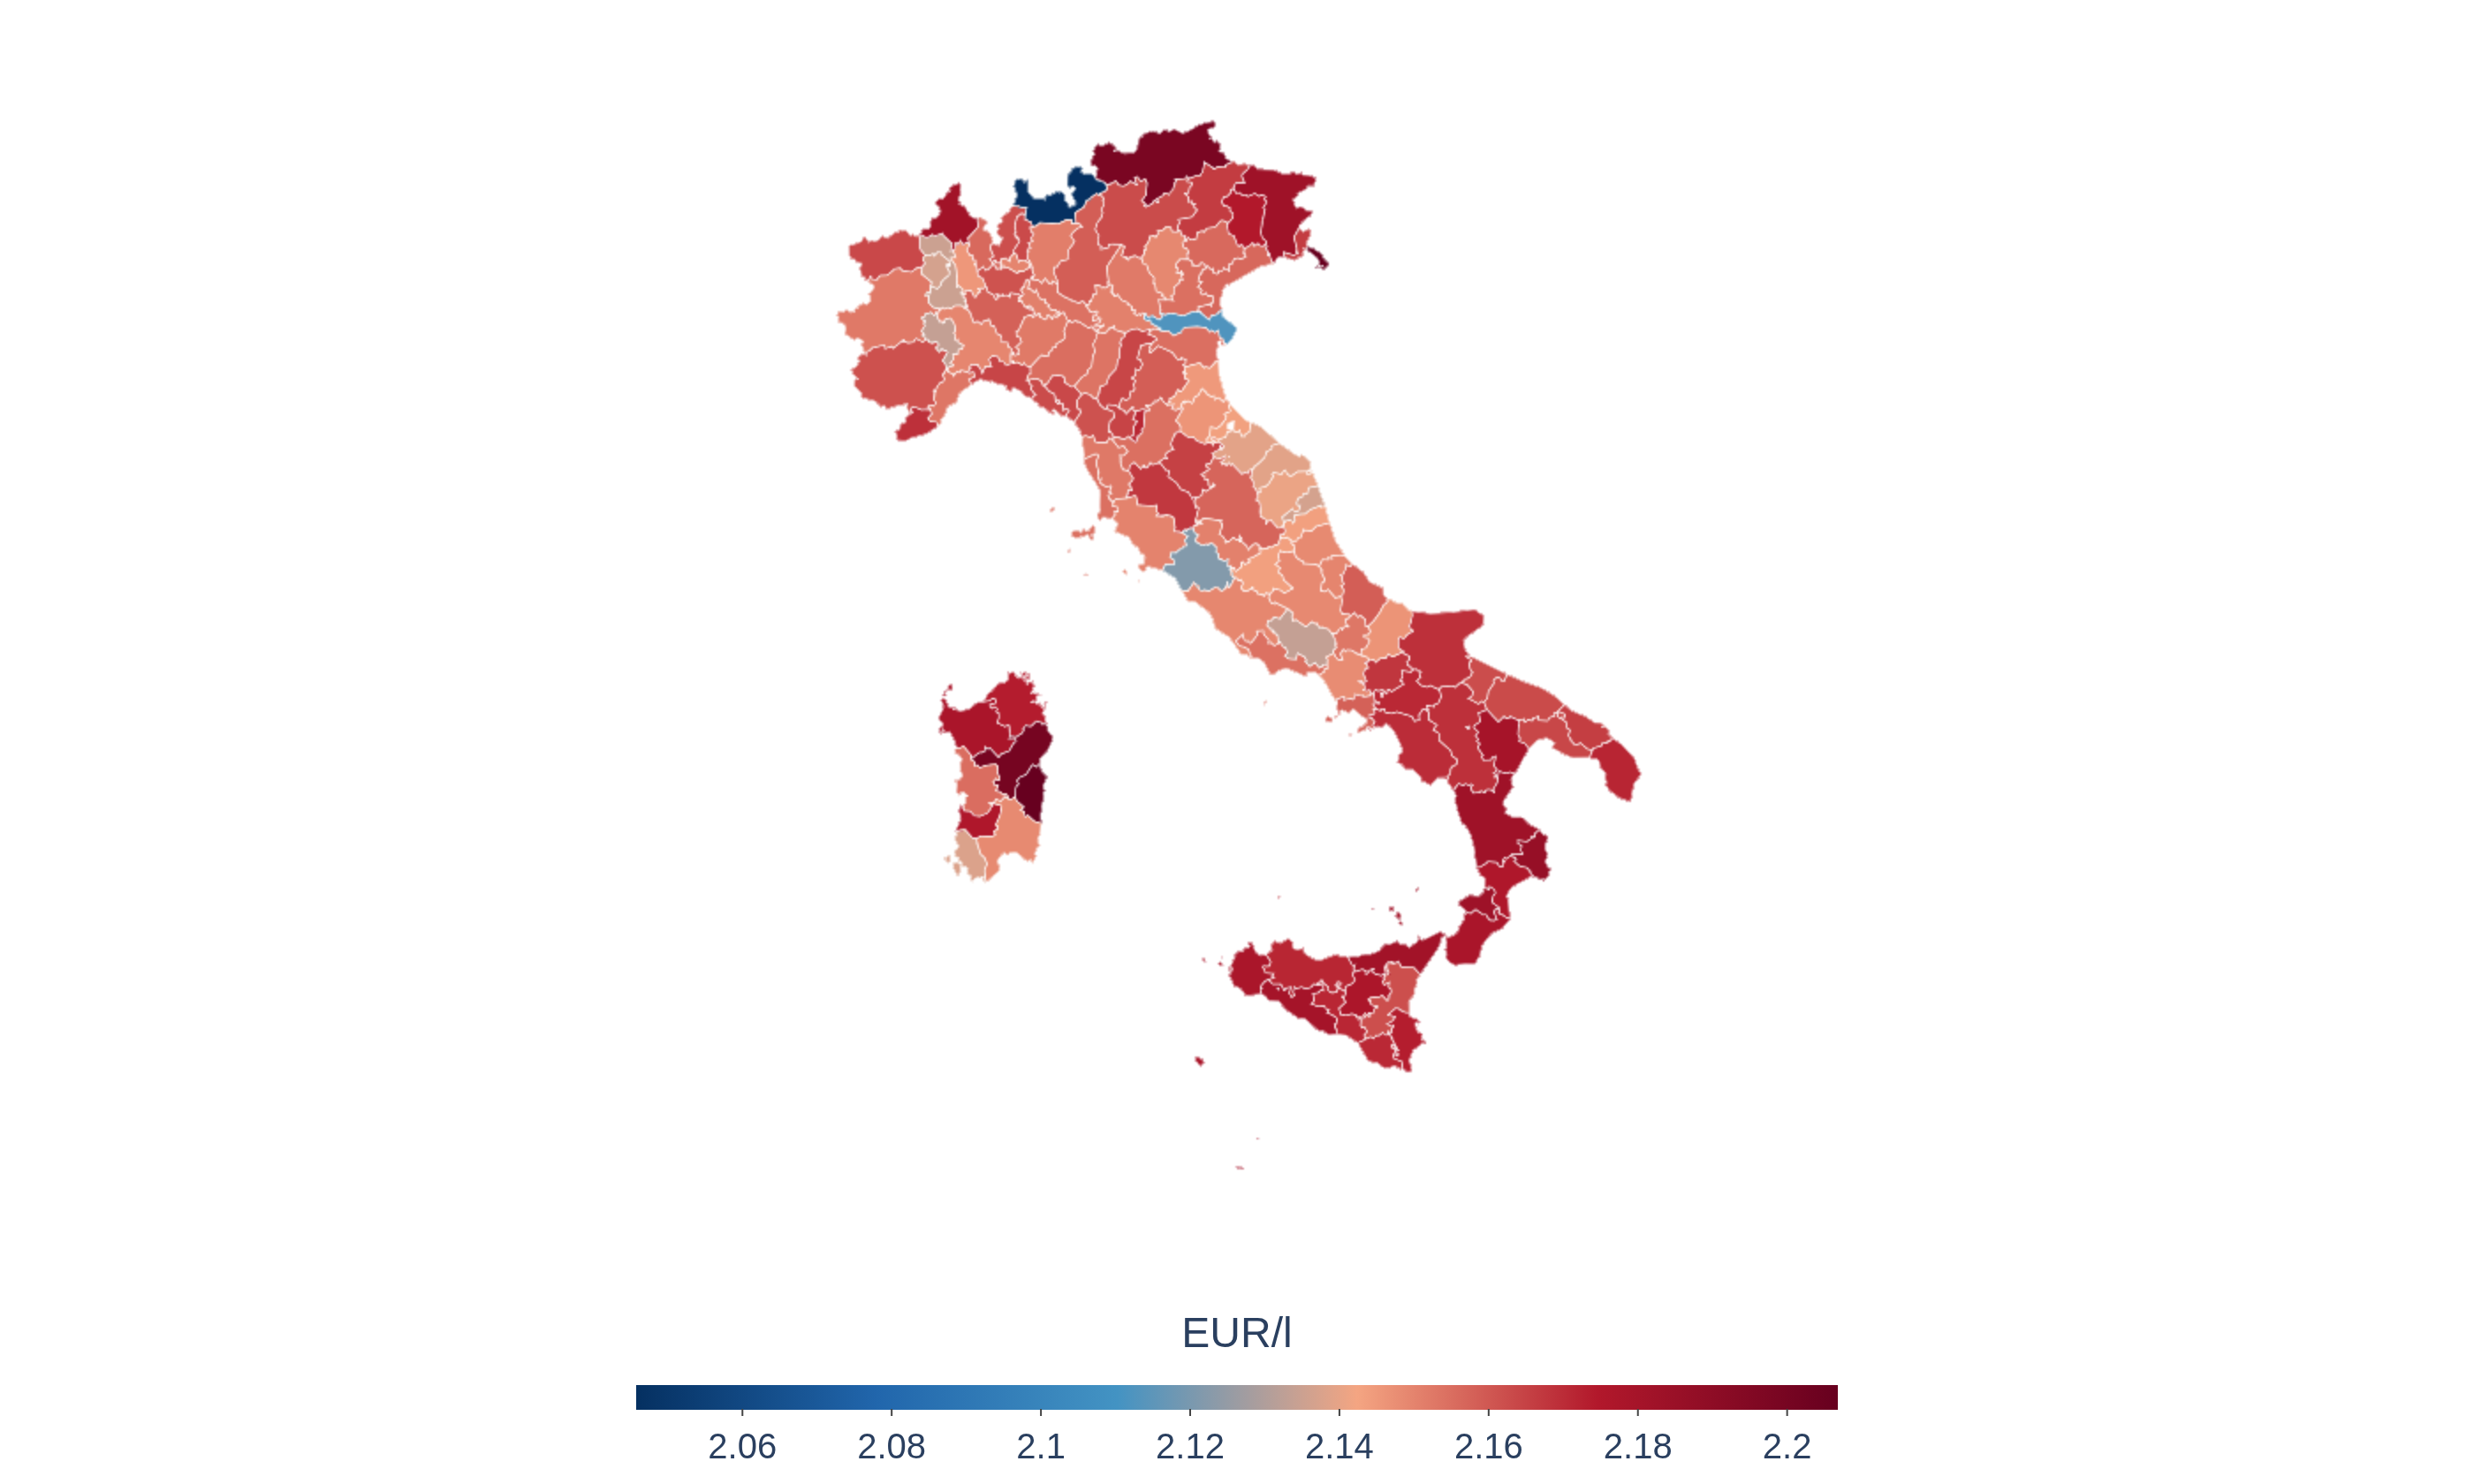
\includegraphics[width=0.8\textwidth]{output/figures/amap_price_pre_ben.png}
\caption{Petrol: mean provincial price, 27 September 2026 (\euro/l).}
\label{fig:ampreben}
\end{figure}

\begin{figure}[H]
\centering
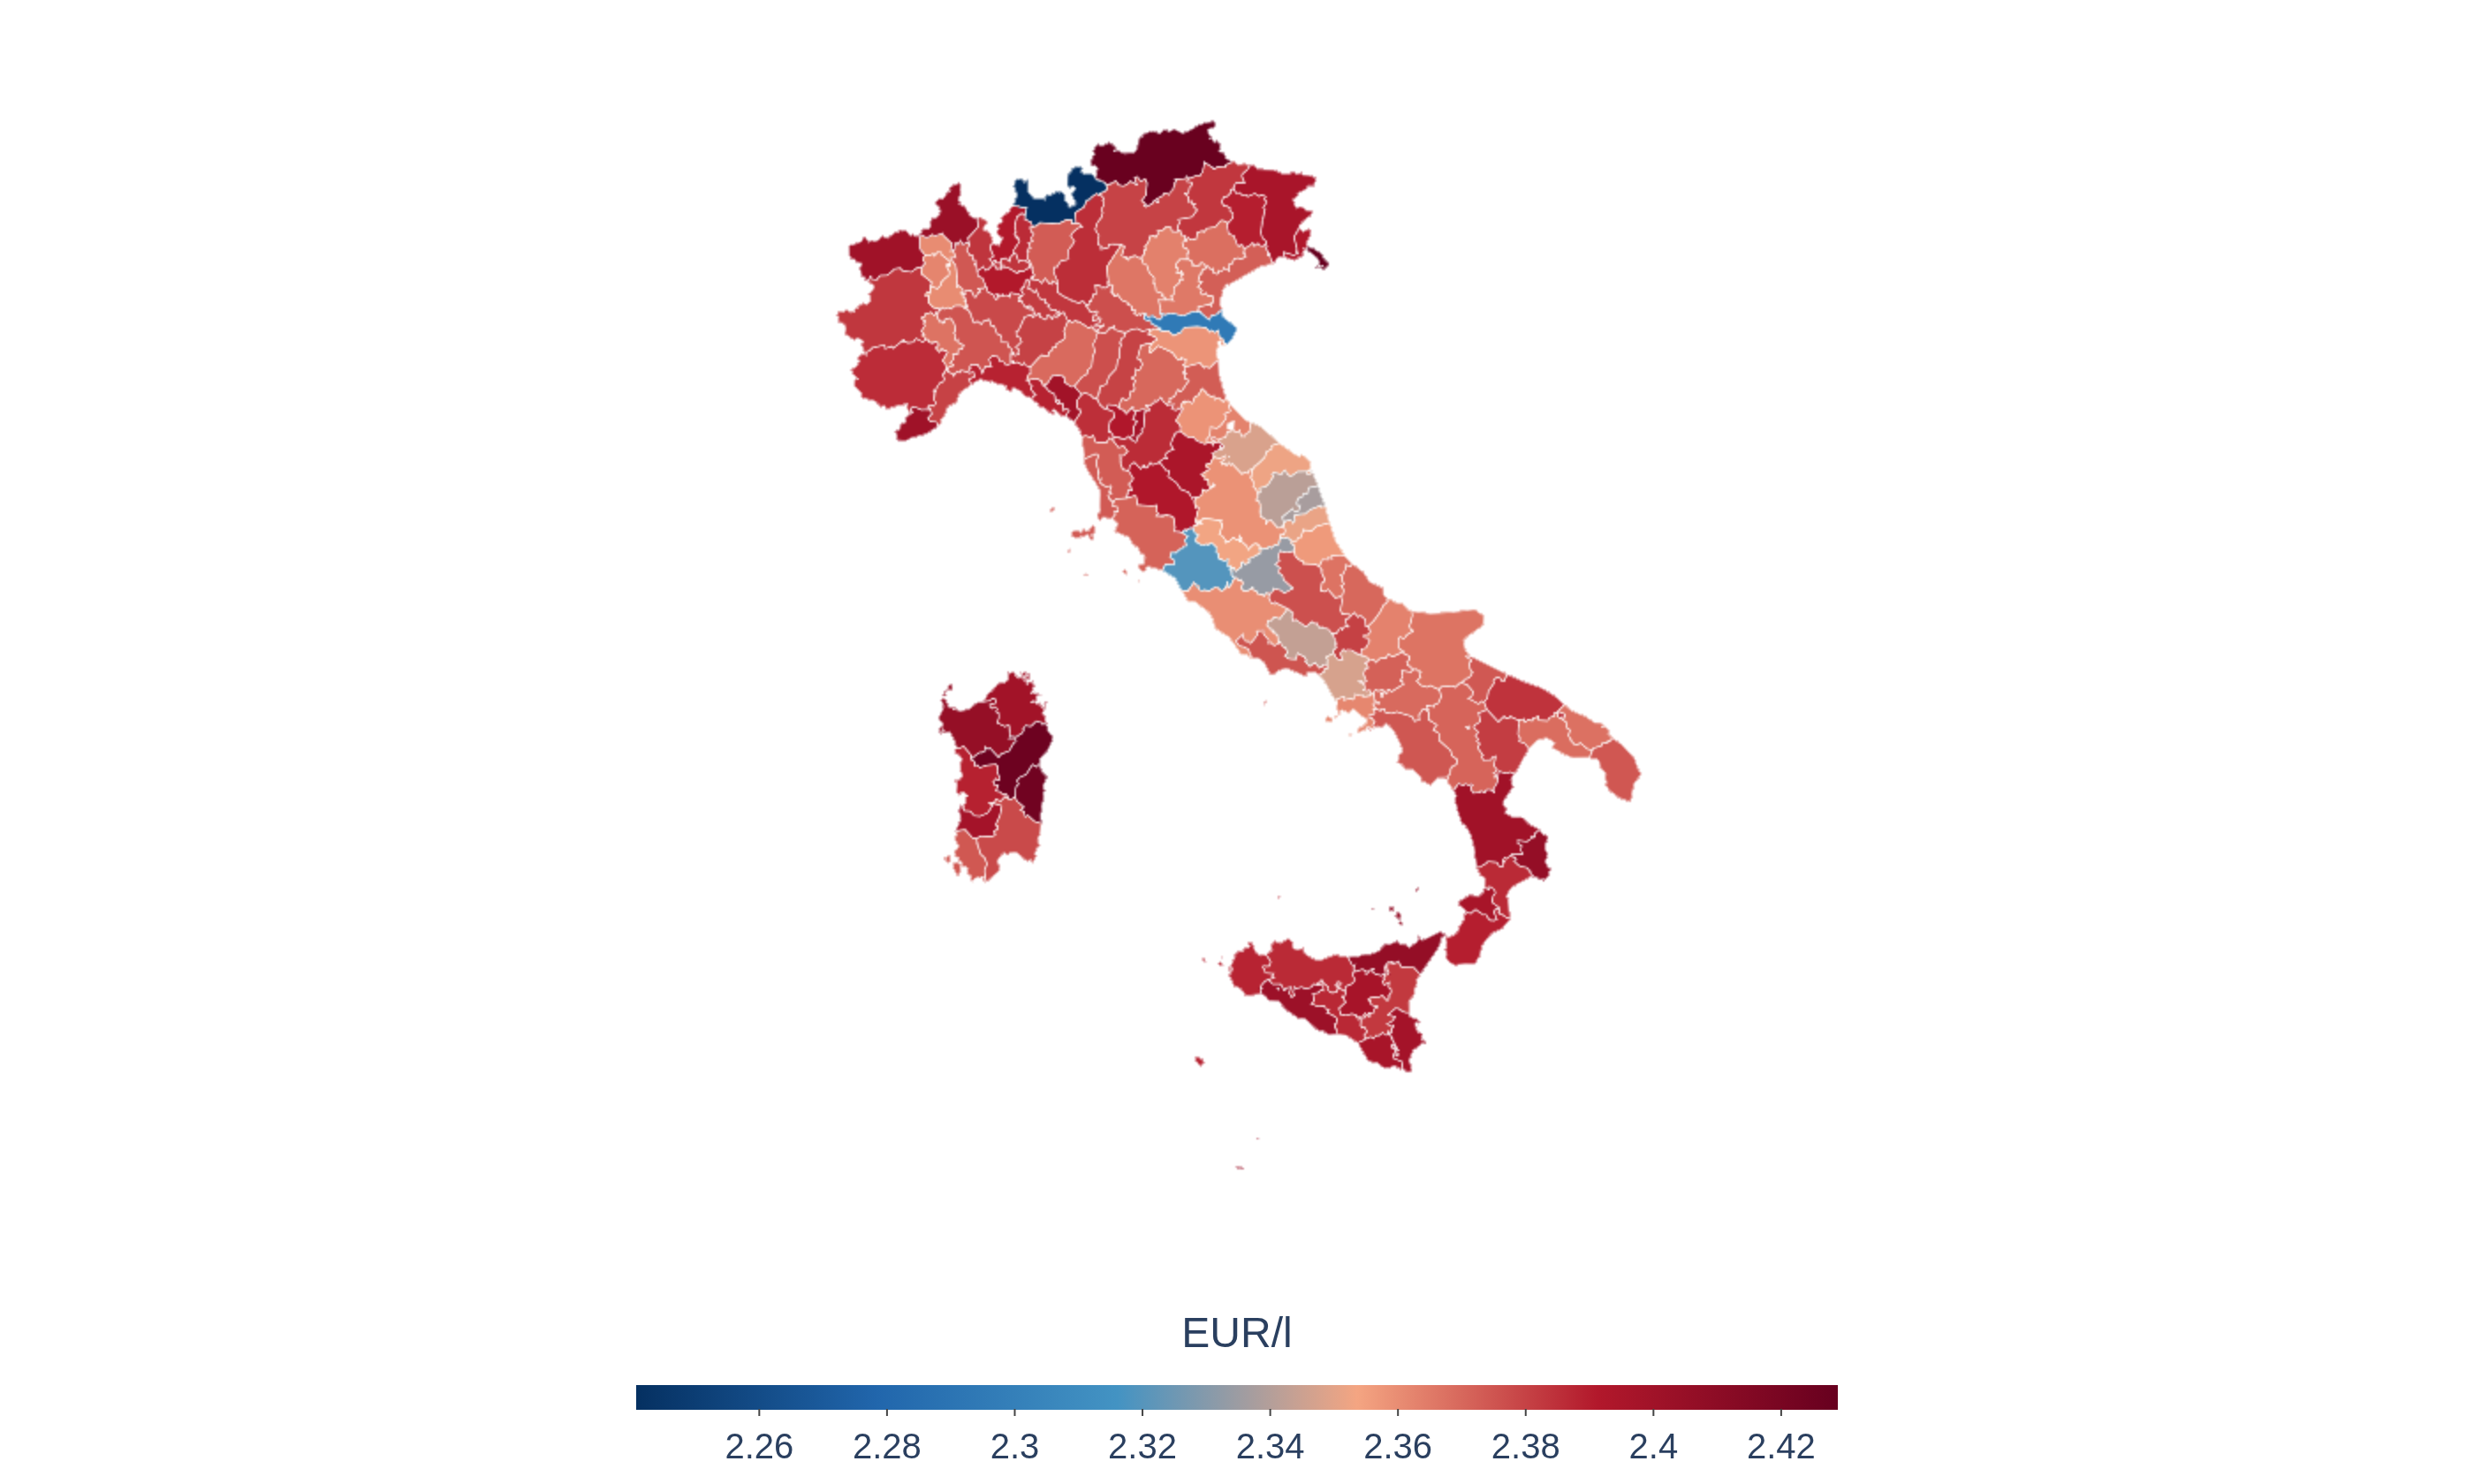
\includegraphics[width=0.8\textwidth]{output/figures/amap_price_pre_gas.png}
\caption{Diesel: mean provincial price, 27 September 2026 (\euro/l).}
\label{fig:ampregas}
\end{figure}

\clearpage
\paragraph{Average provincial price 7 days after the cap (5 October).}
Petrol collapses towards 2.00--2.10~\euro/l nearly everywhere; diesel
converges towards 2.10--2.30~\euro/l, with the reddest (highest)
provinces in the non-adopting fringes.

\begin{figure}[H]
\centering
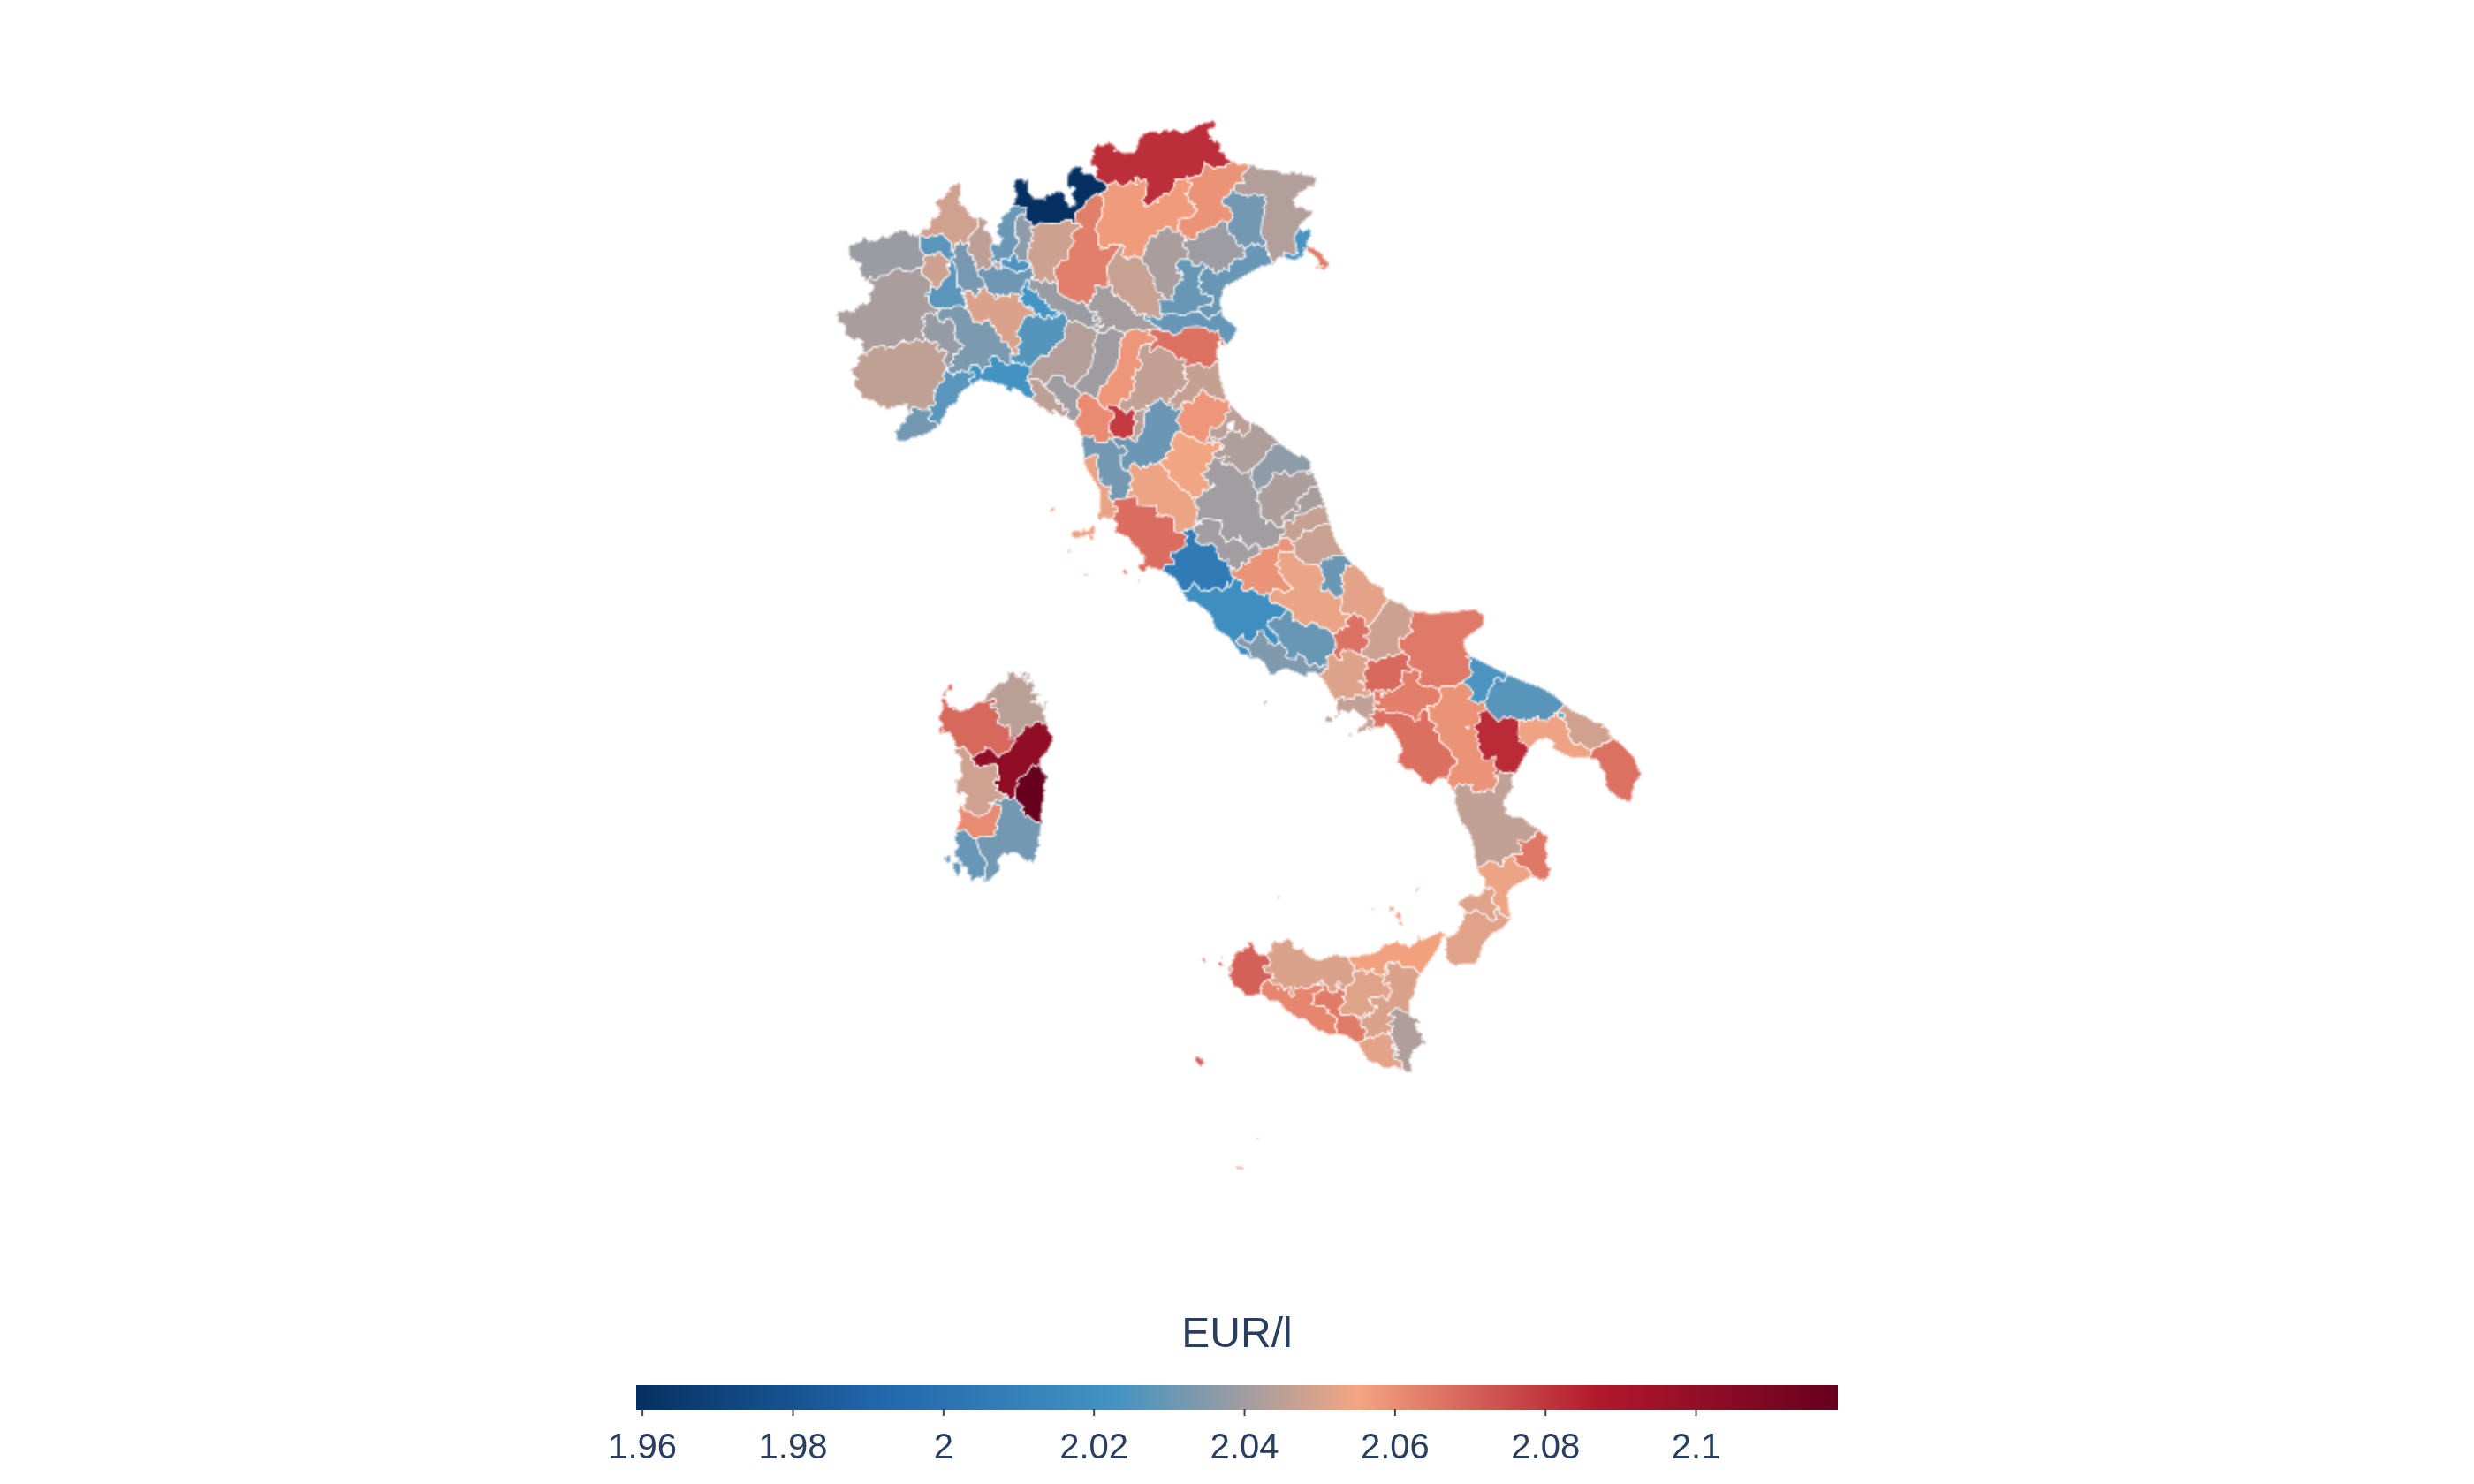
\includegraphics[width=0.8\textwidth]{output/figures/amap_price_post7_ben.png}
\caption{Petrol: mean provincial price, 5 October 2026 (\euro/l).}
\label{fig:ampostben}
\end{figure}

\begin{figure}[H]
\centering
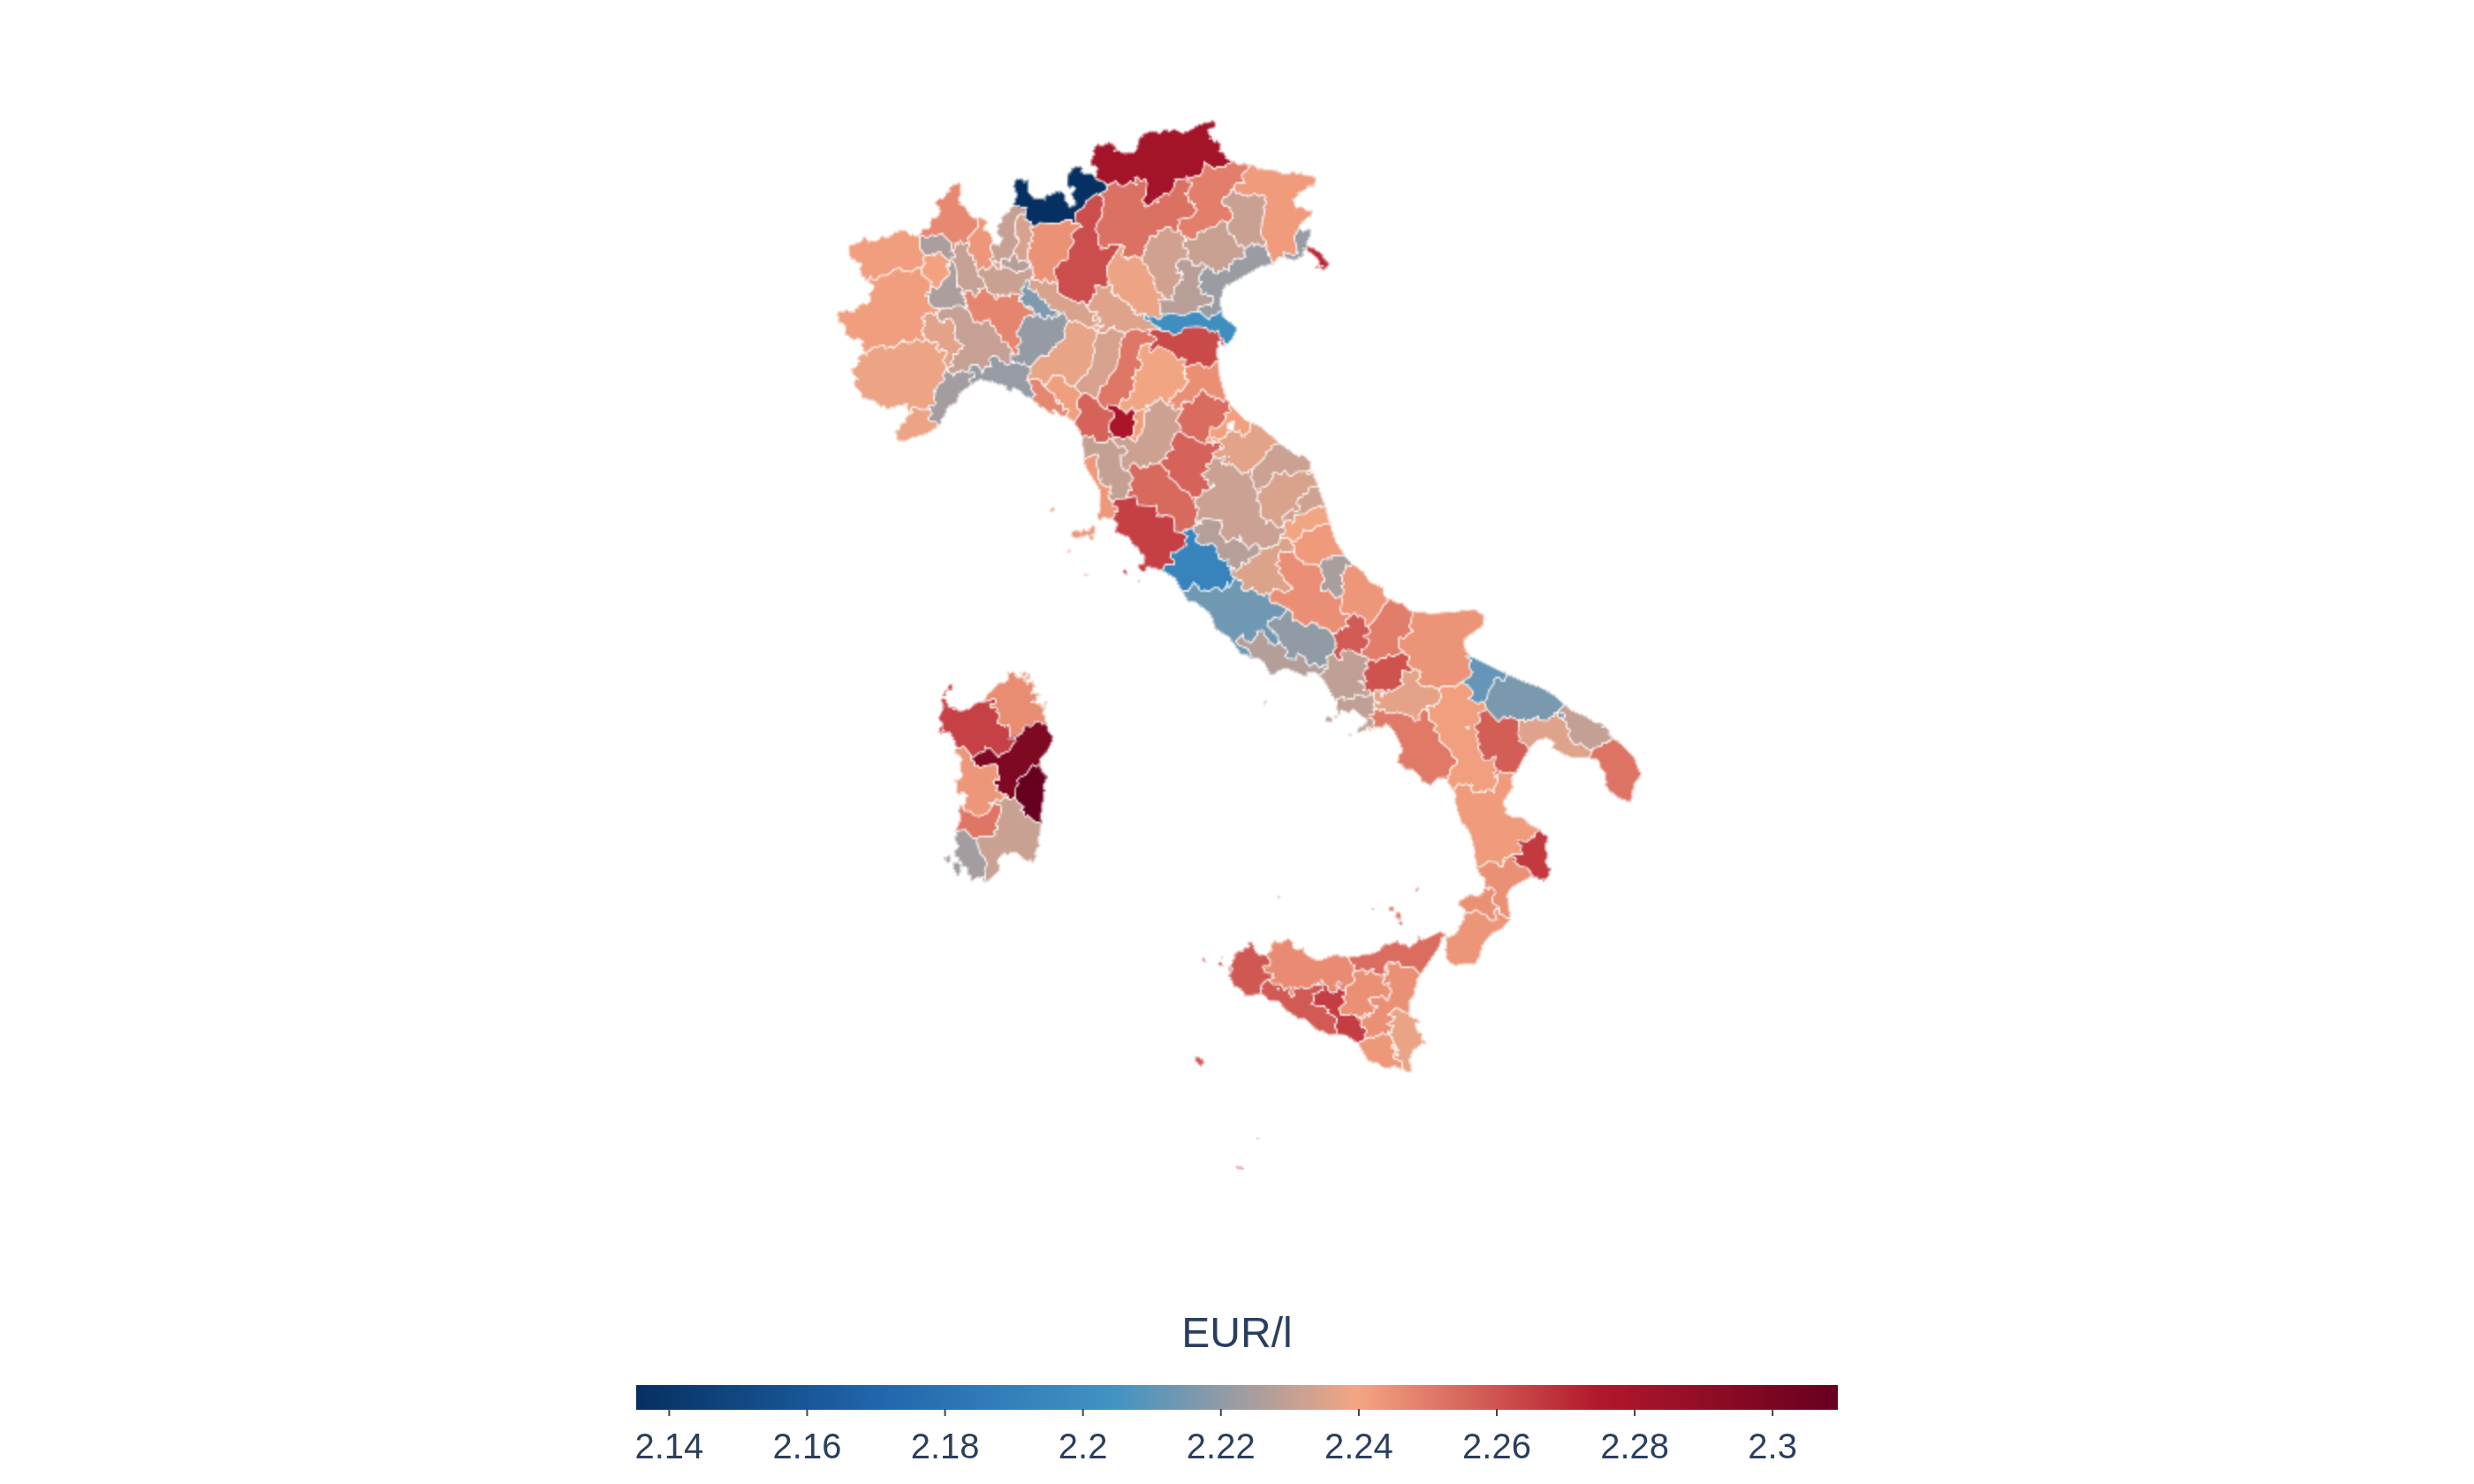
\includegraphics[width=0.8\textwidth]{output/figures/amap_price_post7_gas.png}
\caption{Diesel: mean provincial price, 5 October 2026 (\euro/l).}
\label{fig:ampostgas}
\end{figure}

\clearpage
\paragraph{Price gap between future non-adopters and adopters before
the cap (21--27 September).} Even before the cap, stations that would
never adopt priced above those that would, by up to 200~c/l (petrol)
and 217~c/l (diesel) in the reddest provinces --- pre-cap selection,
not just post-cap repricing.

\begin{figure}[H]
\centering
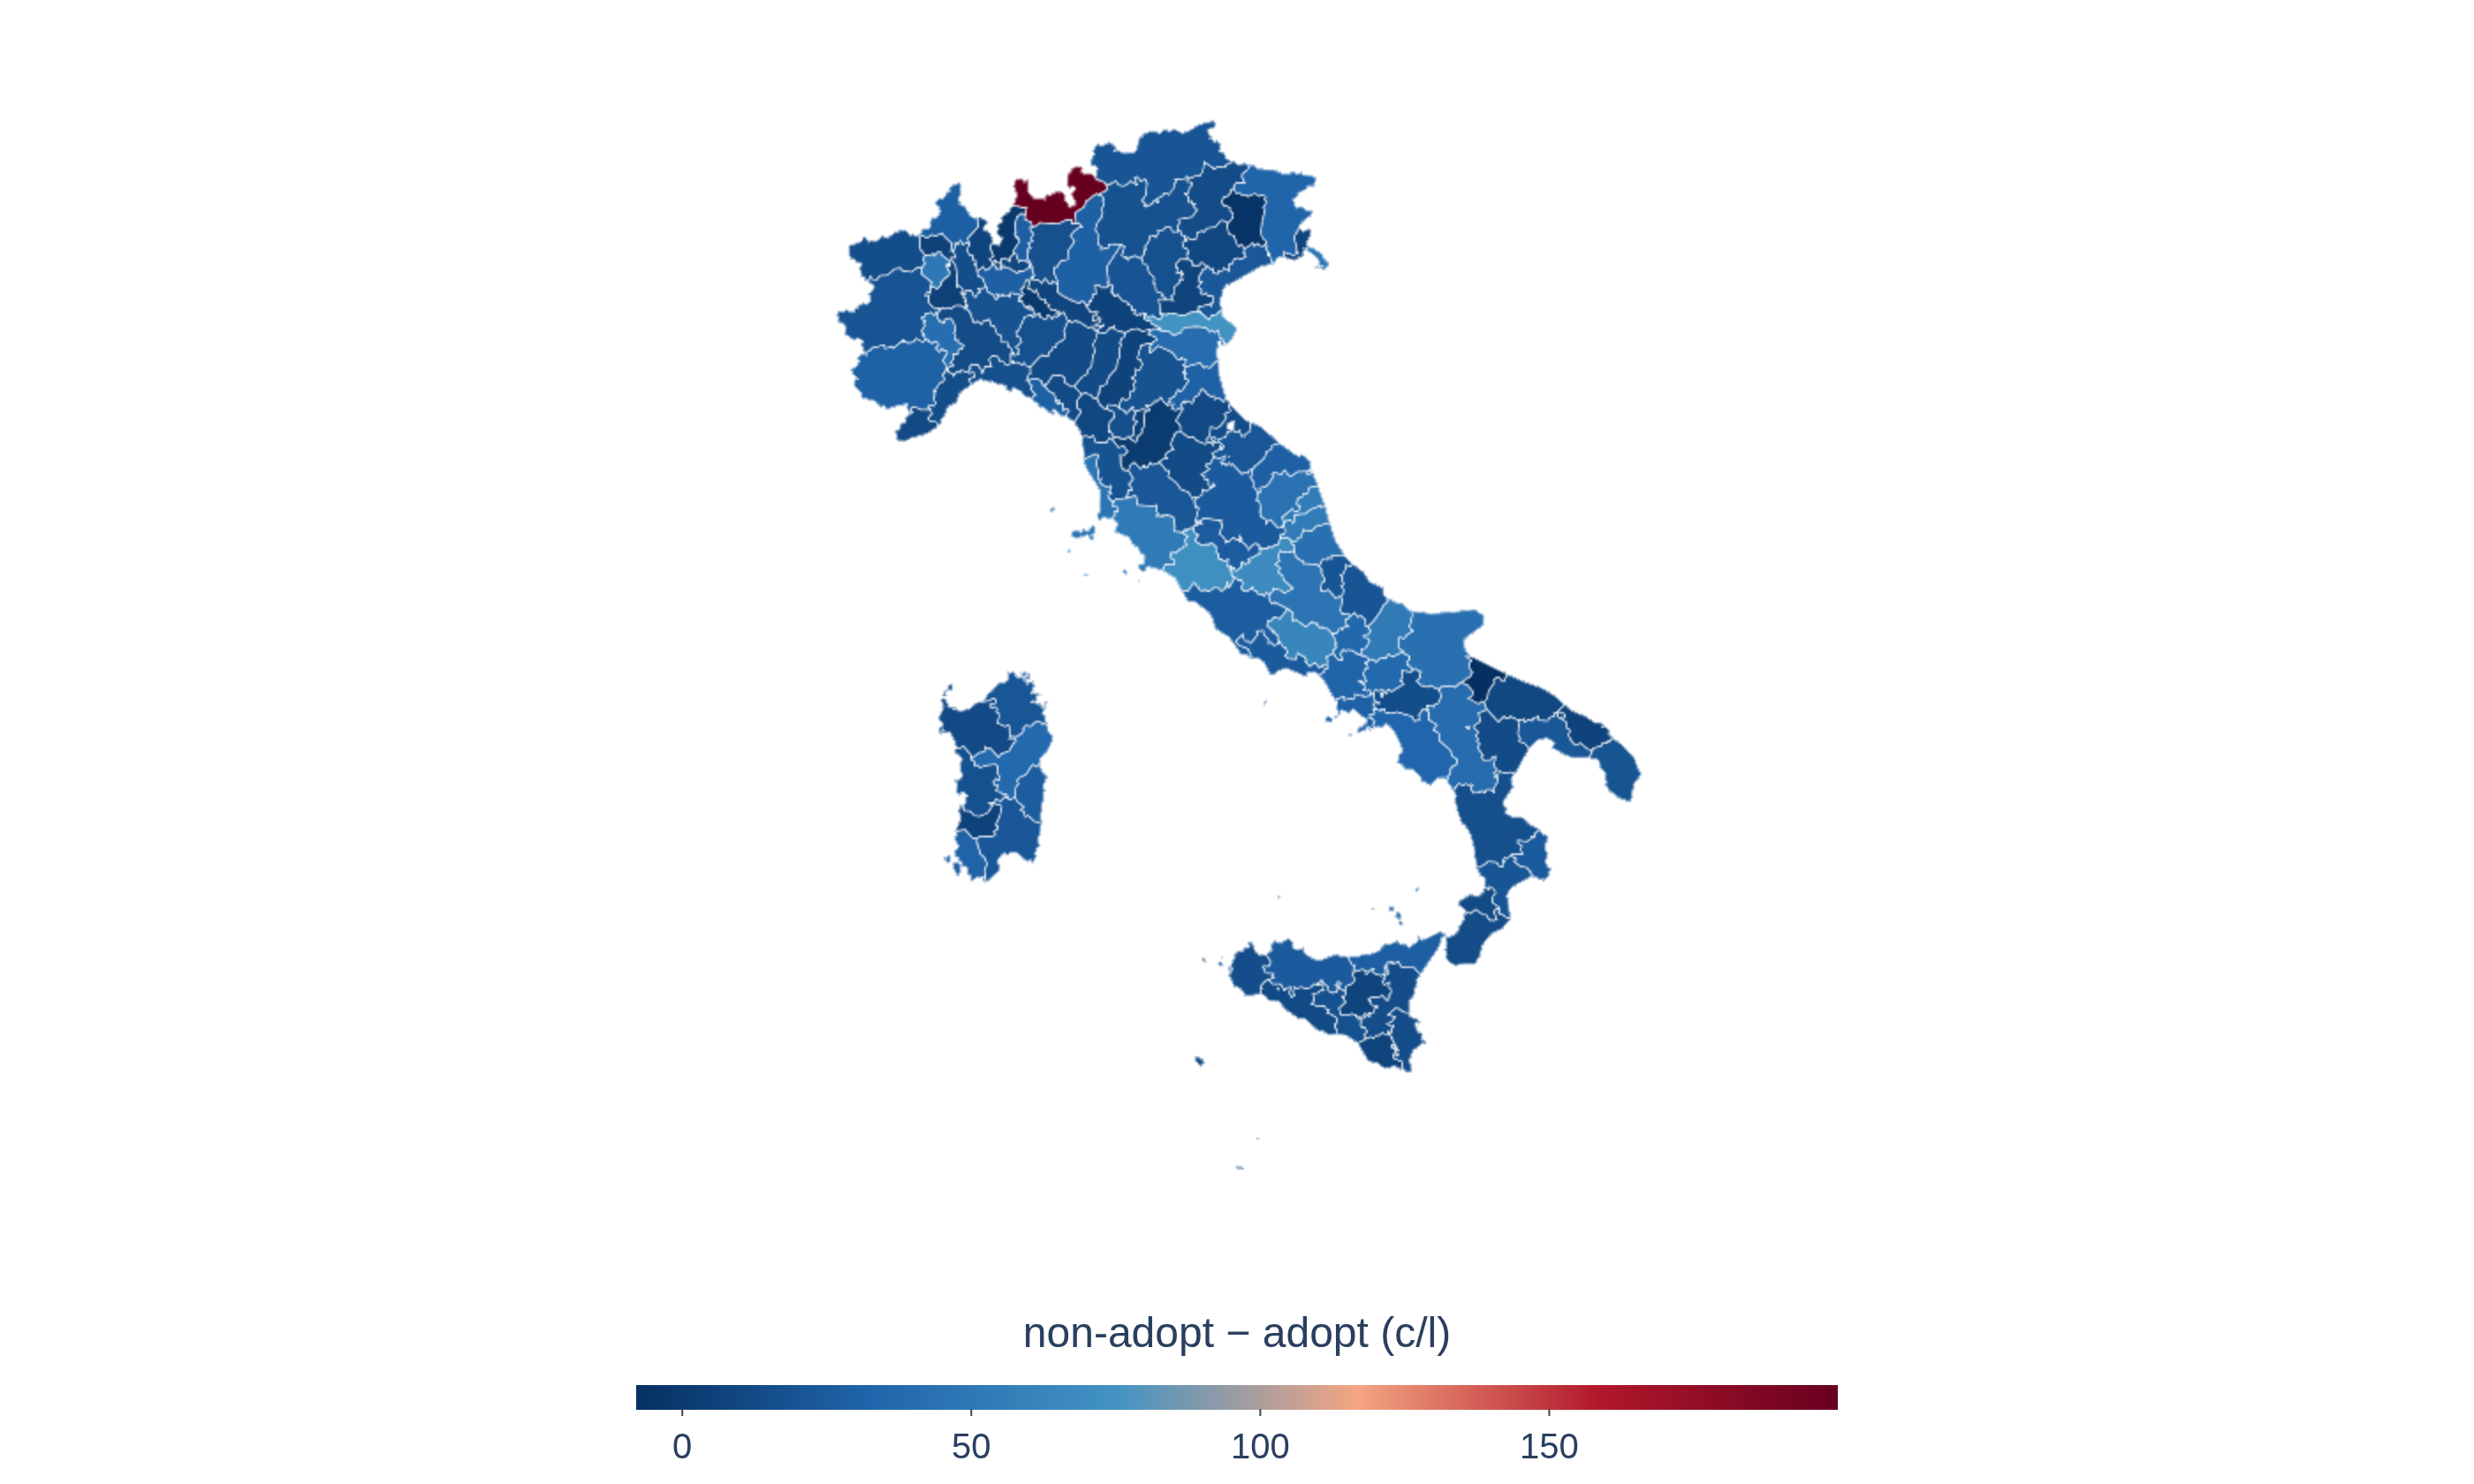
\includegraphics[width=0.8\textwidth]{output/figures/amap_gappre_ben.png}
\caption{Petrol: pre-cap mean price of non-adopters minus adopters
(c/l).}
\label{fig:amgappreben}
\end{figure}

\begin{figure}[H]
\centering
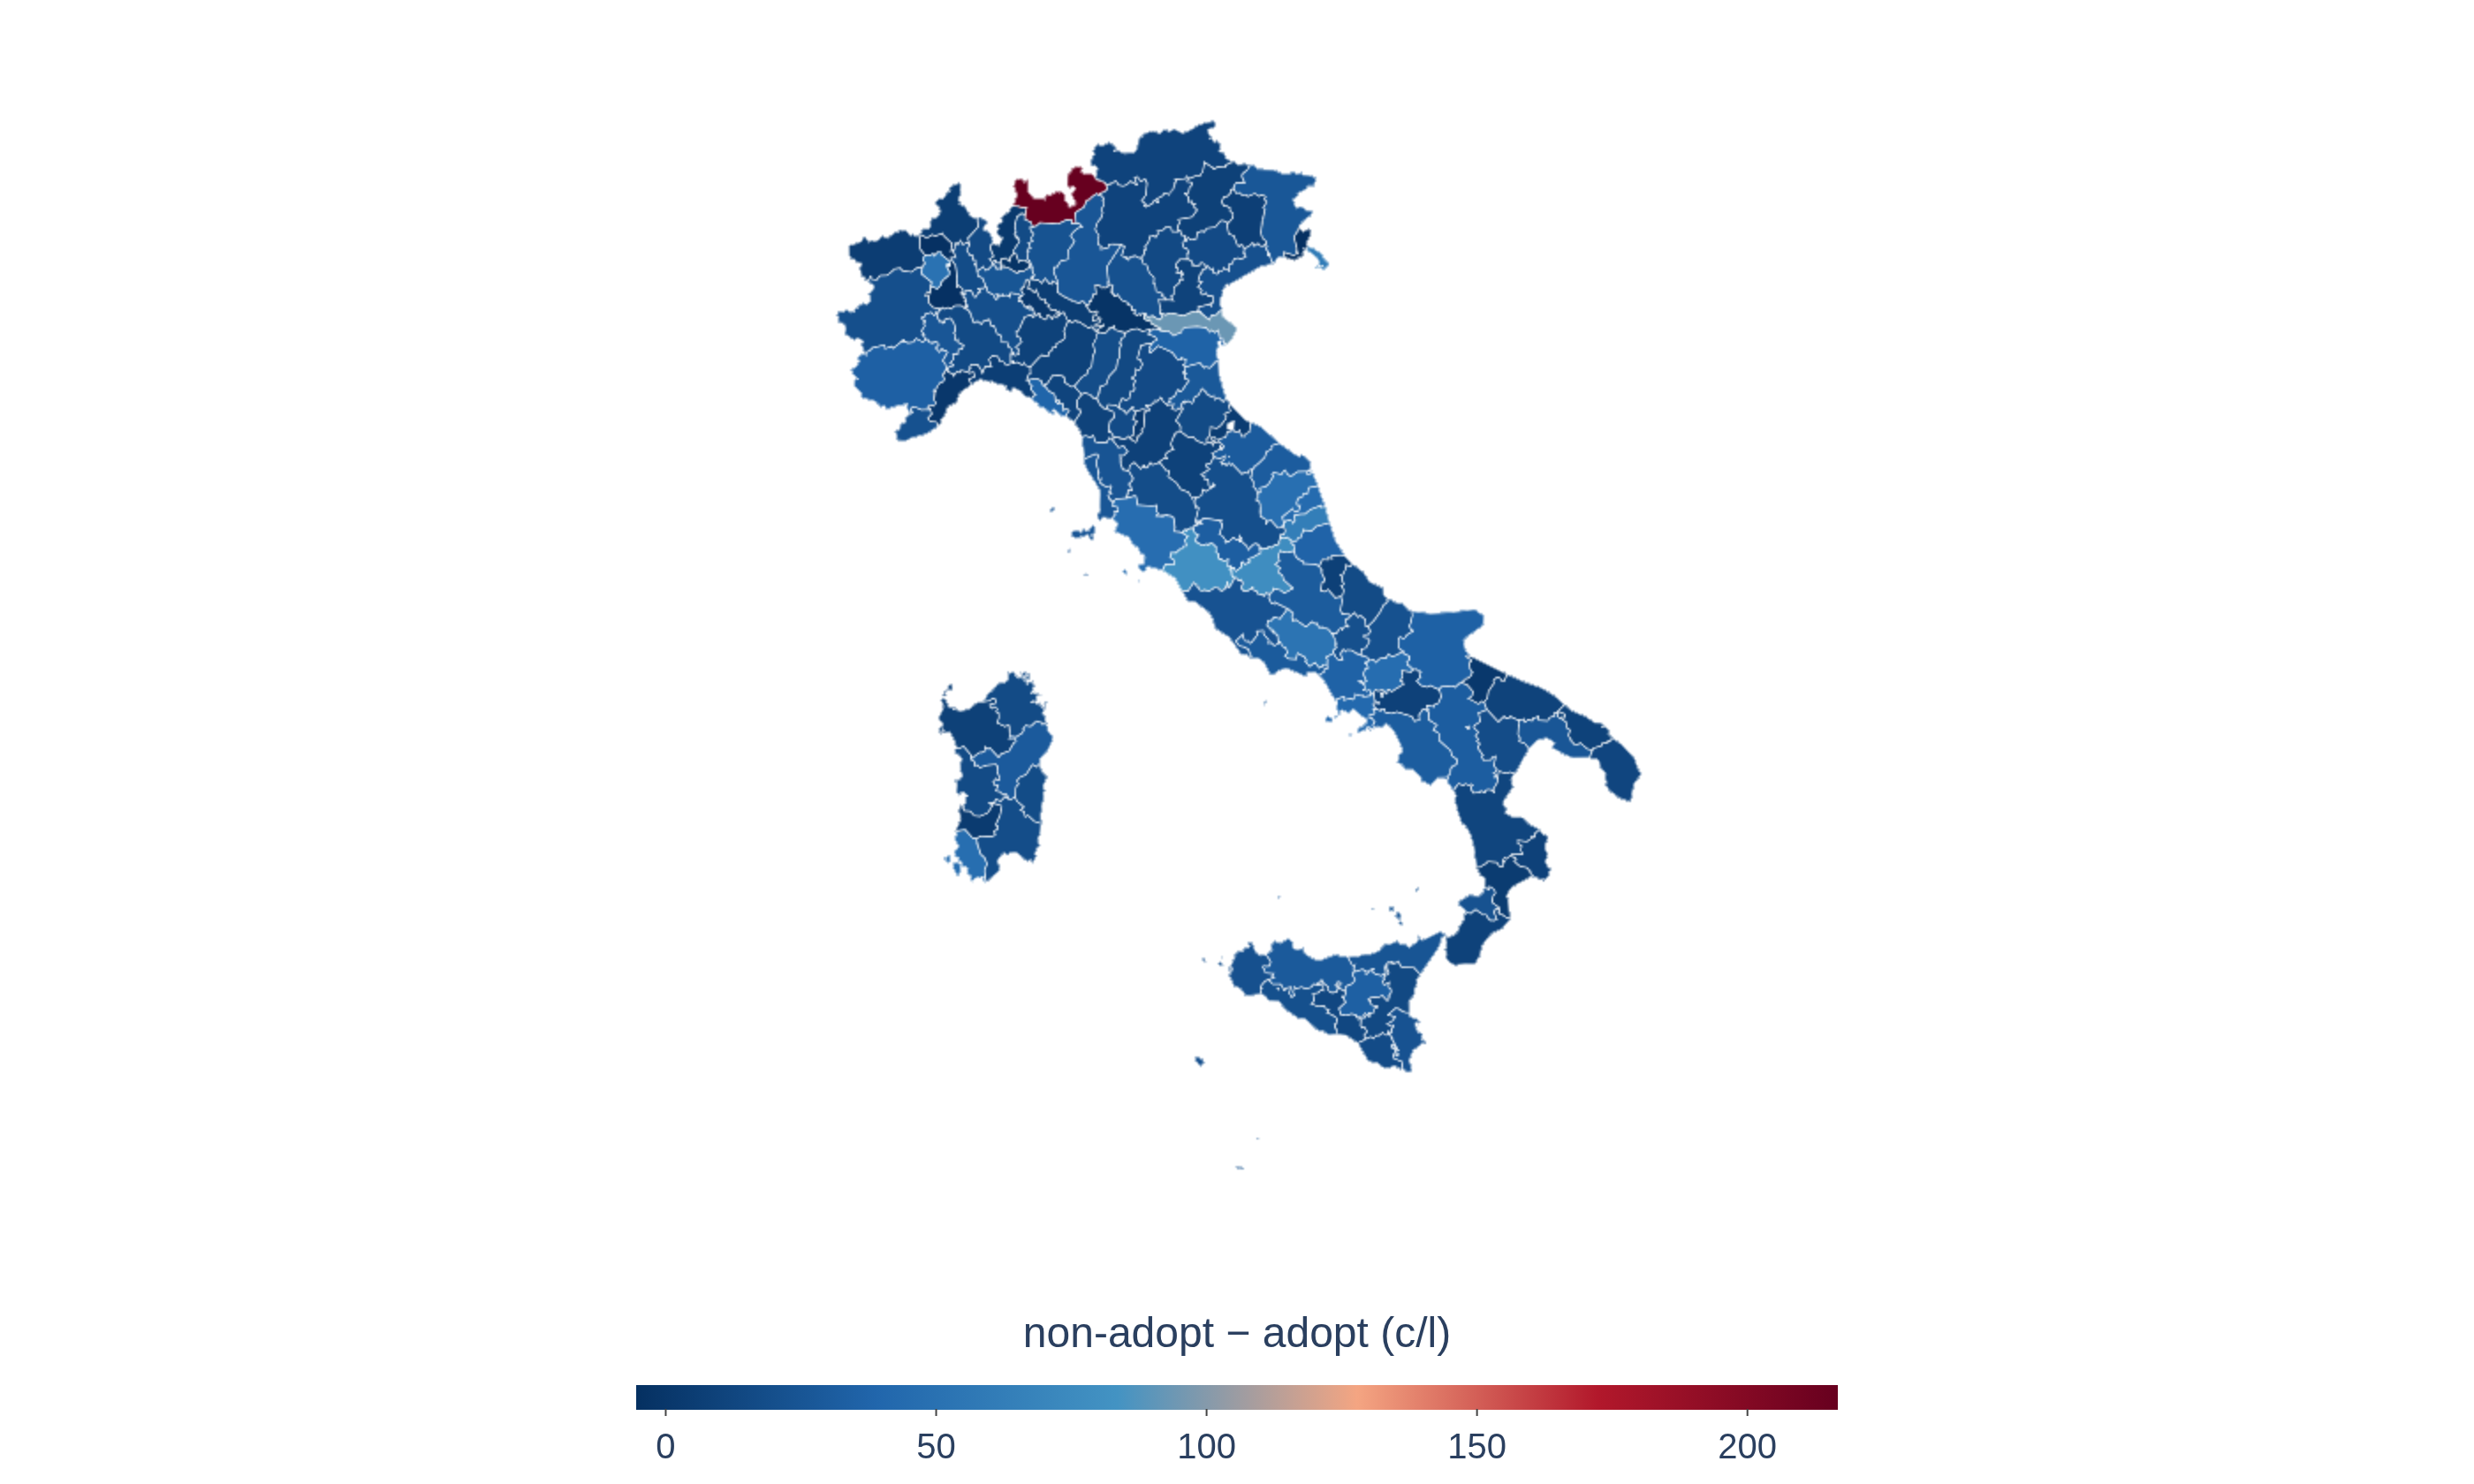
\includegraphics[width=0.8\textwidth]{output/figures/amap_gappre_gas.png}
\caption{Diesel: pre-cap mean price of non-adopters minus adopters
(c/l).}
\label{fig:amgappregas}
\end{figure}

\paragraph{Post-cap price gap between non-adopters and adopters
(28 September -- 7 October).} Non-adopters price above adopters in
every province, by 56--263~c/l (petrol) and 60--282~c/l (diesel); the
gap is reddest (widest) where adoption was high and the provincial mean
is anchored at the cap.

\begin{figure}[H]
\centering
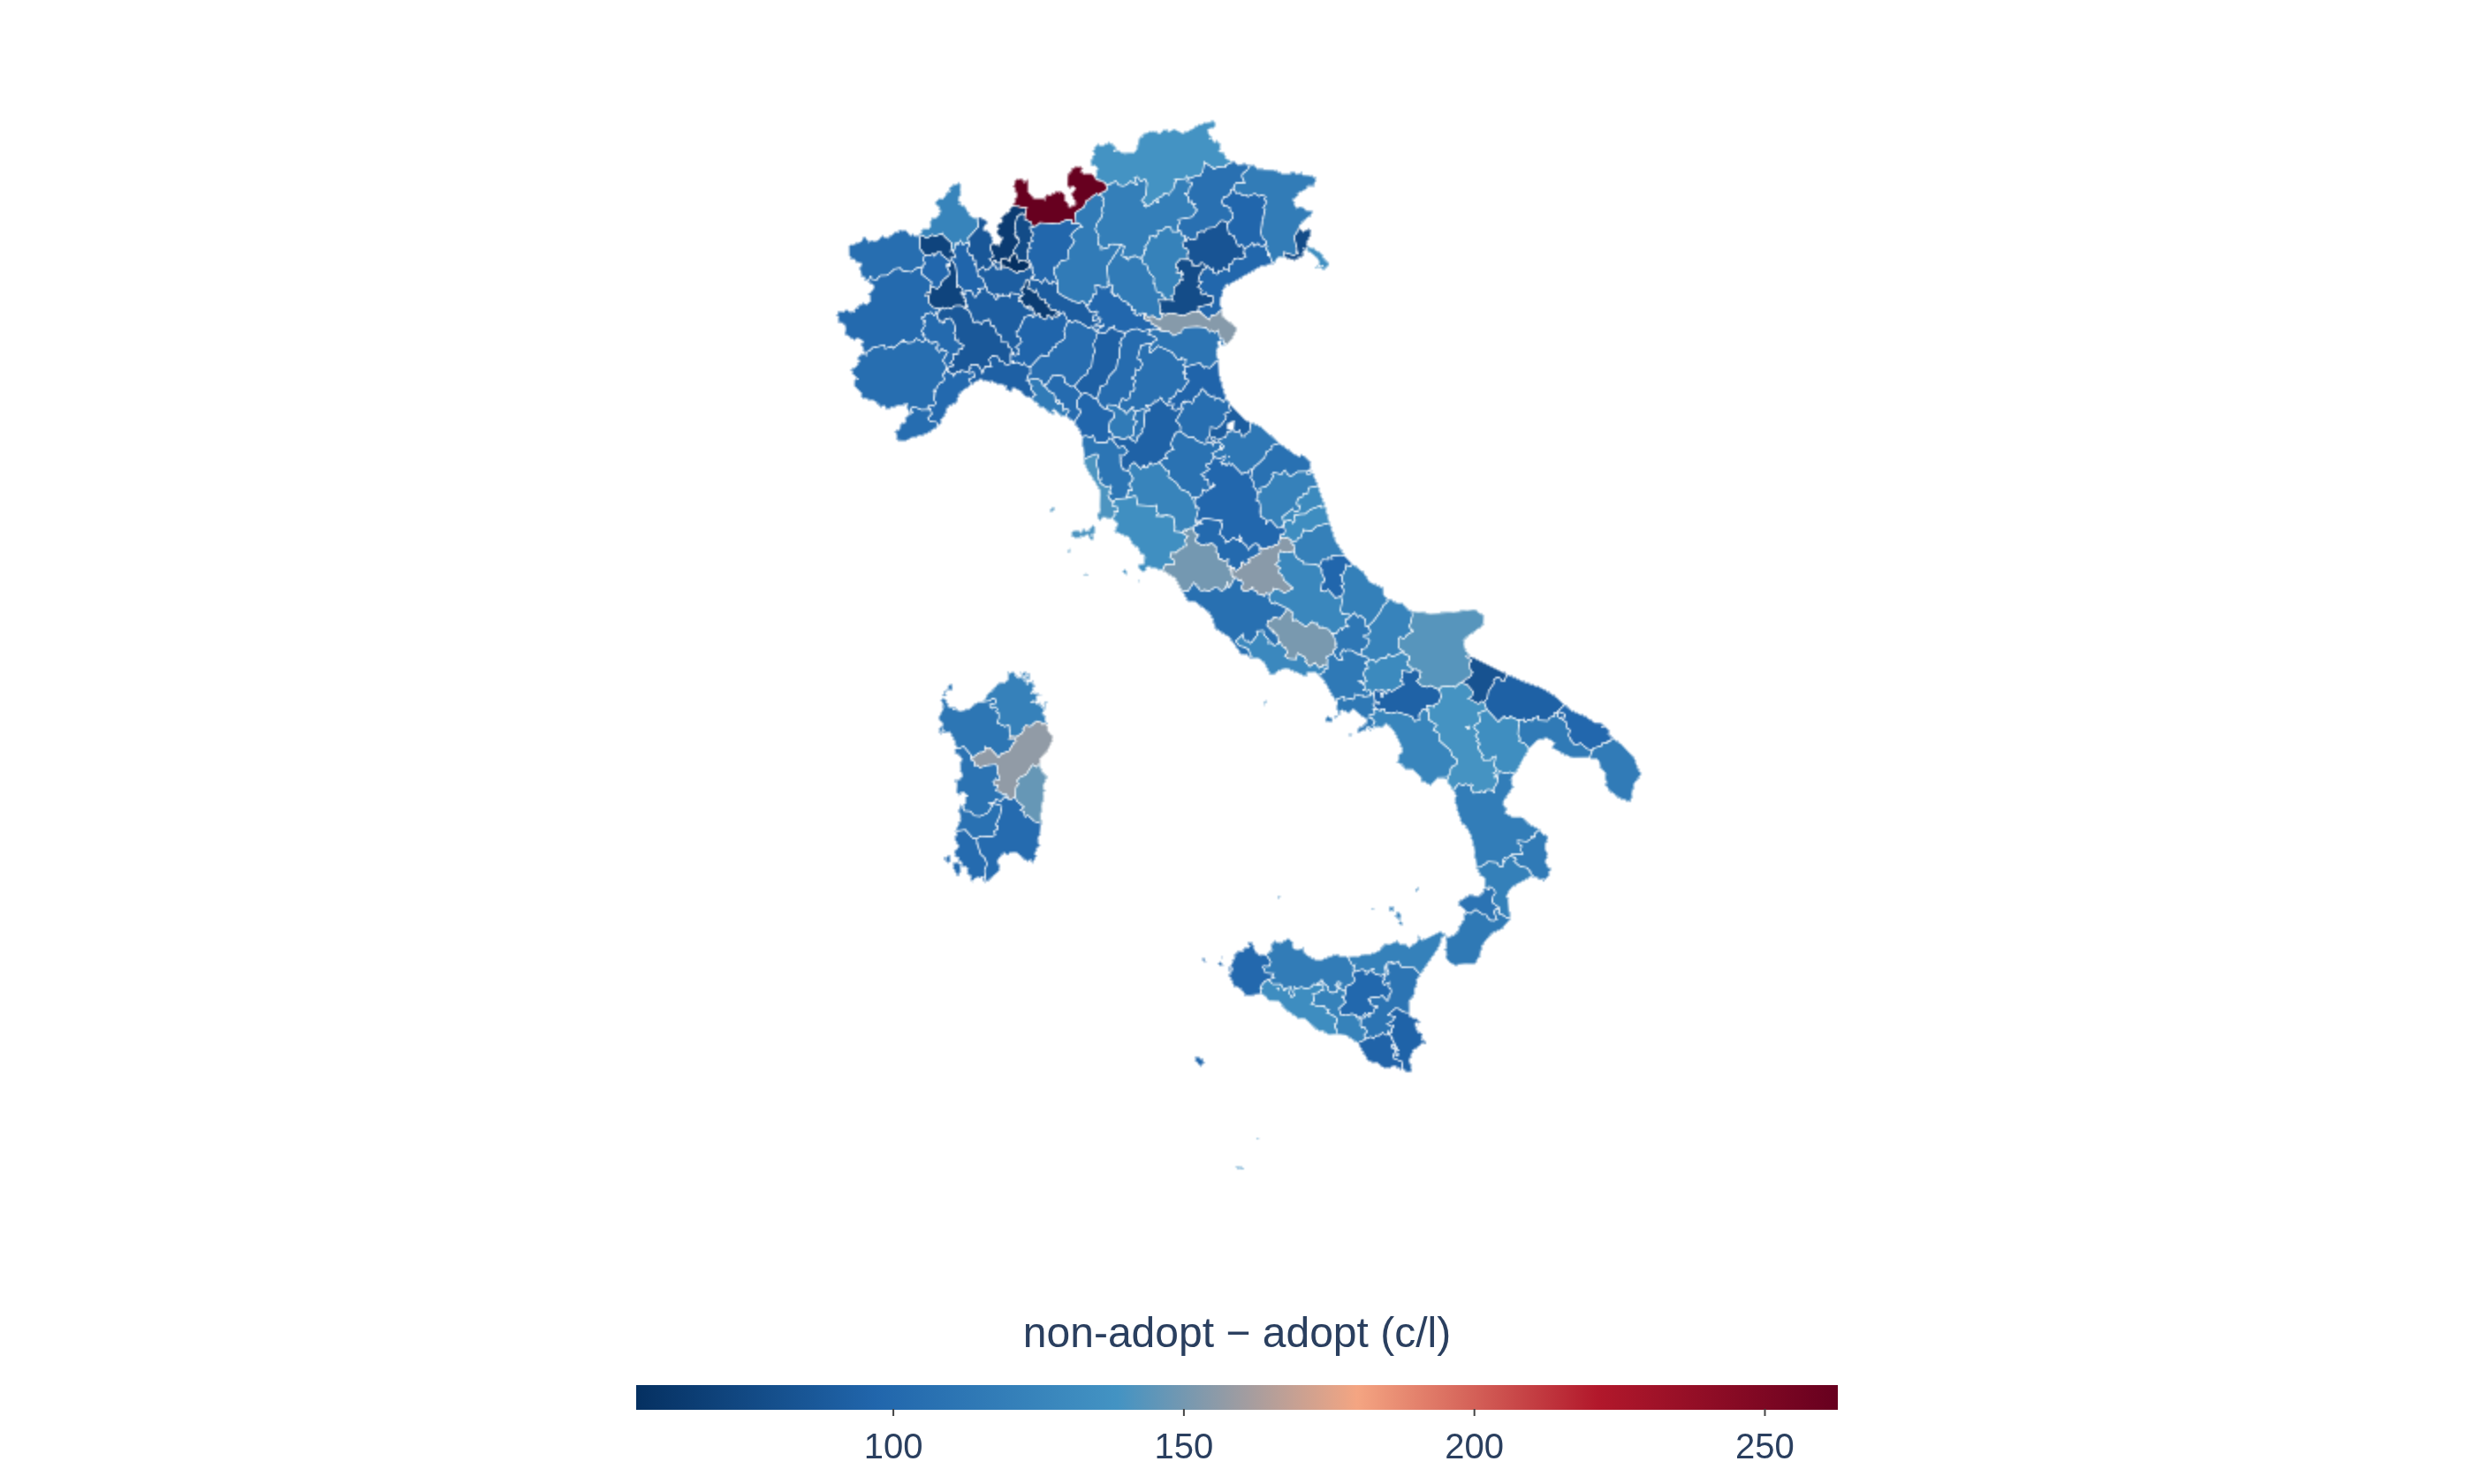
\includegraphics[width=0.8\textwidth]{output/figures/amap_gapadoption_ben.png}
\caption{Petrol: mean post-cap price of non-adopters minus adopters
(c/l).}
\label{fig:amgapben}
\end{figure}

\begin{figure}[H]
\centering
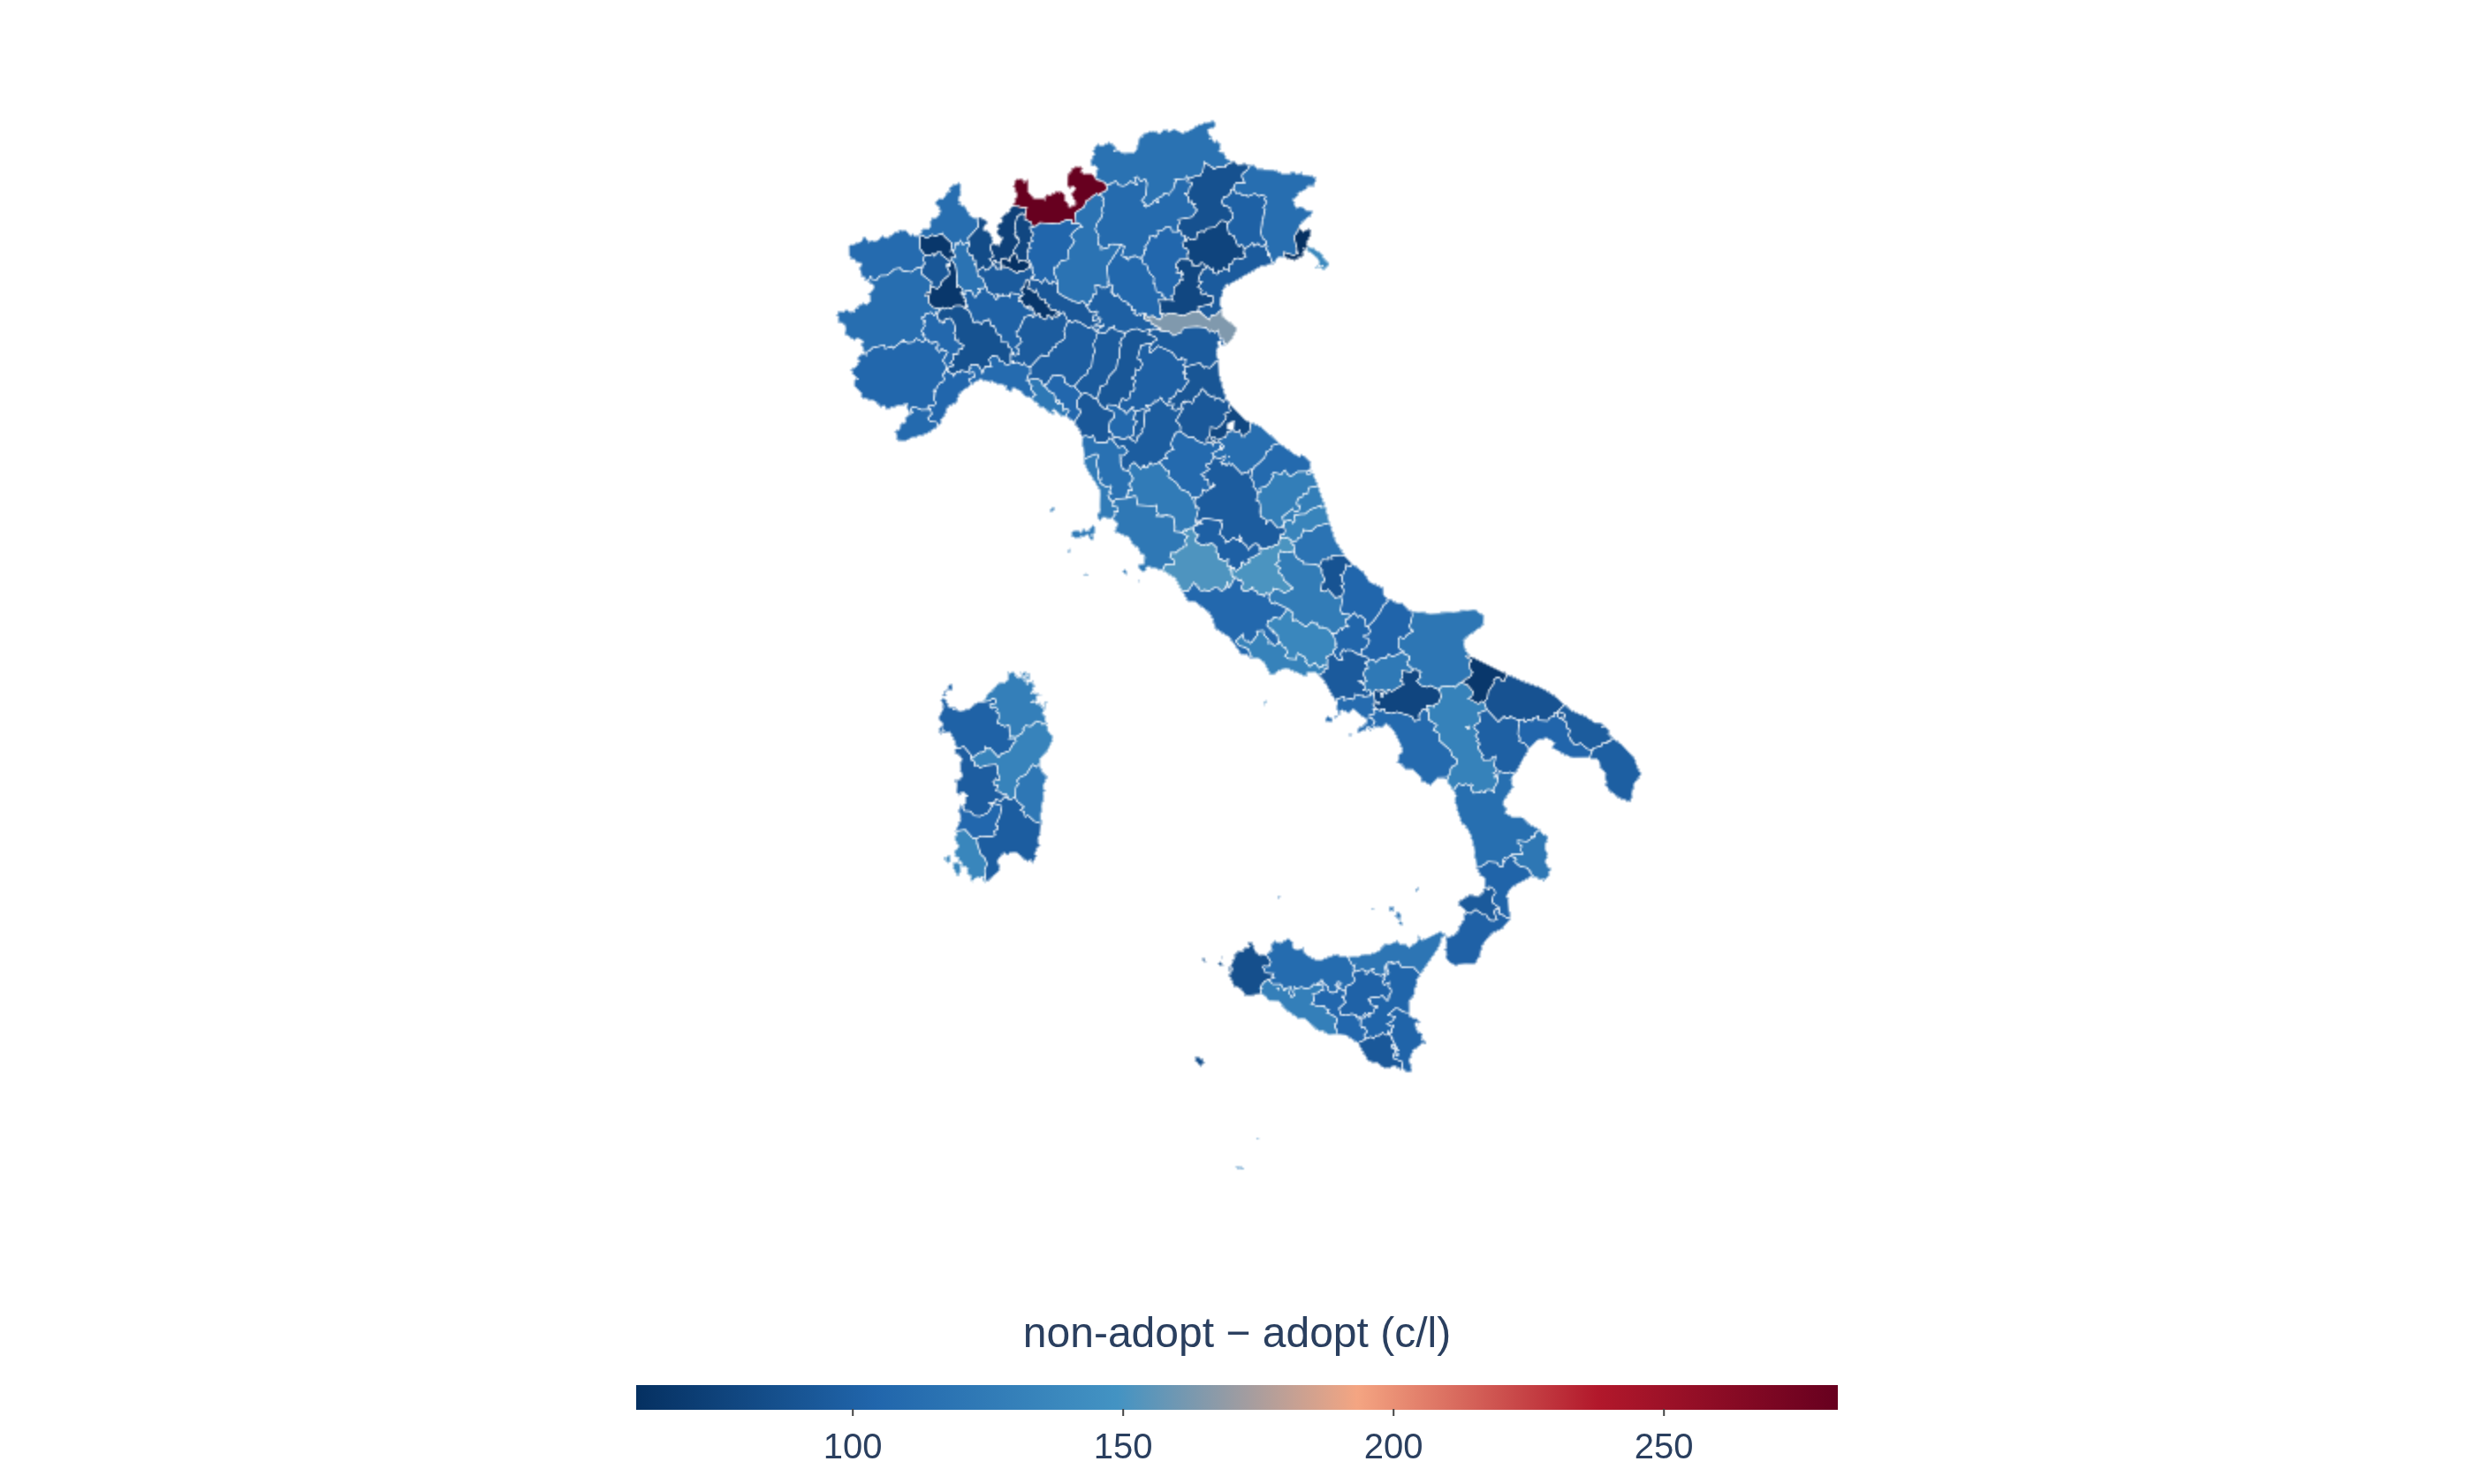
\includegraphics[width=0.8\textwidth]{output/figures/amap_gapadoption_gas.png}
\caption{Diesel: mean post-cap price of non-adopters minus adopters
(c/l).}
\label{fig:amgapgas}
\end{figure}

\clearpage
\paragraph{Share of cap adopters 7 days after the cap.} Adoption
spans 32--74\% of units across provinces in both fuels, with the
reddest provinces concentrated in the central-northern corridors
identified in \cref{fig:mapall}.

\begin{figure}[H]
\centering
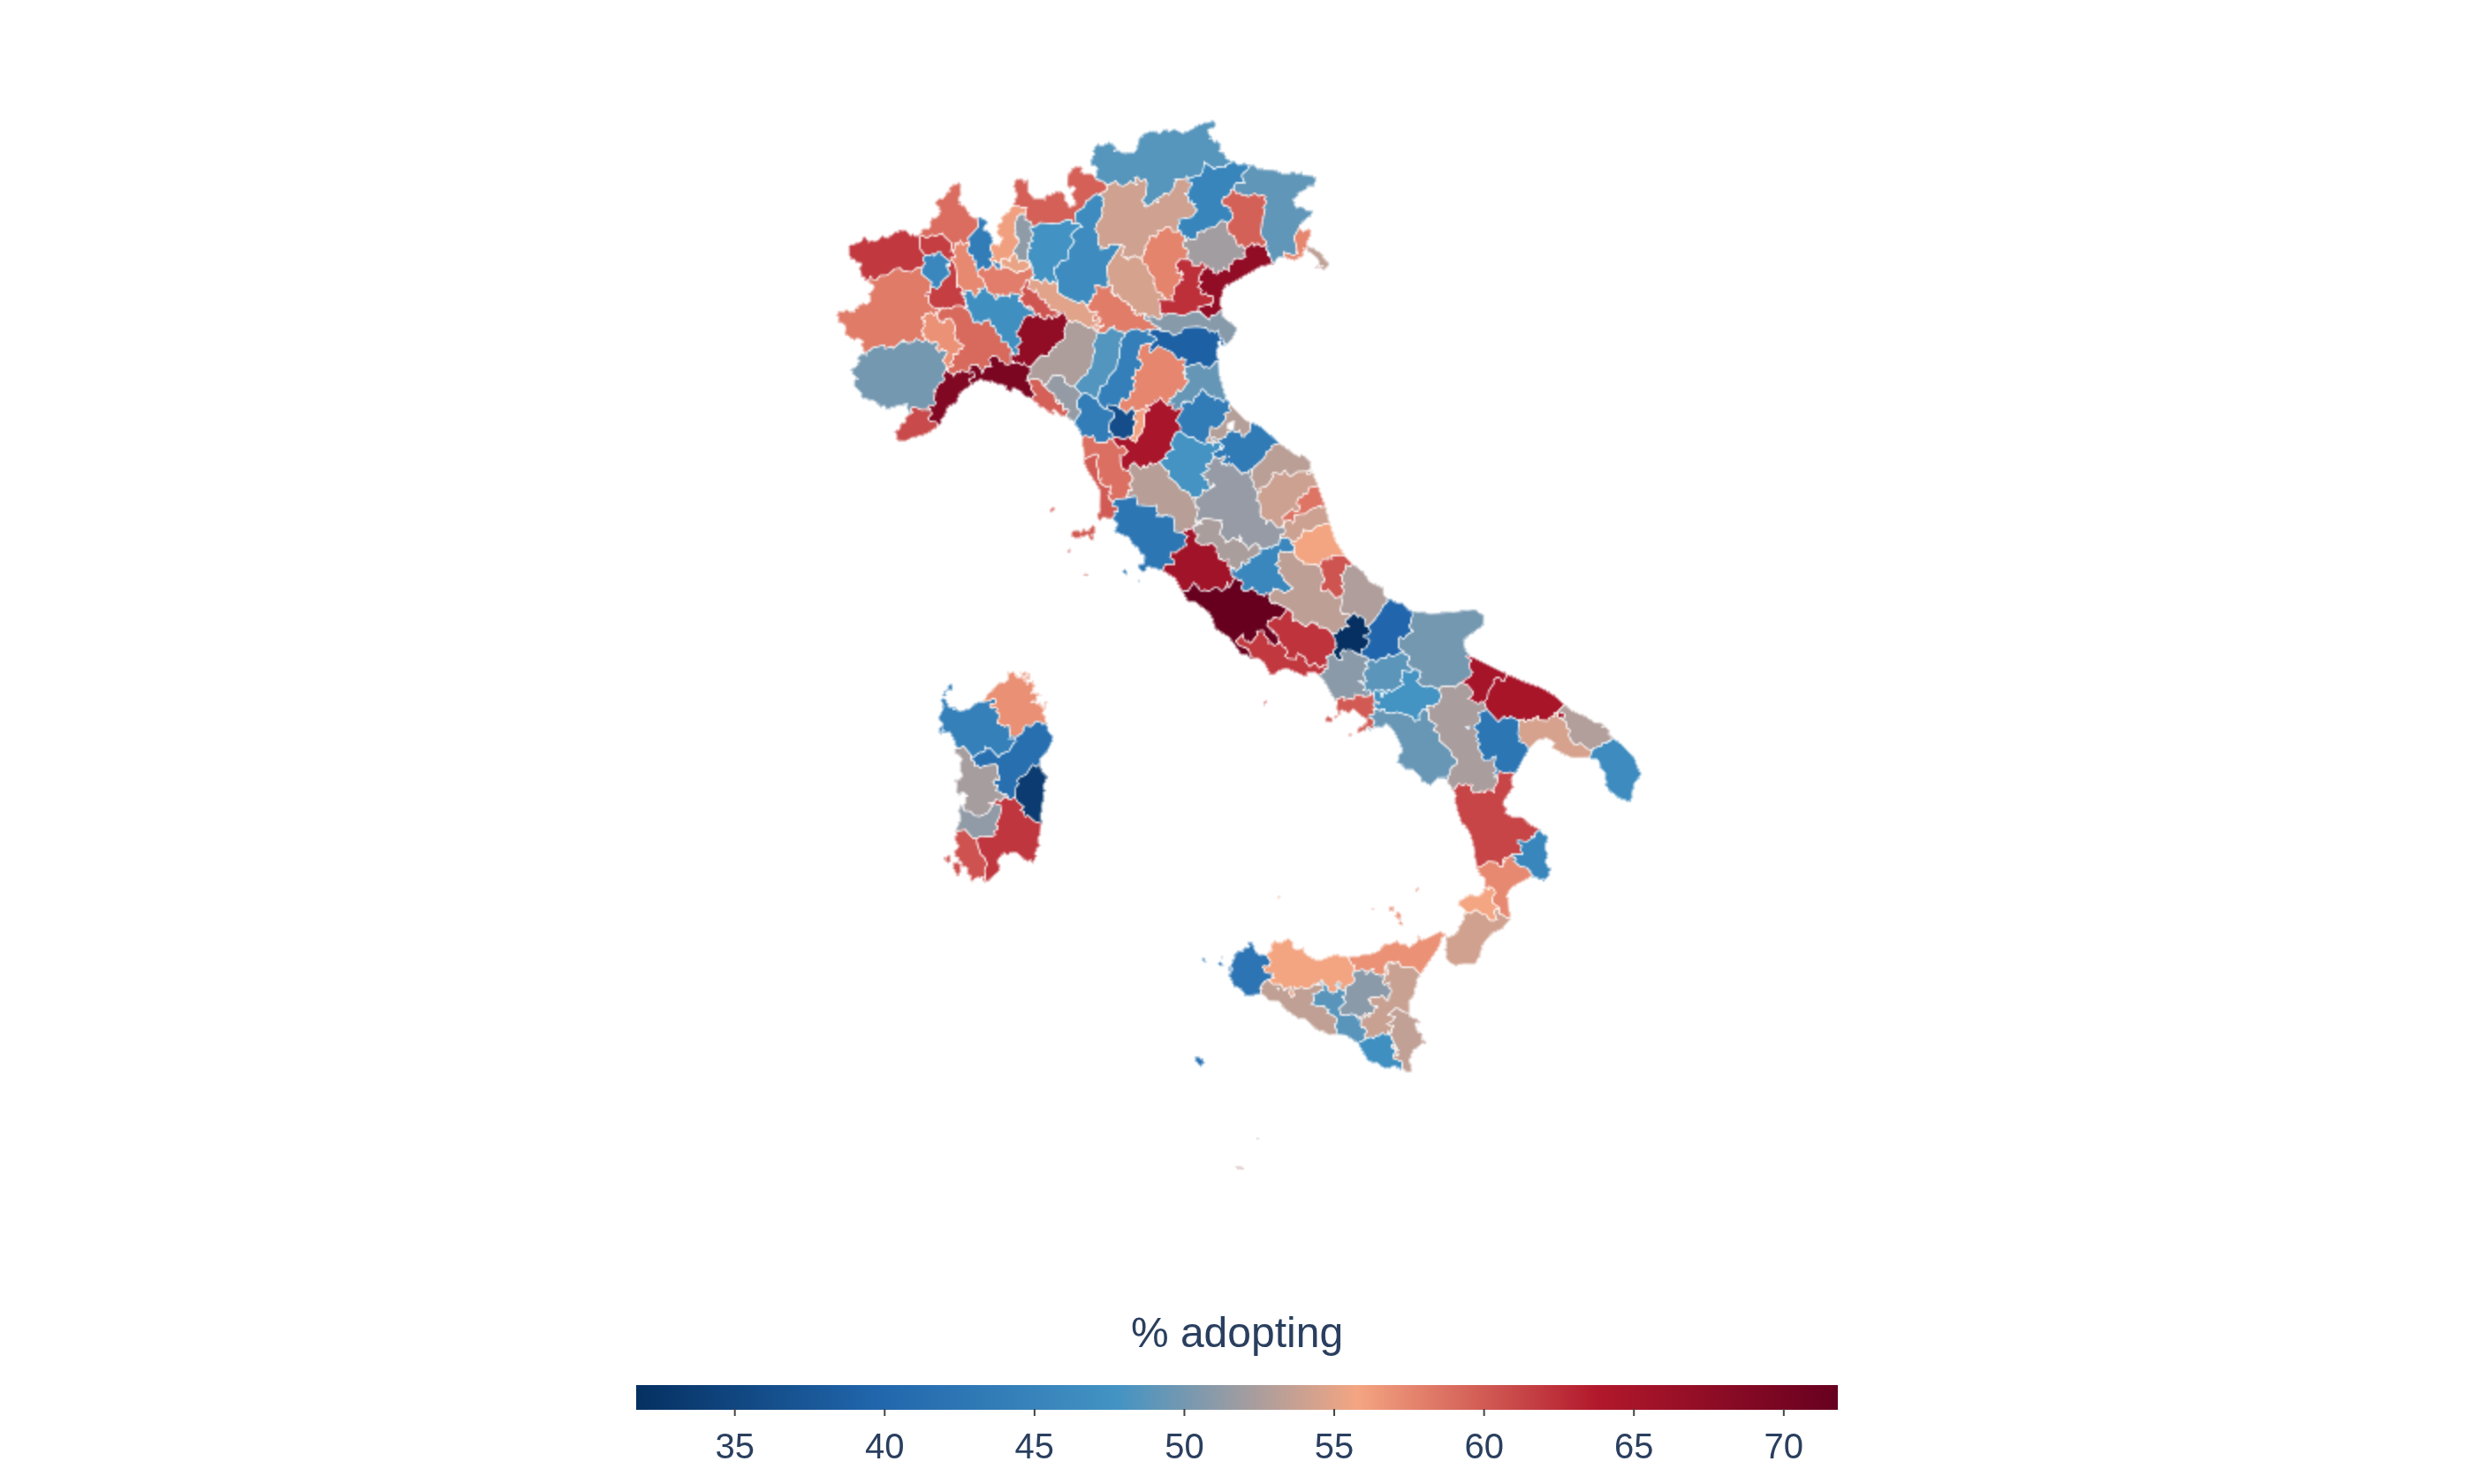
\includegraphics[width=0.8\textwidth]{output/figures/amap_adopt7_ben.png}
\caption{Petrol: share of units at or below the cap, 28 September --
5 October 2026 (\%).}
\label{fig:amadoptben}
\end{figure}

\begin{figure}[H]
\centering
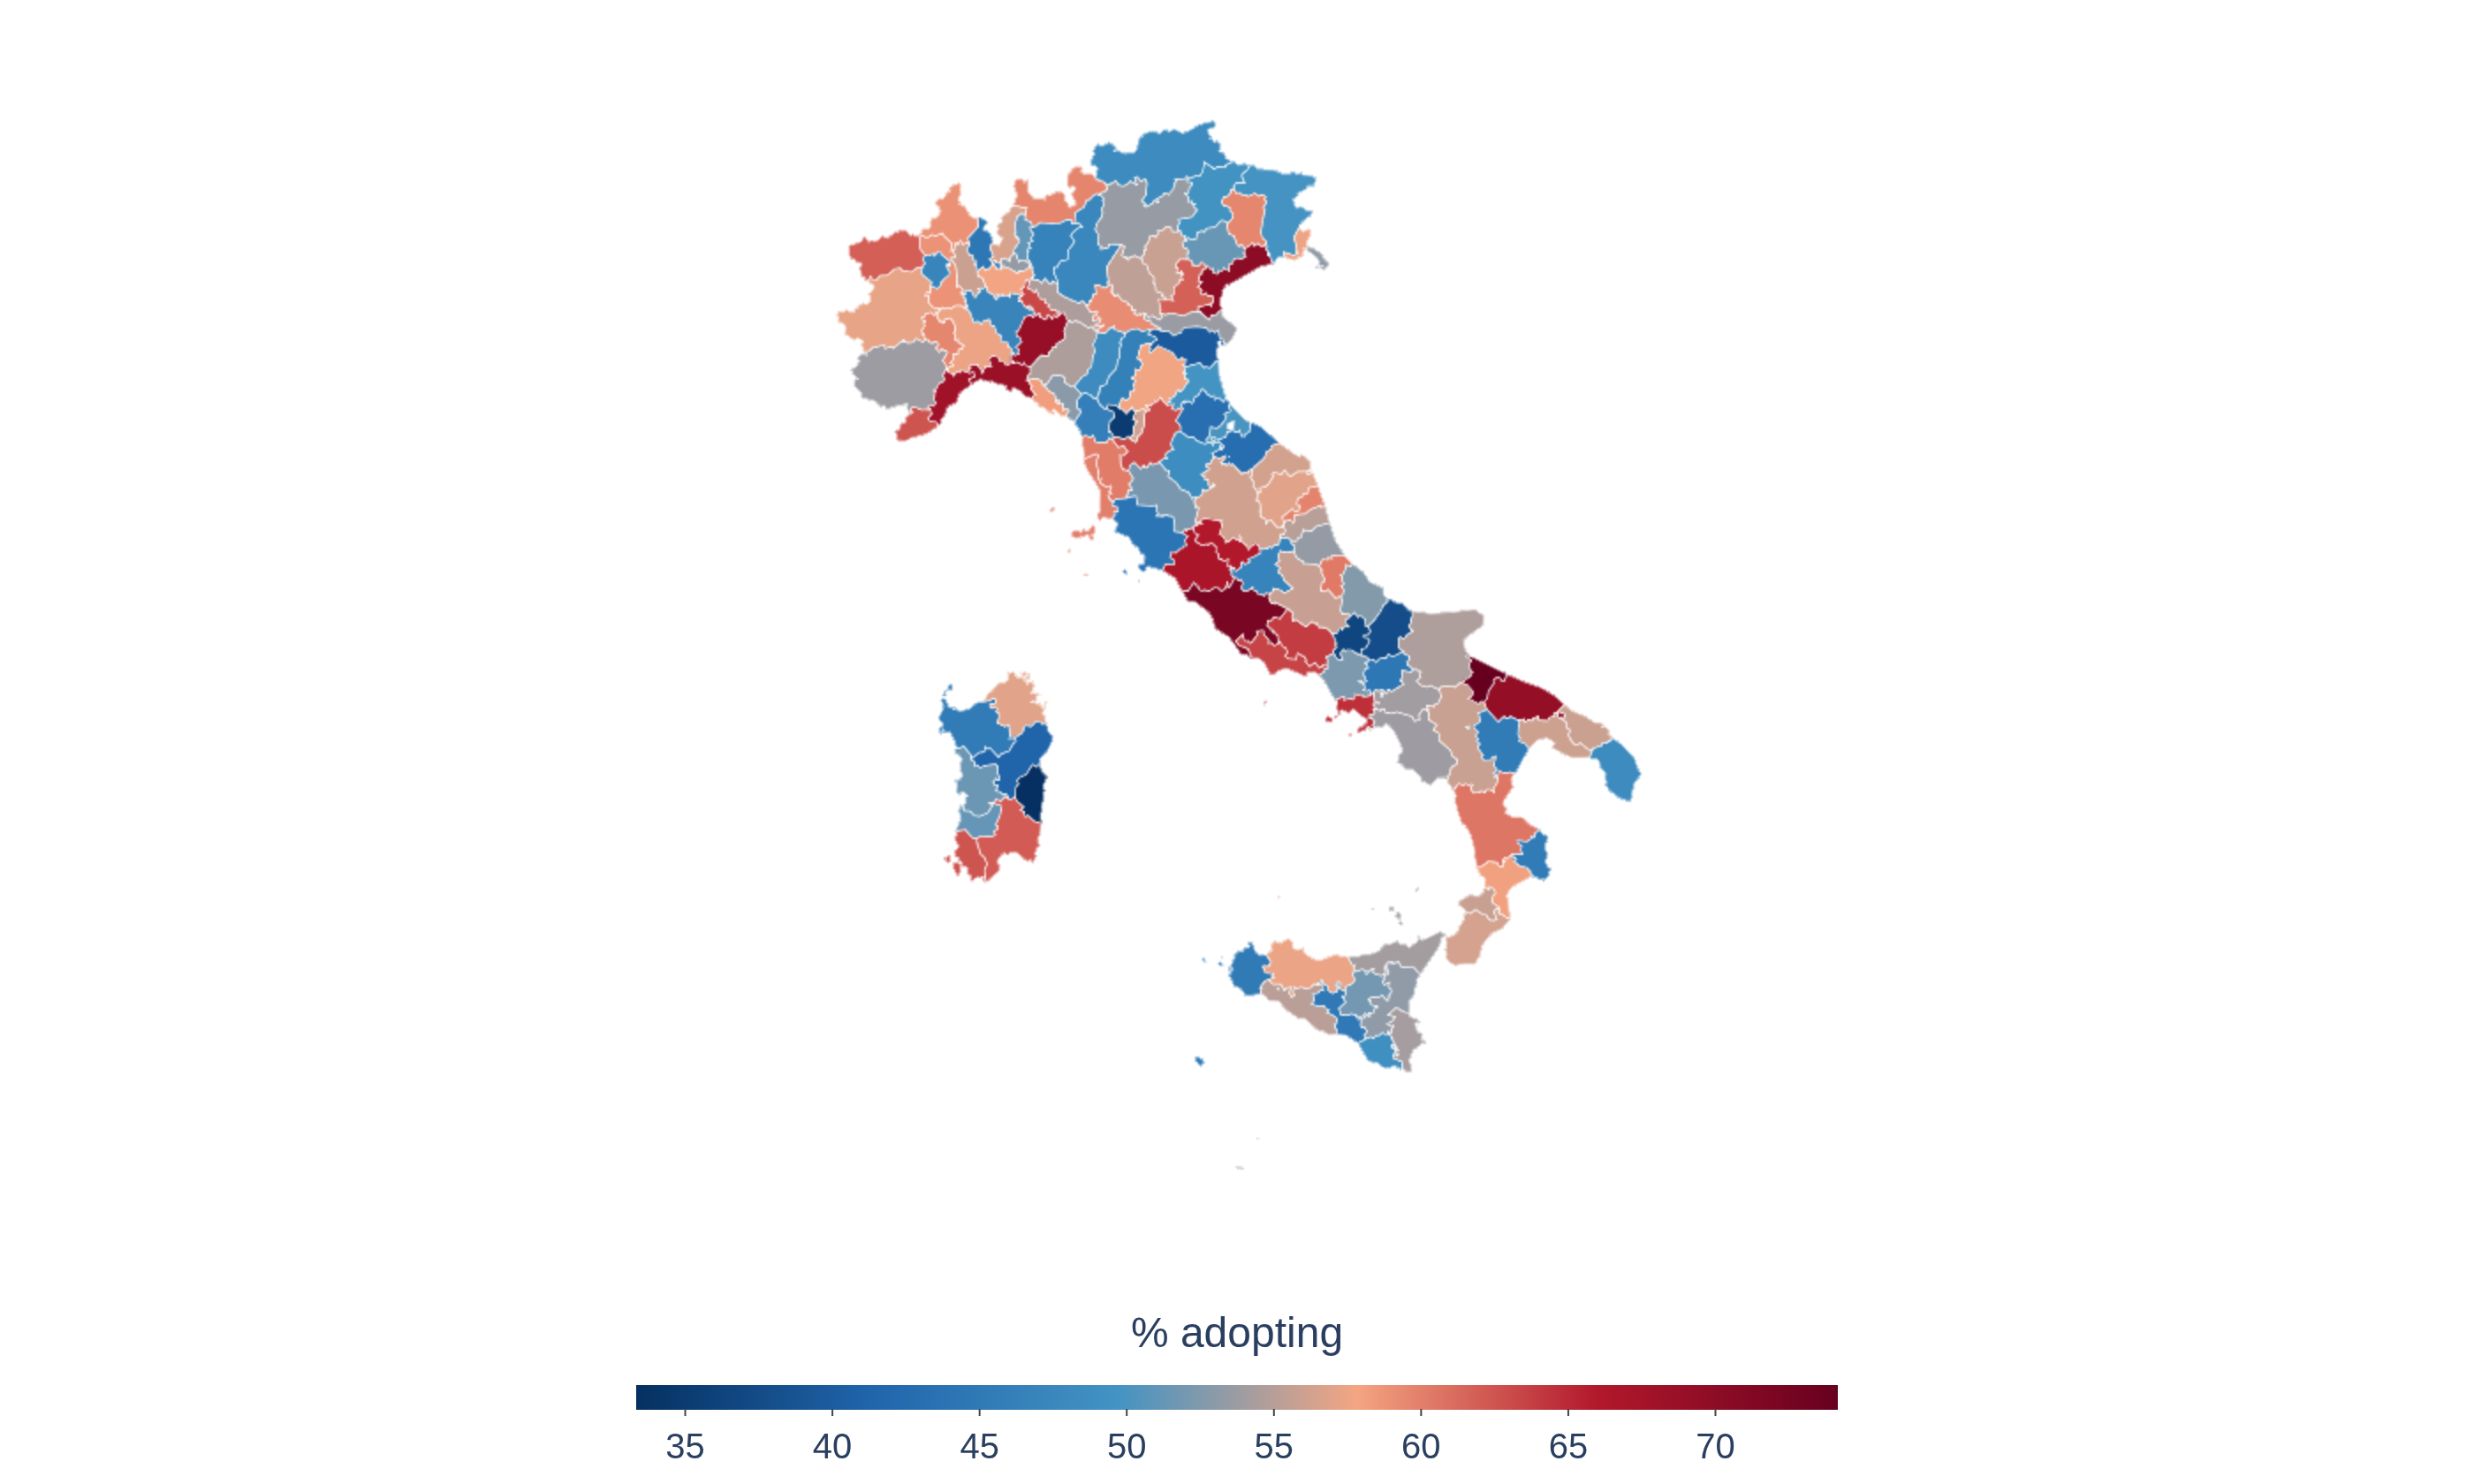
\includegraphics[width=0.8\textwidth]{output/figures/amap_adopt7_gas.png}
\caption{Diesel: share of units at or below the cap, 28 September --
5 October 2026 (\%).}
\label{fig:amadoptgas}
\end{figure}

\clearpage
\paragraph{Dispersion and the non-adopter gap across provinces
(main-text section \ref{sec:dispersion}).} The four maps behind the
distributions of \cref{fig:sdcapdist}: within-province price SD before
and after the cap, and the non-adopter gap before and after.

\begin{figure}[H]
\centering
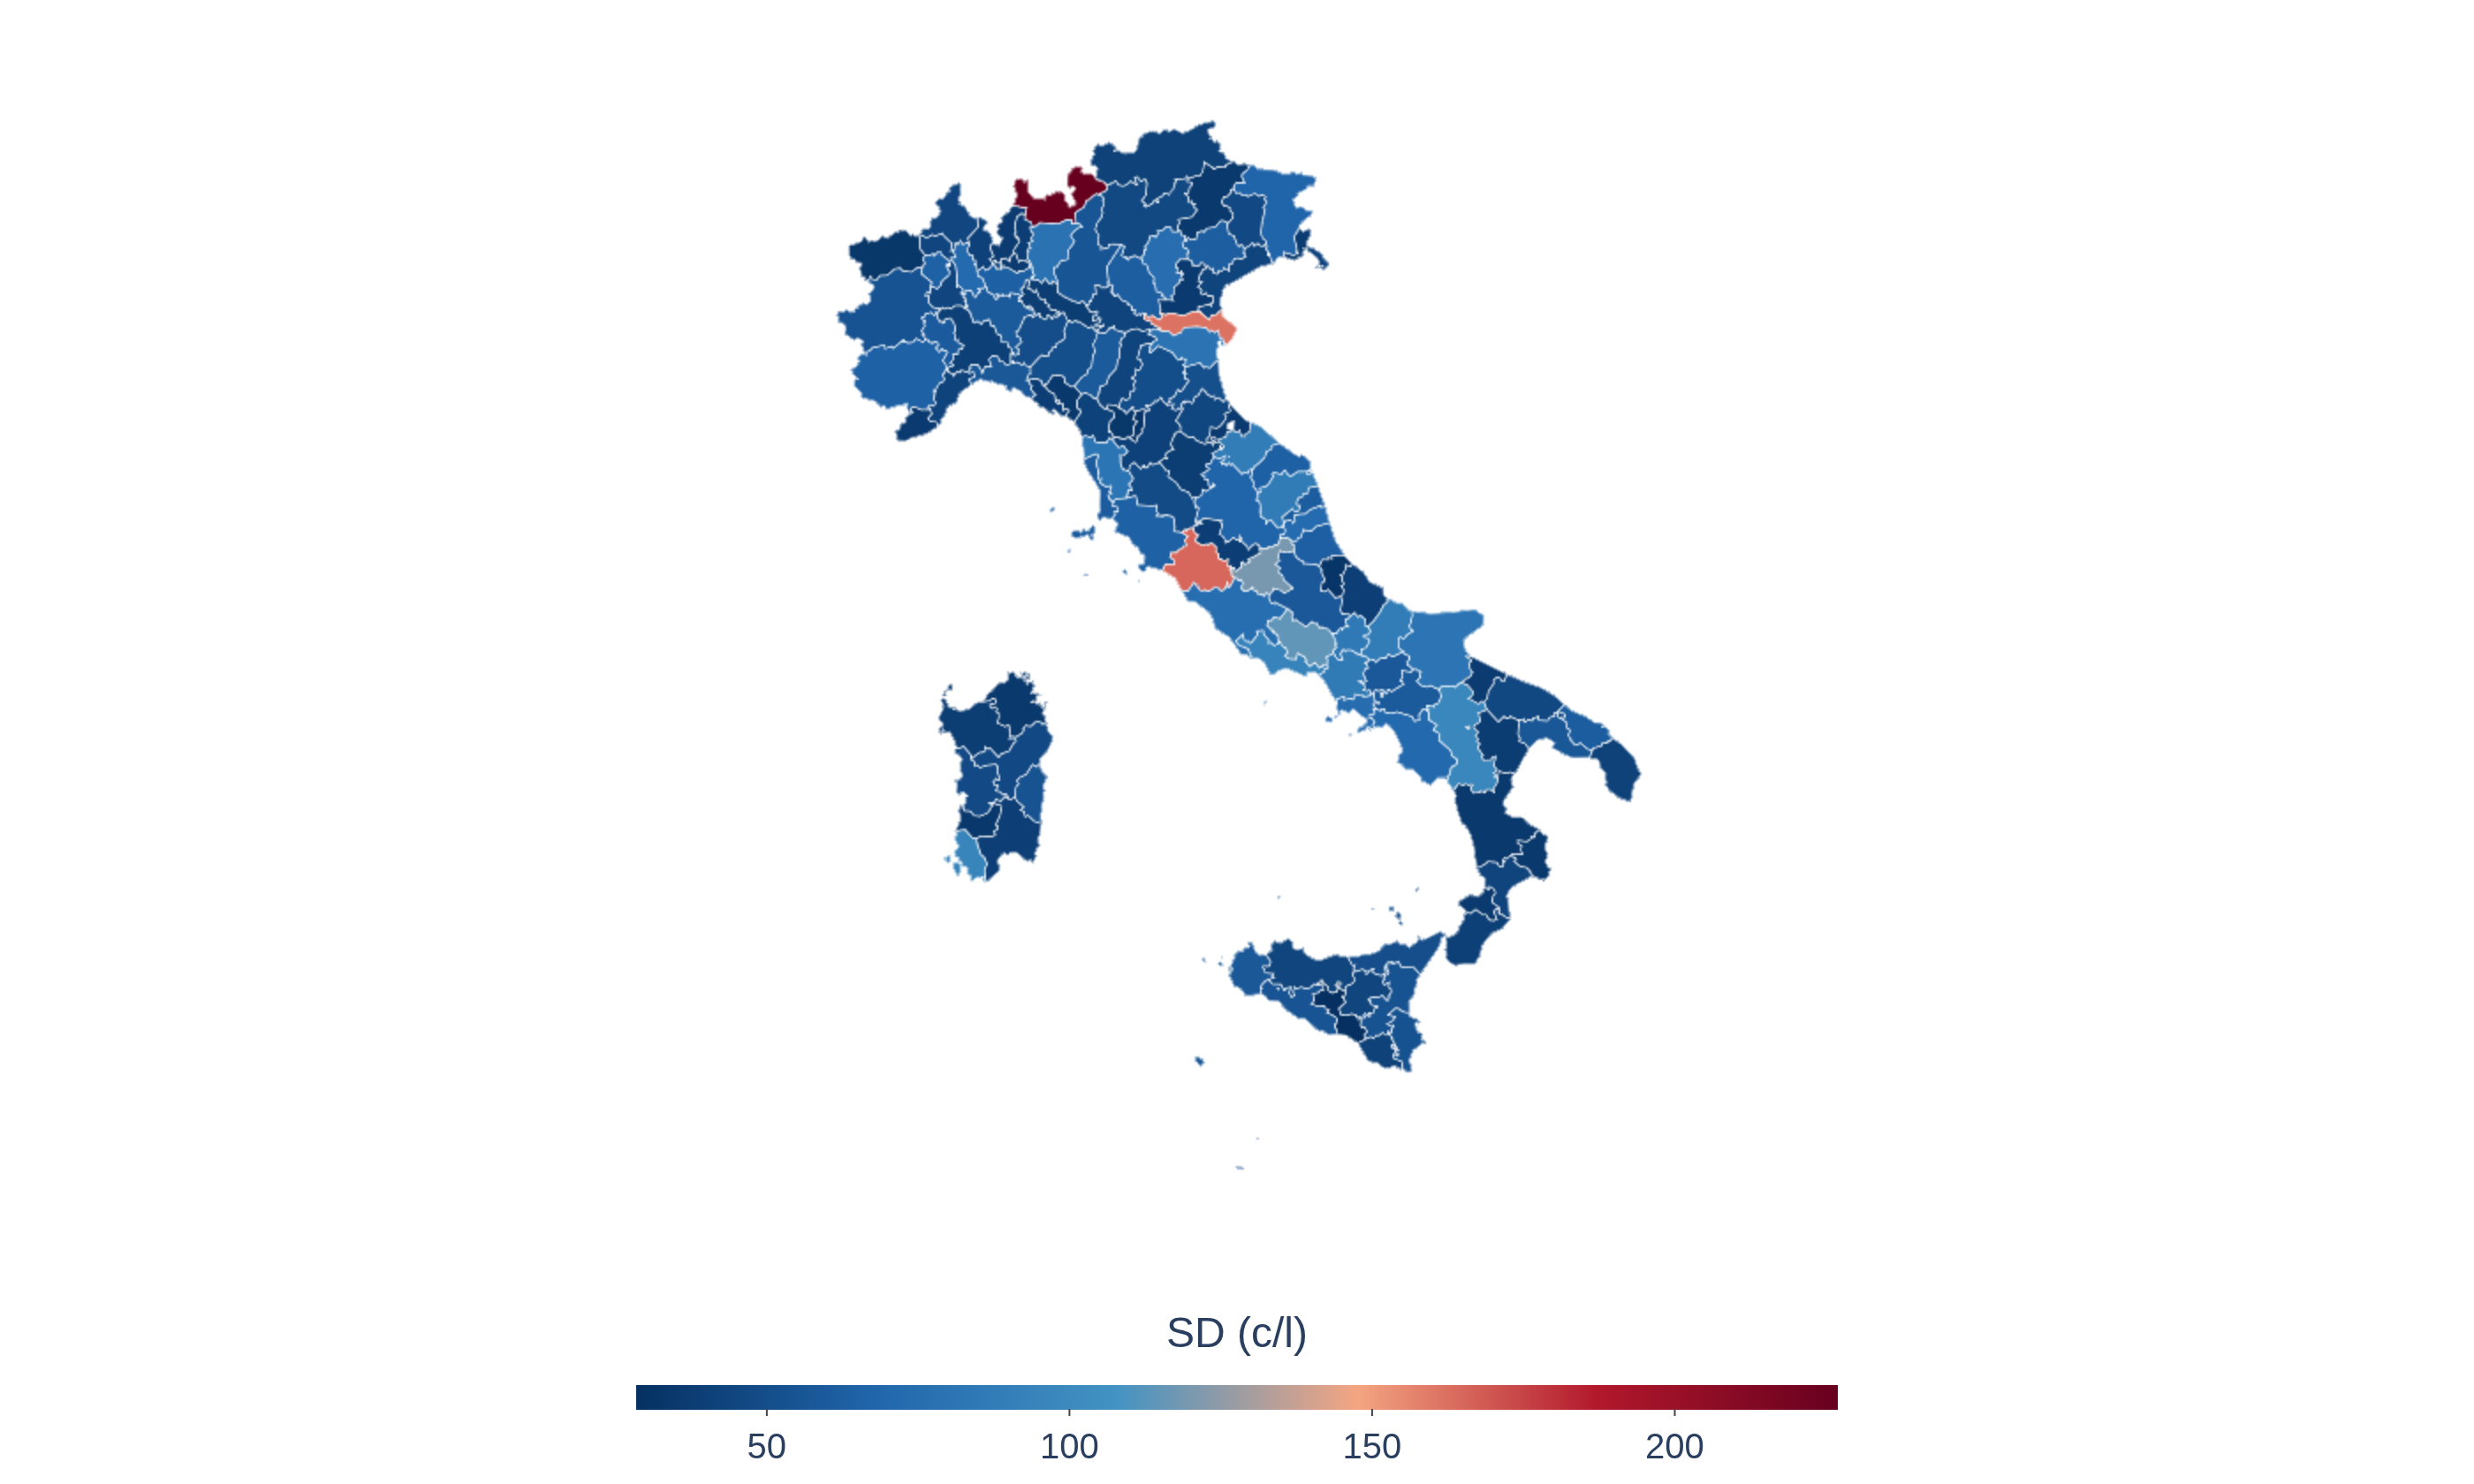
\includegraphics[width=0.8\textwidth]{output/figures/map_sd_pre.png}
\caption{Within-province standard deviation of effective prices (c/l),
pre-cap (21--27 September); mean across the two fuels. Red = high.}
\label{fig:sdpre}
\end{figure}

\begin{figure}[H]
\centering
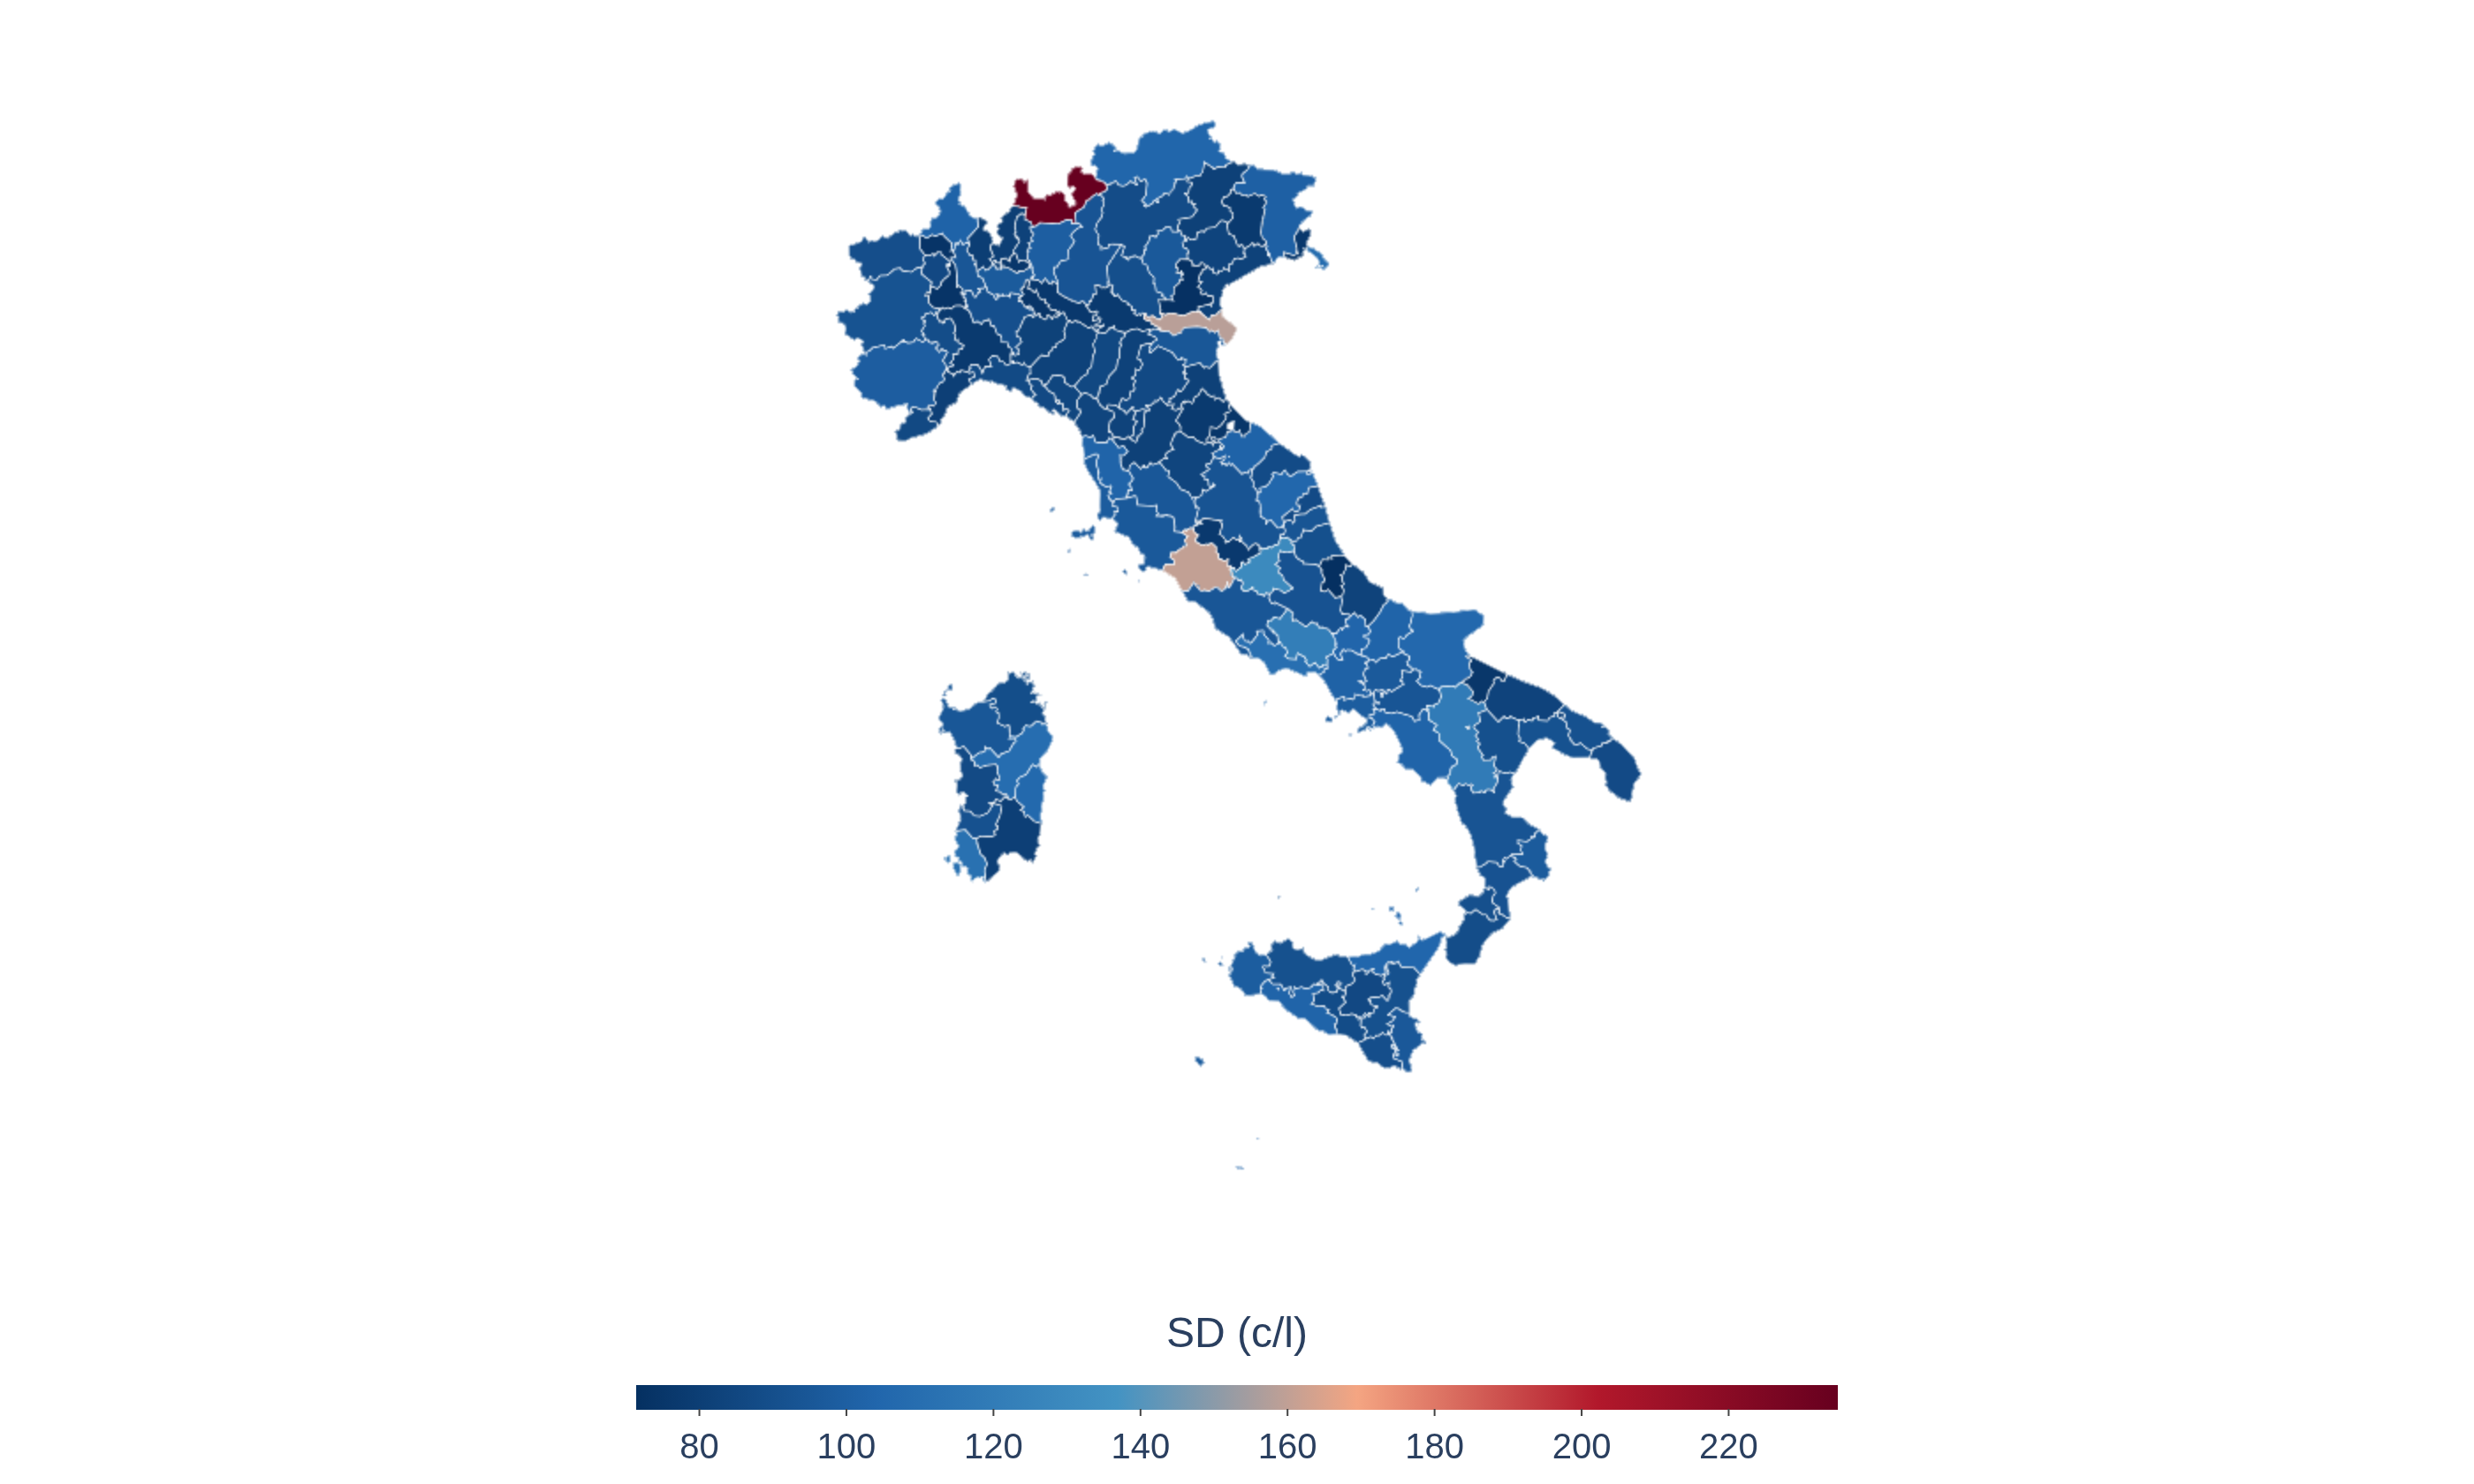
\includegraphics[width=0.8\textwidth]{output/figures/map_sd_post.png}
\caption{Within-province standard deviation of effective prices (c/l),
post-cap (28 September -- 7 October); mean across the two fuels.
Red = high.}
\label{fig:sdpost}
\end{figure}

\begin{figure}[H]
\centering
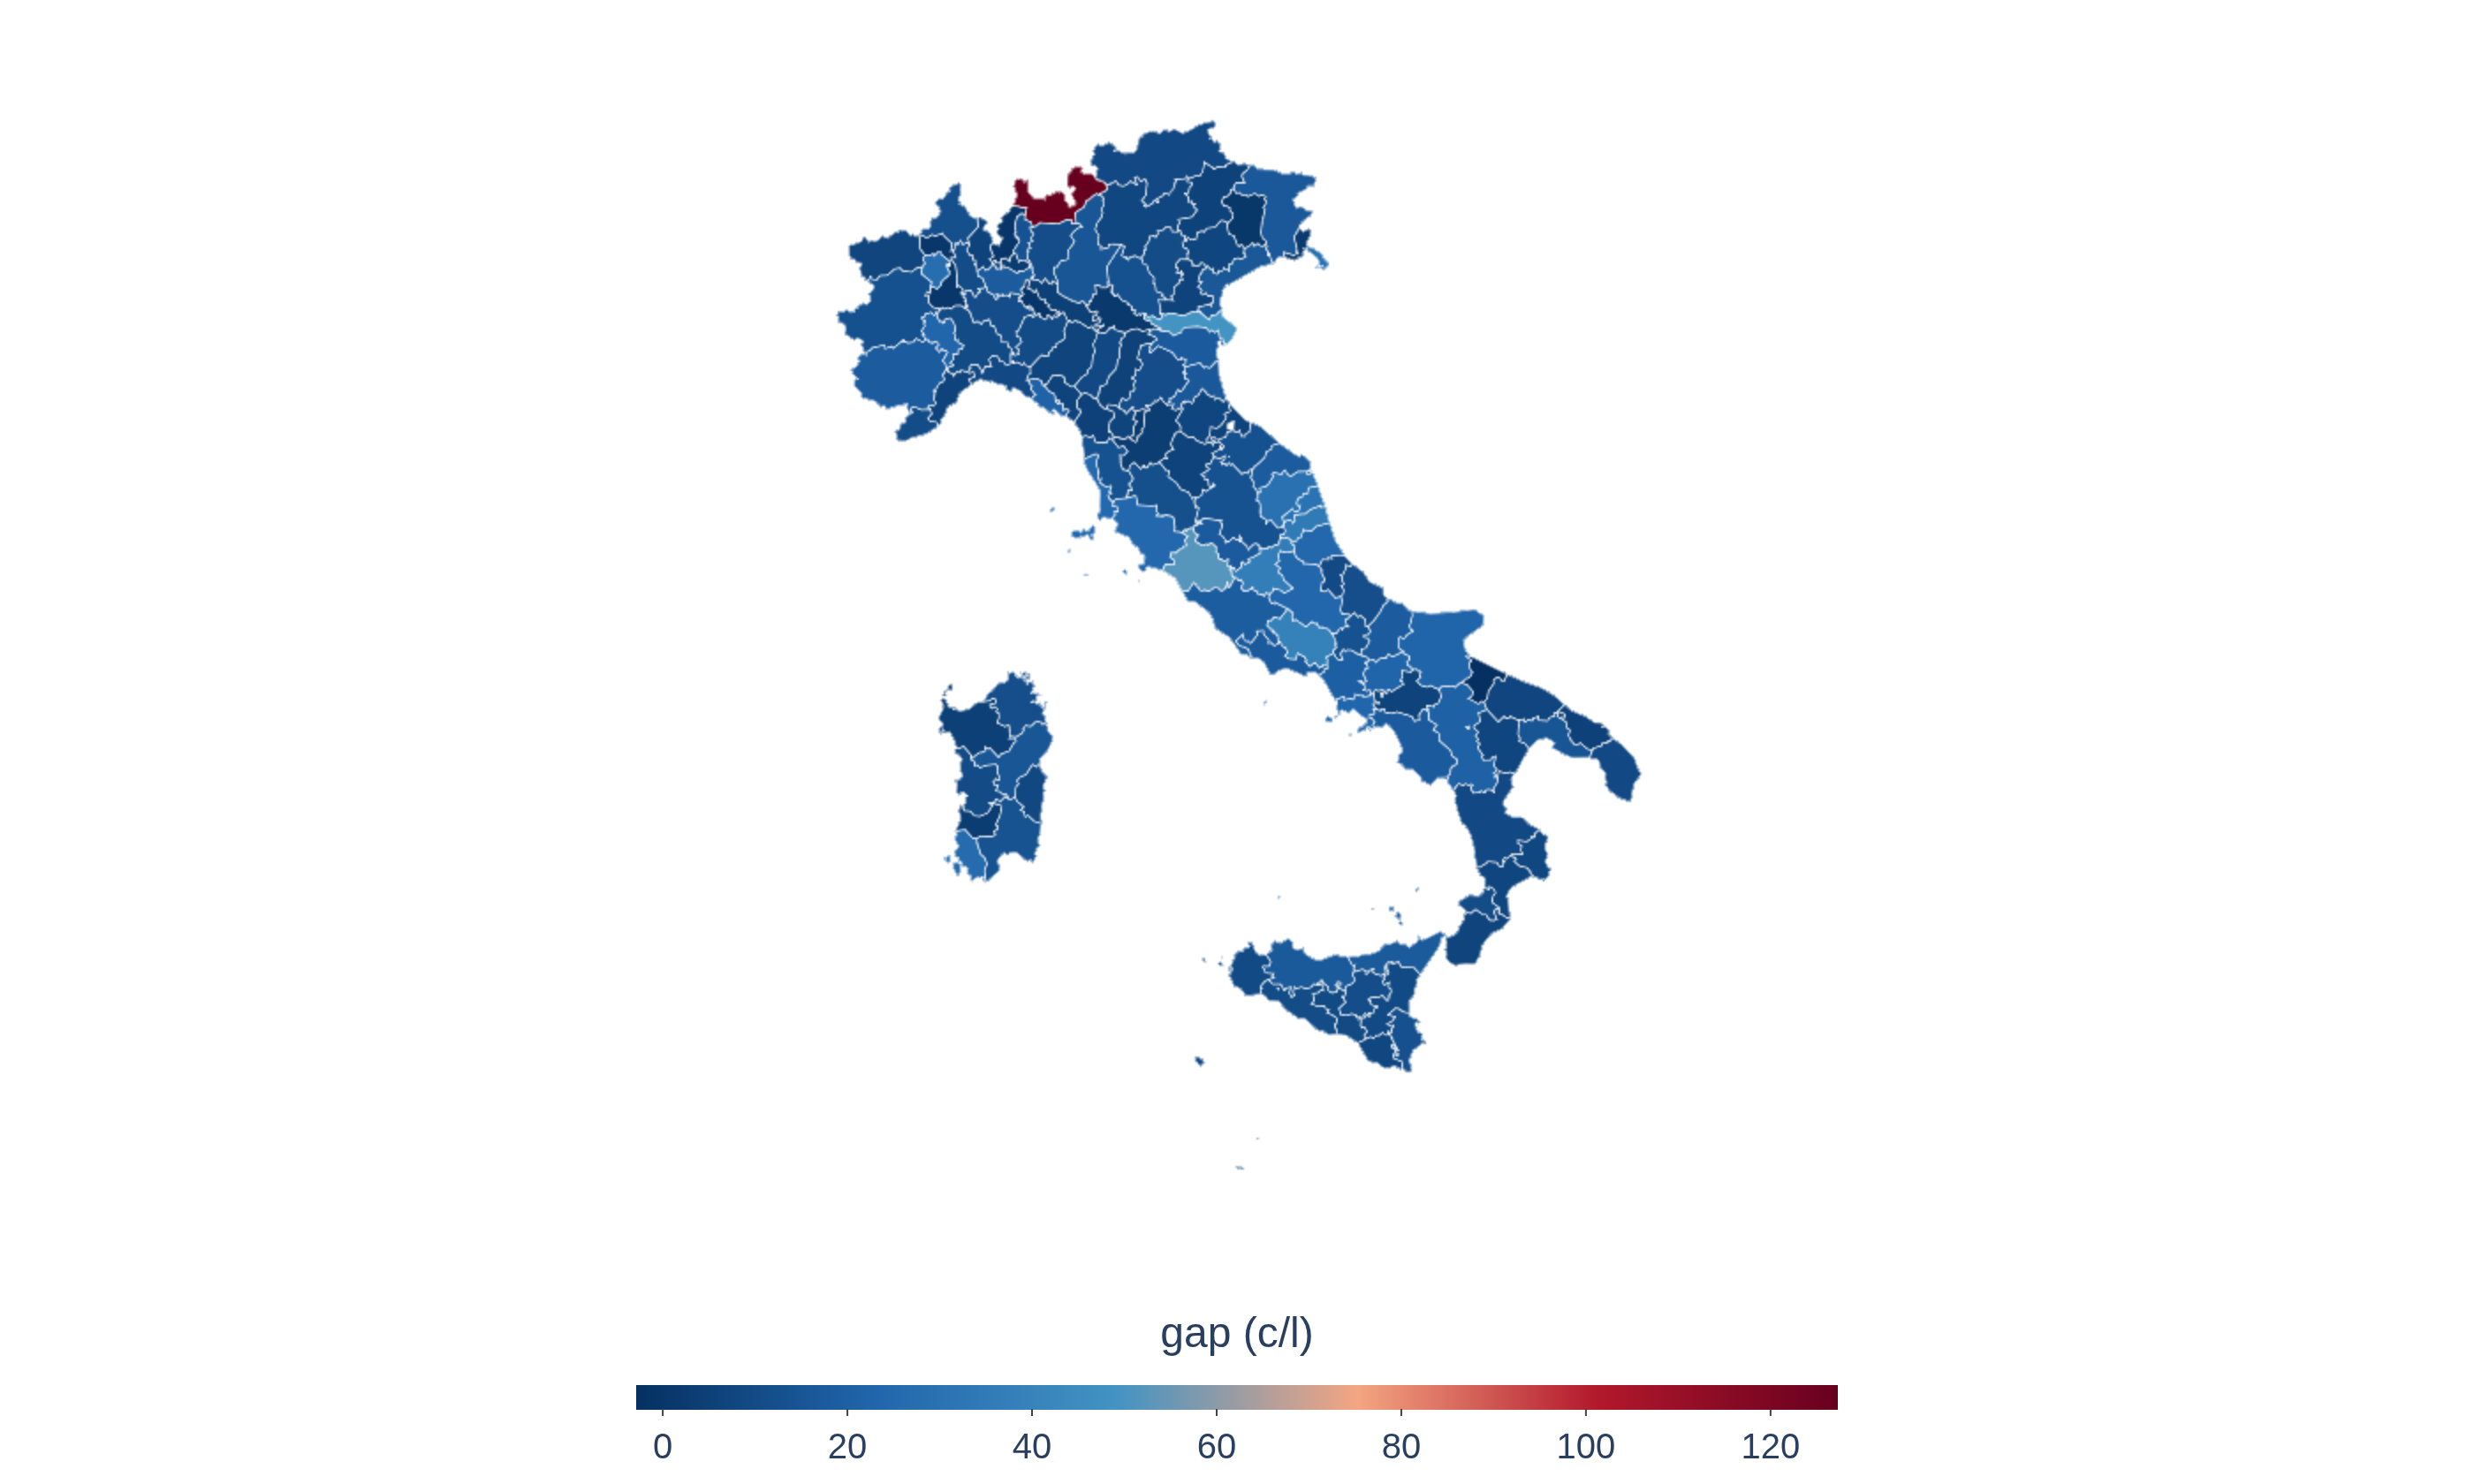
\includegraphics[width=0.8\textwidth]{output/figures/map_gap_pre.png}
\caption{Non-adopters' mean gap to the provincial daily mean (c/l),
pre-cap. Red = large gap.}
\label{fig:gappre}
\end{figure}

\begin{figure}[H]
\centering
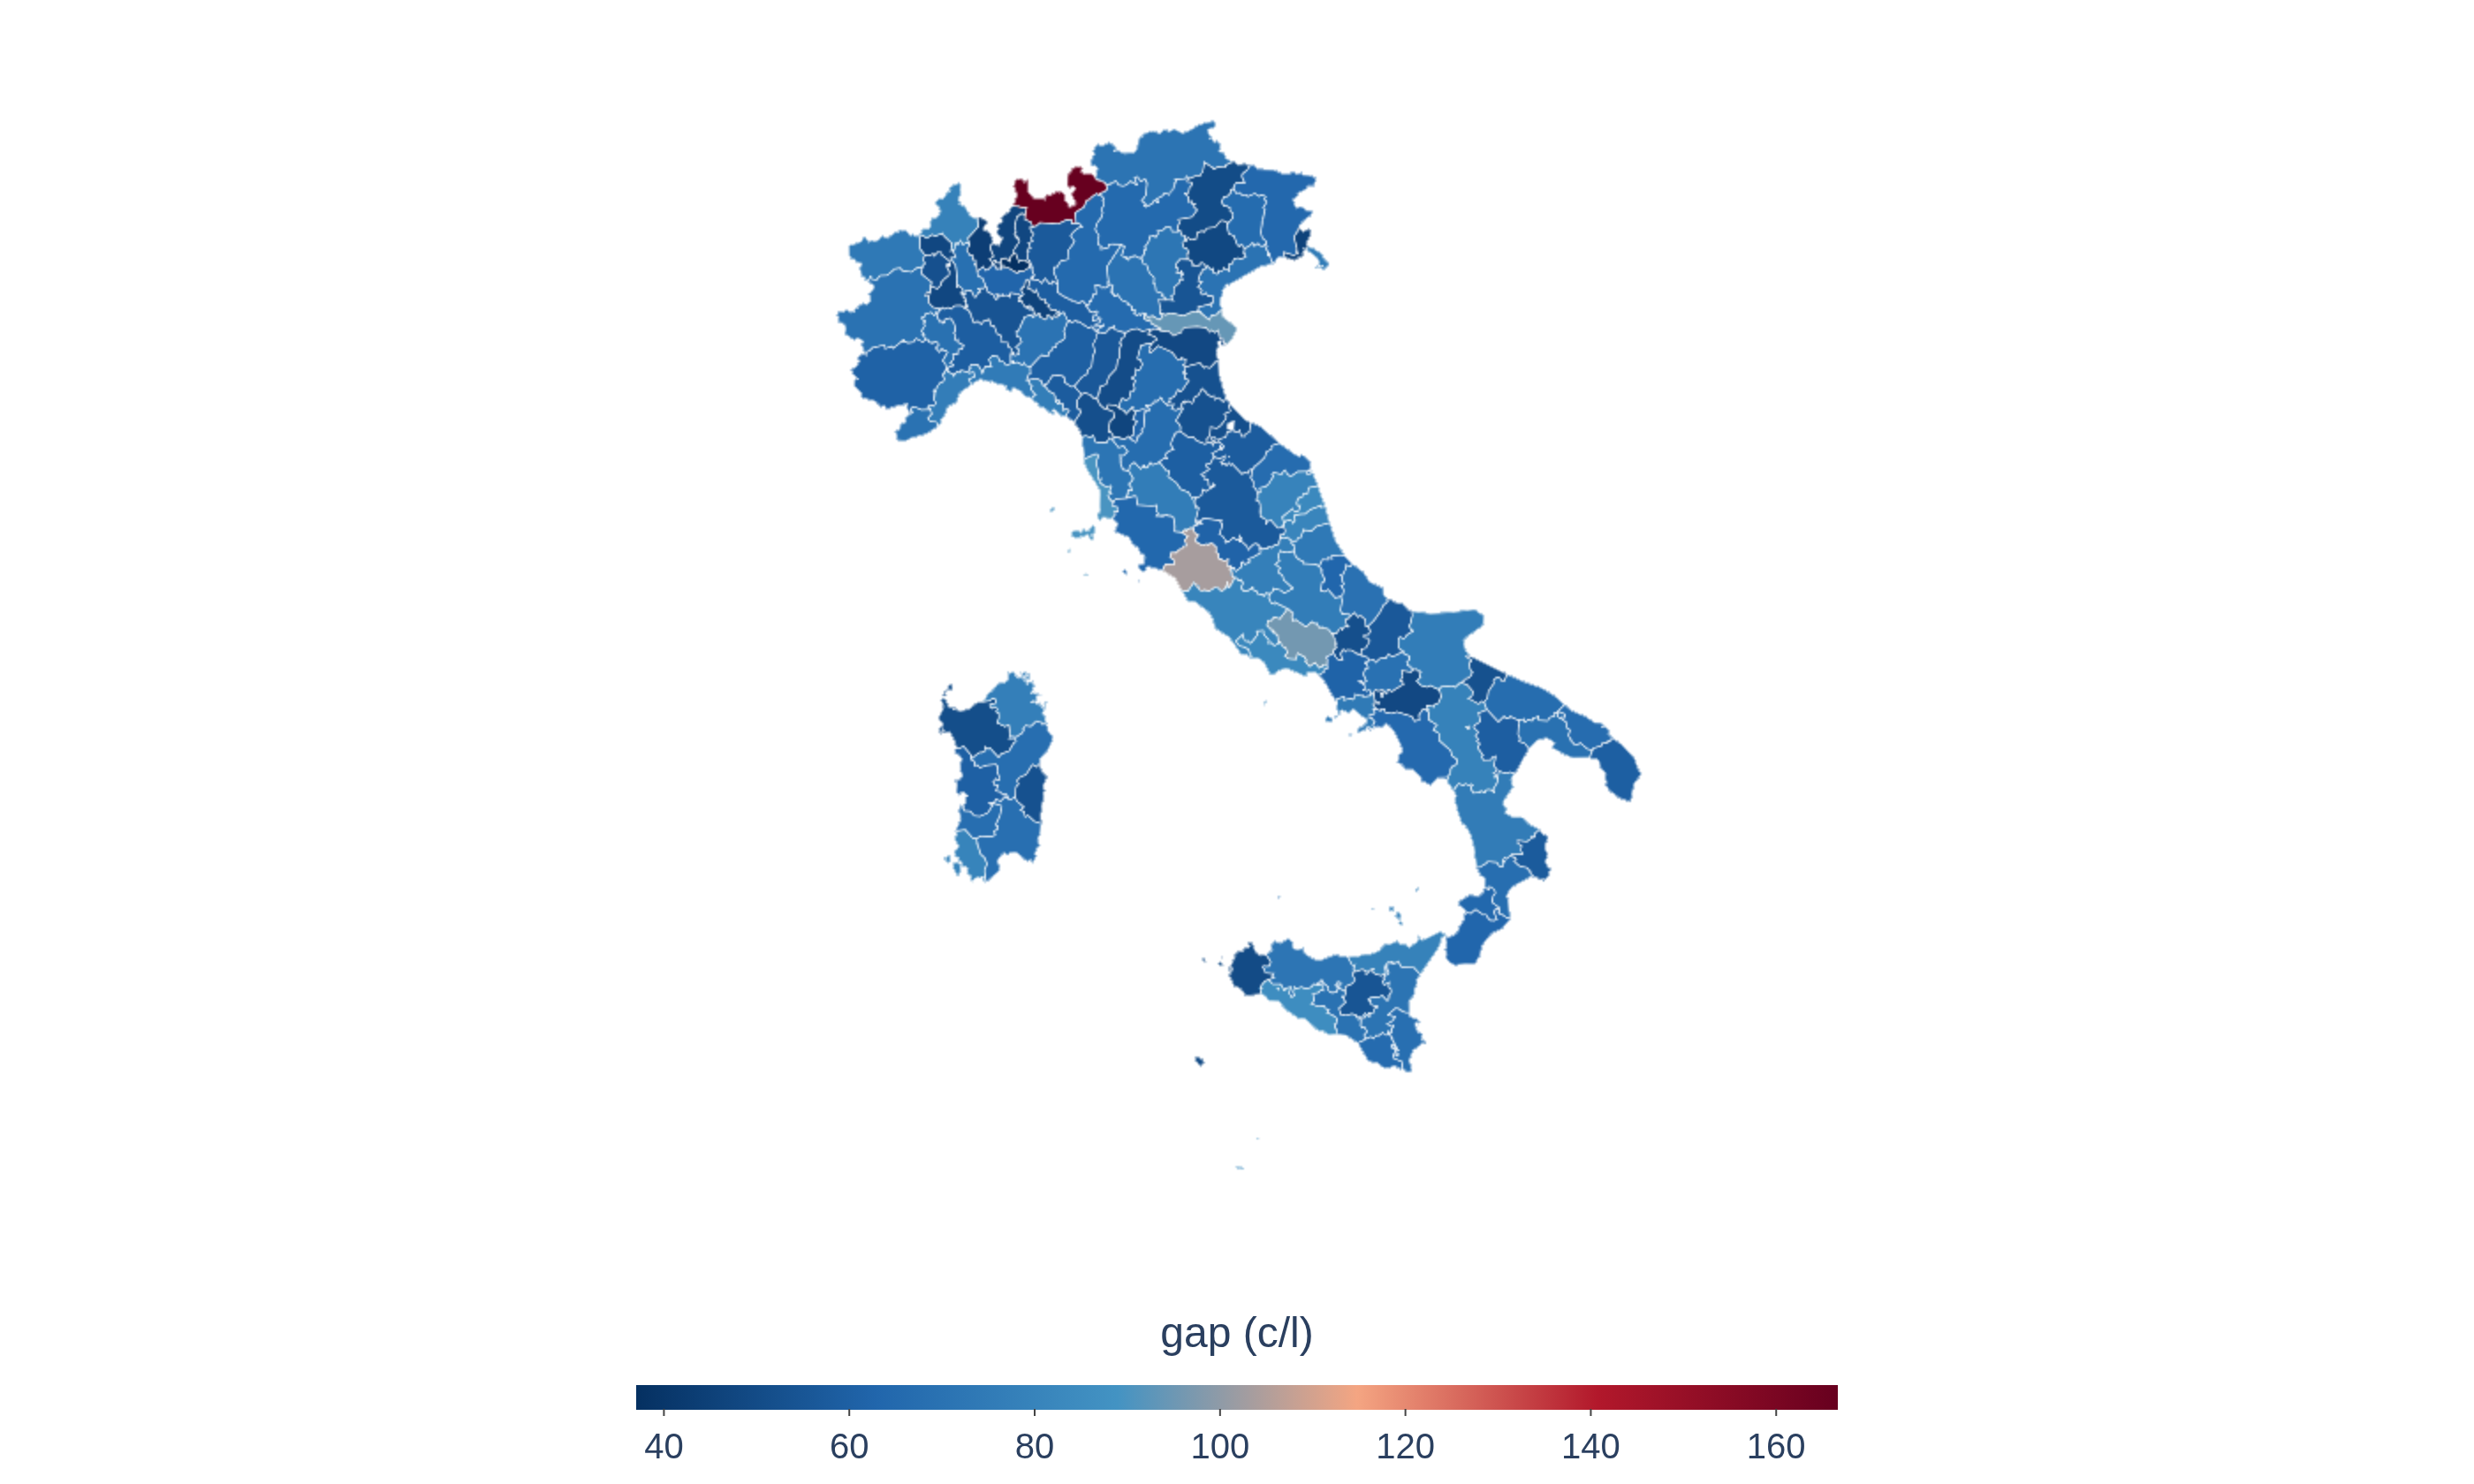
\includegraphics[width=0.8\textwidth]{output/figures/map_gap_post.png}
\caption{Non-adopters' mean gap to the provincial daily mean (c/l),
post-cap (28 September -- 7 October). Red = large gap.}
\label{fig:gappost}
\end{figure}

\end{document}
